%*******10********20********30********40********50********60********70********80
%% ----------------------------------------------------------------
%% Thesis.tex -- MAIN FILE (the one that you compile with LaTeX)
%% ---------------------------------------------------------------- 
%% This template is based on Graduate Thesis written by Sunil Patel,

% (ho based it on the ecsthesis template) under the LaTeX Project Public License.
% which can be found here: http://latex-project.org/lppl/
% in the hope that it will be easier to use and to scale down to your needs
% by Simon Ternsjö in 2013-10
% INSTRUCTIONS:
% The meaning is not to edit this document much, but to fill in information 
% in the different files in the folders;
% Settings, Frontpages, Chapters, Appendices and possibly Files,
% as well as the file Bibliography.bib
% This template is easy to scale down to suite your need, 
% simply comment the input statements explained below
% Set up the document:
\documentclass[a4paper, 11pt, oneside]{Thesis}  % Use the "Thesis" style, based on the ECS Thesis style by Steve Gunn

% Add more package in Package.tex:
% Add your own packages here, 
% these existing packages can be removed if necessary
% not that more packages are imported in Thesis.cls, '
%  but those should not be changed if you don't know what you are doing...


\usepackage[utf8]{inputenc} % for writing other that basic characters
\usepackage{graphicx}
\usepackage{caption}
\usepackage{subcaption}
\usepackage{multicol}
\usepackage[dvipsnames*,svgnames]{xcolor}
\usepackage{listings}
\usepackage{hyperref}
\usepackage{float}
\usepackage{multirow}
\usepackage{bookmark}


% Include any extra LaTeX packages required
\usepackage[square, numbers, comma, sort&compress]{natbib}  % Use the "Natbib" style for the references in the Bibliography
\usepackage{verbatim}  % Needed for the "comment" environment to make LaTeX comments
%5%\usepackage{vector}  % Allows "\bvec{}" and "\buvec{}" for "blackboard" style bold vectors in maths

\DeclareFixedFont{\ttb}{T1}{txtt}{bx}{n}{12} % for bold
\DeclareFixedFont{\ttm}{T1}{txtt}{m}{n}{12}  % for normal
\definecolor{deepblue}{rgb}{0,0,0.5}
\definecolor{deepred}{rgb}{0.6,0,0}
\definecolor{deepgreen}{rgb}{0,0.5,0}

% Python style for highlighting
\lstset{
	backgroundcolor = \color{Ivory},
    language=Python,
    basicstyle=\footnotesize,
    otherkeywords={self},             
    keywordstyle=\footnotesize\color{deepblue},
    emph={__init__},          
    emphstyle=\footnotesize\color{deepred},    
    stringstyle=\color{deepgreen},
    frame=single,                         
    showstringspaces=false  ,
    breaklines=true,
    numbers=left,
    numberstyle=\footnotesize,
    tabsize=3,
    breakatwhitespace=false
}

\hypersetup{
    linkcolor=black,
    filecolor=magenta,      
    urlcolor=blue,
}

% Use if you want:
%5%\graphicspath{Figures/}  % Location of the graphics files (set up for graphics to be in PDF format)
%5%\hypersetup{urlcolor=blue, colorlinks=true}  % Colours hyperlinks in blue, but this can be distracting if there are many links.

% Set your name, the title of the report and more in Administraitve.tex:
% This is where author, university, title and more is defined

% Personal information:
\newcommand{\myAuthorName}  {Andrea Spreafico}% Author Name
\newcommand{\myAuthorEmail} {asp005@post.uit.no} % Author email
\newcommand{\myTitle}       {Data Science using Python: \\ Analysis of Salmon farming in Norway} % Thesis title goes here
\newcommand{\mySubject}     {Computer Science} % Subject goes here
\newcommand{\myKeywords}    {Aquaculture, Fishery} % Keywords goes hear

% An initial approach to Data Science using Python: Analysis about Norwegian salmon farming.

% Data Science with Python for salmon farming analysis in Norway

% Data Science with Python for salmon farming prediction in Norway

% Data Science using Python: Initial analysis of salmon farming in Norway


% University information
\newcommand{\myUniversity}{University of Tromsø} %The Iniversity name goes here
\newcommand{\myUniversityWeb}{https://en.uit.no/startsida} %University Web Site URL Here (include http://
\newcommand{\myDepartment}{Department of Computer Science} % The Department goes here 
\newcommand{\myDepartmentWeb}{https://en.uit.no/om/enhet/forsiden?p_dimension_id=88138} % Department Web Site URL Here (include http://)
\newcommand{\myFaculty}{Faculty of Computer Science}
\newcommand{\myFacultyWeb}{https://uit.no/utdanning/program?p_document_id=279505}

%Degree, program or corse: ex: Master of Science, Engineering Physics
\newcommand{\myDegree}{Computer Science} % The degree, program or course-name goes here


% can be left untouched, both:
\newcommand{\myDate}{\today}
\newcommand{\myPartyalFulfillment}{A thesis submitted in partial fulfillment for the degree of Computer Science}


%% ----------------------------------------------------------------
\begin{document}

\frontmatter      % Begin Roman style (i, ii, iii, iv...) page numbering


% Here the first pages are imported, you can find them in the Frontpages folder
% Files in the subfolder Fixed does not need to be edited.
% If you don't need any of these sections, simply comment, or delete, the input-row\dfrac{•}{•}


%% All the pages before the chapters ------------------------------
% Set up the Title Page - DO NOT EDIT THIS, (if you don't want to ;)  )
% instead specify your name, title and more in "/Settings/Administrative.tex"
\title   {\myTitle}
\authors {\texorpdfstring
            {\href{\myAuthorEmail}{\myAuthorName}}
            {\myAuthorName}
         }
\addresses  {\groupname\\\deptname\\\univname}  
\date       {\myDate}
\subject    {\mySubject}
\keywords   {\myKeywords}

\maketitle
%% ----------------------------------------------------------------

\setstretch{1.3}  % It is better to have smaller font and larger line spacing than the other way round

% Define the page headers using the FancyHdr package and set up for one-sided printing
\fancyhead{}  % Clears all page headers and footers
\rhead{\thepage}  % Sets the right side header to show the page number
\lhead{}  % Clears the left side page header


% %% ----------------------------------------------------------------
% Declaration Page required for the Thesis, your institution may give you a different text to place here
\pagestyle{fancy}  % Finally, implement the FancyHdr headers
\clearpage
\Declaration{

\addtocontents{toc}{\vspace{1em}}  % Add a gap in the Contents, for aesthetics

I, \myAuthorName, declare that this thesis titled, `\myTitle' and the work presented in it are my own. I confirm that:

\begin{itemize} 
\item[\tiny{$\blacksquare$}] This work was done wholly or mainly while in candidature for a research degree at this University.
 
\item[\tiny{$\blacksquare$}] Where any part of this thesis has previously been submitted for a degree or any other qualification at this University or any other institution, this has been clearly stated.
 
\item[\tiny{$\blacksquare$}] Where I have consulted the published work of others, this is always clearly attributed.
 
\item[\tiny{$\blacksquare$}] Where I have quoted from the work of others, the source is always given. With the exception of such quotations, this thesis is entirely my own work.
 
\item[\tiny{$\blacksquare$}] I have acknowledged all main sources of help.
 
\item[\tiny{$\blacksquare$}] Where the thesis is based on work done by myself jointly with others, I have made clear exactly what was done by others and what I have contributed myself.

\end{itemize}
 
\vspace{10 mm}
 
Signed:\\
\rule[1em]{25em}{0.5pt}  % This prints a line for the signature

Date:\\
\rule[1em]{25em}{0.5pt}  % This prints a line to write the date
}



% % The "Funny Quote Page"
\clearpage
\pagestyle{empty}  % No headers or footers for the following pages

%use 1 or vfill to position the quote where it looks good:
\null\vfill\vfill


% Now comes the "Funny Quote", written in italics:

\textit{
    % Write a funny quote here:
    ''We did it, we bashed them, wee Potter’s the one, \\
    and Voldy’s gone moldy, so now let’s have fun!''
}
\begin{flushright}
    % If the quote is taken from someone, their name goes here:
    - Peeves
\end{flushright}


 
\vfill\vfill\vfill\vfill\vfill\null


% The Abstract Page
\clearpage 

\chapter{Abstract}

The term Data Science refers to the collection of knowledges and skills, mainly about statistics and computer science, that allow to collect, analyze and display data in order to understand actual phenomena. To extract the needed informations from the data there isn't a default technique. This study investigates about the possibility of implementing an informations extraction system using Python. This kind of systems might be used for high interest area, such as the Aquaculture industry, that is a particular relevant industry in the norwegian economy, since Norway represents the forefront of innovation and development in this area.
 





% The Acknowledgements page, for thanking everyone
\clearpage 
\chapter{Acknowledgements}

I would first like to thank my supervisor Ståle Walderhaug, for his support and for gave me the chance to write my bachelor thesis in Tromsø, which provided me extremely useful knowledge and experience.

\vspace{+0.5cm}

I would also like to express my special appreciation and thanks 

\hspace{1cm} To Bård Johan Hanssen for being always ready to help me with any kind of \hspace{1cm}problem about my thesis work.

\hspace{1cm} To Sara Björk for useful inspirations and tips. 

\hspace{1cm}  To the staff of SINTEF Nord for the given support and good times. 

\vspace{+0.5cm}
 
I take this opportunity to express gratitude to all the people that permitted me to participate at this Erasmus project in Norway, in particular:

\hspace{1cm} To my family, who always encourage and support me.

\hspace{1cm}  To the staff of my home university: Università di Milano Bicocca.

\hspace{1cm}  To the staff of my host university: UiT, Universitetet i Tromsø.

 	 
 	 
 	 




\clearpage
\setstretch{1.3} % Reset the line-spacing to 1.3 for body text (if changed)
\pagestyle{fancy} % The page style headers have been "empty" all this time, 
                  % now use the "fancy" headers as defined before
\lhead{\emph{Contents}}  % Set the left side page header to "Contents"
\tableofcontents  % Write out the Table of Contents


\setstretch{1.3} % Reset the line-spacing to 1.3 for body text (if changed)
\pagestyle{fancy} % The page style headers have been "empty" all this time, 
                  % now use the "fancy" headers as defined before
\lhead{\emph{List of Figures}}  % left side page header to "List if Figures"
\listoffigures  % Write out the List of Figures


\clearpage  % Start a new page
\setstretch{1.3} % Reset the line-spacing to 1.3 for body text (if changed)
\pagestyle{fancy} % The page style headers have been "empty" all this time, 
                  % now use the "fancy" headers as defined before
\lhead{\emph{List of Tables}}  % left side page header to "List of Tables"
\listoftables  % Write out the List of Tables


\clearpage
\pagestyle{fancy} % The page style headers have been "empty" all this time, 
                  % now use the "fancy" headers as defined before
\setstretch{1.5} % Set the line spacing to 1.5, 
                 % this makes the following tables easier to read
\lhead{\emph{Abbreviations}}  % Set the left side page header to "Abbreviations"
\listofsymbols{ll}  % Include a list of Abbreviations (a table of two columns)
{
  % \textbf{Acronym} & \textbf{W}hat (it) \textbf{S}tands \textbf{F}or \\
   \textbf{SIA} & \textbf{S}ingle \textbf{I}nput \textbf{A}nalyzer \\
   \textbf{MIA} & \textbf{M}ultiple \textbf{I}nput \textbf{A}nalyzer\\
   \textbf{ARIMA} & \textbf{A}uto\textbf{R}egressive \textbf{I}ntegrated \textbf{M}oving \textbf{A}verage\\
   \textbf{MAPE} & \textbf{M}ean \textbf{A}verage \textbf{P}ercentage \textbf{E}rror\\
   
}


% \clearpage
\pagestyle{fancy} % The page style headers have been "empty" all this time, 
                  % now use the "fancy" headers as defined before
\lhead{\emph{Physical Constants}}  %L page header to "Physical Constants"
\setstretch{1.5} % Set the line spacing to 1.5, 
                 % this makes the following tables easier to read
\listofconstants{lrcl}  % Include a list of Physical Constants 
                        % (a four column table)
{
% Constant Name & Symbol & = & Constant Value (with units) \\
Speed of Light & $c$ & $=$ & $2.997\ 924\ 58\times10^{8}\ \mbox{ms}^{-\mbox{s}}$ (exact)\\

}



% \clearpage
\pagestyle{fancy} % The page style headers have been "empty" all this time, 
                  % now use the "fancy" headers as defined before
\lhead{\emph{Symbols}}  %Left page header to "Symbols"
\setstretch{1.5} % Set the line spacing to 1.5, 
                 % this makes the following tables easier to read
\listofnomenclature{lll}  % Include a list of Symbols (a three column table)
{
% symbol & name & unit \\
$a$ & distance & m \\
$P$ & power & W (Js$^{-1}$) \\
& & \\ % Gap to separate the Roman symbols from the Greek
$\omega$ & angular frequency & rads$^{-1}$ \\
}


% \clearpage
\lhead{}  % Set Left page header to nothing.
\setstretch{1.3}  % Return the line spacing back to 1.3
\pagestyle{empty}  % Page style needs to be empty for this page


\dedicatory{For/Dedicated to/To my\ldots}


\addtocontents{toc}{\vspace{2em}}  % Add a gap in the Contents, for aesthetics




%% The Body -------------------------------------------------------
\setstretch{1.3}  % Return the line spacing back to 1.3
\mainmatter	  % Begin normal, numeric (1,2,3...) page numbering
\pagestyle{fancy}  % Return the page headers back to the "fancy" style


% Include the chapters of the thesis, as separate files
% Just uncomment the lines as you write the chapters


%*******10********20********30********40********50********60********70********80

\chap{Introduction}

During the last few years we have witnessed an ever-increasing production of data in any sector all around the world.
For this reason instruments and techniques for analyzing and understanding these data are becoming more and more indispensable, in order to extract useful information that might be used to improve business strategies or people's life condition.

Data Science is a field which contains processes and systems that could be used to extract knowledge from data, either structured or unstructured. Since the newness of this field, would be interesting to test and evaluate different ways to apply daily technologies to its procedures and systems.

Python is a well-known interpreted, object-oriented and high-level programming language that has a easy to learn syntax.
Since it provides severals modules and package, the use of Python during a Data Science process could be very productive.

The processes and systems which belong to the Data Science field might be applied to high-interest  economic areas, such as the Aquaculture industry in Norway.
This business, in particular the Norwegian salmon aquaculture, has a big economic repercussions on the country, and at the same time is producing a huge amount of data so it would be very helpful to restructure and analyze it.

This thesis will contribute providing a documented implementation of an analysis, displaying and prediction system using Python applied to the Norwegian salmon farming.

\newpage

\section{Aim of the study}
\vspace{-5mm}
The focus of this study will be on:
\begin{itemize} 
 \item Initial approach with Data Science field, in order to investigate and document possible techniques, methods and approaches.
 
 \item Evaluate the feasibility of Python in the Data Science field, describing implementation procedures and reporting observation. 
  
 \item Report the initial analysis, displaying and forecasting results about Norwegian salmon farming, in order to provide structured, described and accessible data that might be used for future works.


\end{itemize}

\section{Research Objectives}
\vspace{-5mm}
The above aim will be accomplished by fulfilling the following research objectives:

\textbf{1) Collect as much data about aquaculture in Norway as possible.}
\vspace{-5mm}
\begin{itemize}
 \setlength{\itemsep}{-5pt}
  \item Which kind of data is possible to obtain about aquaculture general statistics in Norway? Where can the data be accessed? What are the required access and usage limitations?
  \item Which kind of data is possible to obtain about aquaculture of single locations in Norway? Where can the data be accessed? What are the required access and usage limitations?
\end{itemize}

 
\textbf{2) Increase accessibility and availability of the data.}
\vspace{-5mm}
\begin{itemize}
 \setlength{\itemsep}{-5pt}
  \item How can a unique dataset that contains all aquaculture data be created?
  \item Which kind of structure allows to increase the total dataset accessibility and responsiveness?
\end{itemize}
 
\textbf{3) Analyze and display the data.}
\vspace{-5mm}
\begin{itemize}
 \setlength{\itemsep}{-5pt}
  \item Which kind of Python functions is possible to use for analyze and displaying data? 
  \item Which kind of requirements does it need and how is possible to implement it?
  \item Why Python could be a good solution for data analysis and displaying? 
  \item Which kind of relationships and patterns about the data is possible to identify using the result graphics? How is it possible to identify it?
  \item How is it possible to check out the data trend line? 
  \item Which kind of informations have been reported for future reuse? How is it possible to access it? (Informations such as correlation coefficients, trend line equations,..)
 \end{itemize}

\newpage

\textbf{4) Extract information from the data.}
\vspace{-5mm}
\begin{itemize}
 \setlength{\itemsep}{-5pt}
  \item Which parameters about aquaculture in Norway are increasing? How fast are they increasing/decreasing? 
  \item How you can compare different parameter's trend line?
  \item Which kind of correlations is it possible to find between different parameters? How is it possible to show them? What is it possible to extract from that?
 \end{itemize}
 
\textbf{5) Prediction of values about the data.}
\vspace{-5mm}
\begin{itemize}
 \setlength{\itemsep}{-5pt} 
  \item Which kind of Python utilities is it possible to use for time series predictions?
  		\vspace{-3mm}
		\begin{itemize}
 		\setlength{\itemsep}{-5pt}	
		  \item How Python works for time series prediction systems implementation?
		  \item Which kind of accuracy it provides about the predicted values?
		  \item Would it be a good way to let the people get some experience with the machine learning field? 
		\end{itemize}
  \item Would be useful to have the possibility of forecasting some future data? 
  \item Which kind of data might be the most useful to know for people into the aquaculture field?
	
 \end{itemize}

\textbf{6) Recommendations to future work and extra ideas.}
\vspace{-5mm}
\begin{itemize}
\setlength{\itemsep}{-5pt}
	\item How could it be possible to improve the Anaysis and Displaying system?
	\item How could it be possible to improve the Forecasting system?
	\item Which kind of services is it possible to provide using the collected informations and the implemented systems?
  		\vspace{-3mm}
		\begin{itemize}
 		\setlength{\itemsep}{-5pt}	
		  	\item How can the analysis system be provided like a service?
		  	\item How can the prediction system be provided like a service?
		\end{itemize}
 \end{itemize}

\newpage

\section{Thesis Structure}
\label{Thesis_Strucutre}
\textbf{Background Theory}\\
This section reports the relevant background theory that is necessary for better understand the work done during this thesis.

\textbf{I Part: Data collection and validation}\\
During this initial part of the work the main purpose is to collect as much data as possible. The data have to be related with the current are of interested and at the same time considered reliable. Once enough data is collected, it will be documented and structured in a proper dataset.


\textbf{II Part: System implementation}\\
During this part of the work the Python system is implemented and the procedure is reported, in order to try to find as many answers as possible to the initial goals. The implemented system will be divided in several subsystems to allow an easier implementation procedure and a higher reusability. An overview about the implemented subsystems is provided in the next section. [\ref{System_Design}]


\textbf{III Part: Result, Discussion and Conclusions }\\
In the current part of the study the results and the relative interpretations are reported. Furthermore, a general summarize about the study and also any kind of evaluations, challenges, limitations encountered and some recommendations for future works is reported.


\textbf{IV Part: Full code Implementation }	\\
In this last part of the study the full commented code implementation for each single system implemented is reported. It would be useful to checkout more details about the code, since during the II Part only the most important rows and functions of the code are reported.


\section{Previous Works}
\vspace{-5mm}
The implementation of the prediction system in this thesis was based on a previous work, which provides a basic implementation of a forecasting system with Python.\\
That particular work was showing how to create a general ARIMA Model for Time Series Forecasting with Python. During this study that implementation has been improved, customized and applied to the current context.

The previous work source website is named "machinelearningmastery.com" \cite{previousWork}.


\section{Work repository}
\label{Repository}
Before starting to read the implementation procedure about this work, it's important to know that is possible to check out the system's full implementation on Github.\\
I suggest to check it out and download the following repository. It allows to test the system and better understand how it is structured and how it works.\\
Further more, it's possible to find inside the same repository all the needed datasets and a "Manual" wich contains the instructions about how to use it.

The Github repository is:\\
\url{https://github.com/Sprea22/Python_Systems}

The direct Zip file download is:\\
\url{https://codeload.github.com/Sprea22/Python_Systems/zip/master}

 % Introduction
%*******10********20********30********40********50********60********70********80

\chap{Background Theory} 
\section{Data science}
It's really important to have a general idea about what "Data Science" means since this thesis procedure is strongly based on the classic Data Science Process.

We can define Data Science like a "concept to unify statistics, data analysis and their related methods" in order to understand and analyze actual phenomena with data.\\
It includes theories drawn from many field within the broad areas of mathematics, statistics, information science and computer science.

\begin{minipage}{0.5\textwidth}
In the computer science area are particular important the subdomains of:
\begin{itemize}
\item Machine learning
\item Classification
\item Cluster Analysis
\item Data mining
\item Databases
\item Visualization
\end{itemize}
\end{minipage} \hfill
\begin{minipage}{0.50\textwidth}
\begin{figure}[H]
	\centering
    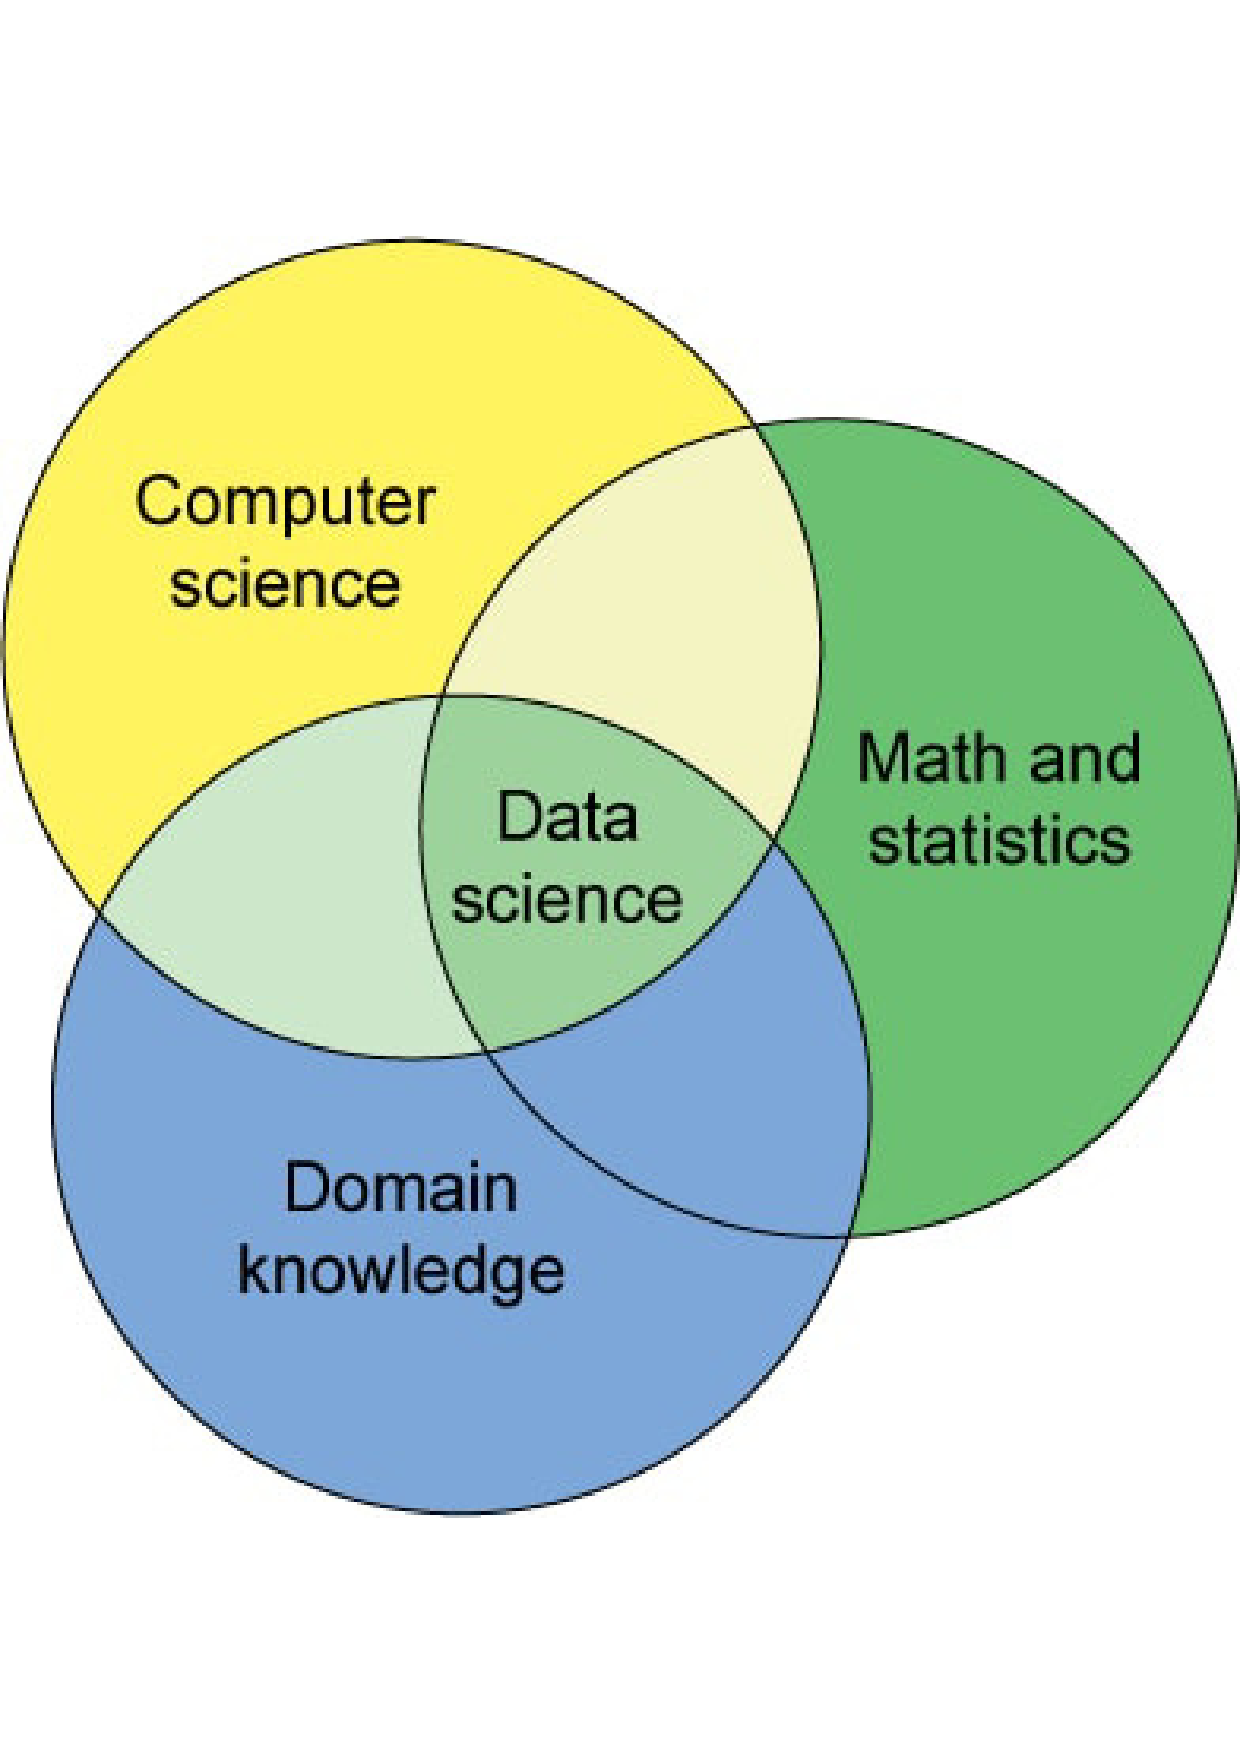
\includegraphics[trim={0 3cm 0 3cm},clip,width=0.9\textwidth]{Files/Data_Science_Concept.pdf}
    \caption{Data science concept}
    \label{fig: Data_science}
\end{figure}

\end{minipage}

\newpage 

Here is reported a short definitions about the main subdomains considered by this study:
\begin{itemize}

\item \textbf{Data mining}: Is the computing process of discovering patterns in large data sets. The overall goal of the data mining process is to extract information from a data set and transform it into an understandable structure for further use.

\item \textbf{Data Visualization}: It involves the creation and study of the visual representation of data. The primary goal of data visualization is to communication information clearly and efficiently via graphics and plots.

\item \textbf{Machine learning}: Is a subfield of computer science that, according to Arthur Samuel in 1959, gives computers the ability to learn without being explicitly programmed. More useful specific informations about this field are provided in the following section [\ref{ML}].
\end{itemize}

The follow image represents the "Blitzstein and Pfister's framework" and provides a clear overview of the Data Science process.
\begin{figure}[H]
    \centering
    \makebox[\textwidth][c]{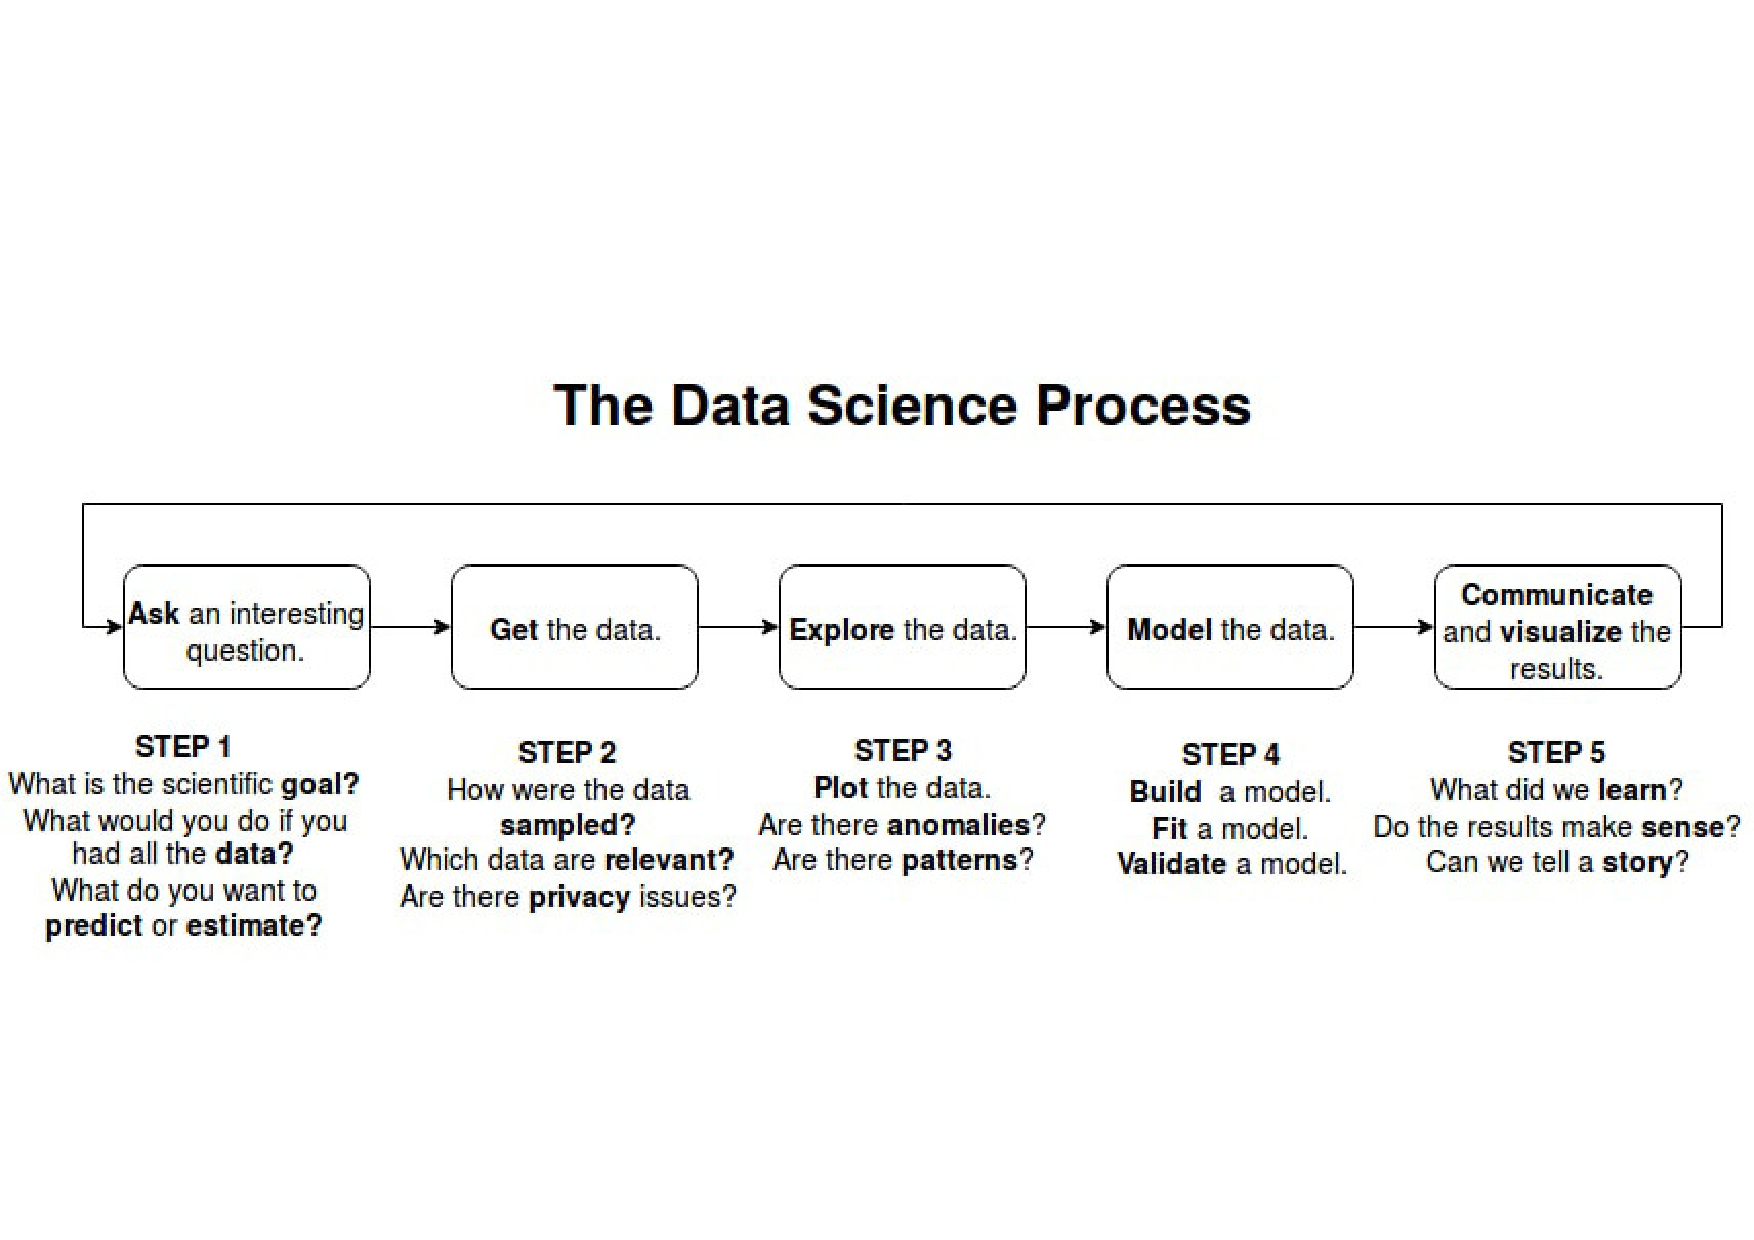
\includegraphics[trim={0 0 0 2cm},clip, width=1.2\textwidth]{Files/Data_Science_Process.pdf}}
    \caption[Data science process]{Data science process}
    \label{fig: Data_science}
\end{figure}



\newpage


\section{Machine learning}
\label{ML}
How is reported in the previous section, this subfield of computer science gives "computers the ability to learn without being explicitly programmed". \\
Machine learning explores the study and construction of algorithms that can learn from and make predictions on data.

There are several machine learning algorithm, each one of them is used for a different purpose and a different domain. For examples:
  \vspace{-5mm}
\begin{itemize}
 \setlength{\itemsep}{-5pt}
  \item Deep Learning
  \item Neural Network
  \item Regularization
  \item Clustering
  \item \textbf{Regression}: This specific domain contains the model used in this study.
  \item Bayesian
  
 \end{itemize}  

\subsection{Time Series analysis and predictions}
  \vspace{-5mm}
Time Series forecasting is an important area of machine learning, but that is often neglected. Is that important mainly beause there are so many prediction problems that involve a time component, and these problems are neglected because it is this time component that makes time series problems more difficult to handle.

" A time series is a sequence of observations taken sequentially in time. " \\
Quoted — Page 1, Time Series Analysis: Forecasting and Control.

Classic example of a time series dataset:

\begin{tabular}{ | l | l | }
\hline 		\textbf{Date}	&	\textbf{Paramater} \\ \hline
				Time \#1	&	observation \\ \hline	
				Time \#2	&	observation \\ \hline	
				Time \#3	&	observation \\ \hline											
\end{tabular}

Understanding a dataset is called time series analysis and it can helps to make better prediction, but sometimes it's not required and can result in a large of technocal investment in time and expertise.

Making predictions could be called time series forecasting and it involves taking models fit on historical data and using them to predict future observations.

\newpage 

\subsection{Autoregressive integrated moving average (ARIMA)}
\vspace{-5mm}
Since this a very complicated and deep topic, this study provided just an initial implementation and descripton of it.
During this section are provided some basic definitions and overviews enough to understand the general logic behind a forecasting system. If you are particular interested in this topic my suggestion is to read more about it, in the specific the mathematic side.\\

\textbf{AR model}: an autoregressive model is a representation of a type of random process; as such, it is used to describe certain time-varying processes in nature, economics, etc. The autoregressive model specifies that the output variable depends linearly on its own previous values and on a stochastic term (an imperfectly predictable term); thus the model is in the form of a stochastic difference equation.

\textbf{MA model}: a moving-average model is a common approach for modeling univariate time series. The moving-average model specifies that the output variable depends linearly on the current and various past values of a stochastic (imperfectly predictable) term. 

\textbf{ARMA model}: an autoregressive-moving-average model provides a parsimonious description of a stationary stochastic process in terms of two polynomials, one for the autoregression and the second for the moving average. Basically it combines both AR and MA models into a unique representation.

\textbf{ARIMA model}: is a generalization of an autoregressive moving average (ARMA) model. Both of these models are fitted to time series data either to better understand the data or to predict future points in the series (forecasting).\\
This model is applied in some cases where data show evidence of non-stationarity, where an initial differencing step (corresponding to the "integrated" part of the model) can be applied one or more times to eliminate the non-stationarity.

\textbf{ARIMA(p, d, q)}
  \vspace{-5mm}
\begin{itemize}
 \setlength{\itemsep}{-5pt}
\item \textbf{p} is the number of autoregressive terms (How many preceding values are examinated for the current value’s forecast).

\item \textbf{d} is the number of nonseasonal differences needed for stationarity.

\item \textbf{q} is the number of lagged forecast errors in the prediction equation. 
\end{itemize}

\newpage

\section{Aquaculture in Norway}

Is the aquaculture business in Norway growing? 
  
Aquaculture, also known as aquafarming, is the farming of fish, crustaceans, molluscs, aquatic plants, algae, and other aquatic organisms.

Aquaculture would be the future of fish:
In 2030, according to the World Bank, aquaculture will supply:
\begin{itemize}
\item 93.6 Million tonnes of fish per year
\item 25 percent less wild fish will be available
\item 62 percent of the fish we eat will come from farms
\end{itemize}




 % Background Theory 
%*******10********20********30********40********50********60********70********80




% For all chapters, use the newdefined chap{} instead of chapter{}
% This will make the text at the top-left of the page be the same as the chapter

\chap{Implementation Design and Requirements}
\section{System Requirements}
In the next chapters will be documented the implementation procedure for each of the system used for this study. If you want to redo the procedure or just test the final resulting system, it's important to follow the right requirements.

\subsection{Requirements for reusability}
\vspace{-5mm}
Both the analysis systems that are going to be implemented during this phase of the work will need for just one requirement about the input dataset:
\vspace{-5mm}
\begin{itemize}
\item Monthly frequency of data values.
\end{itemize}

\subsection{System requirements}
\vspace{-5mm}
It's important to remind that this proceure will describes the system implentation using Python, so be sure to have installed all the necessary for compile and execute Python code on your platform. Current development environment:
\begin{lstlisting}
Python version: 2.7.12
\end{lstlisting}
\vspace{-5mm}
It's also necessary to have installed the following Python libraries:
\vspace{-5mm}
\begin{itemize}
\setlength{\itemsep}{-5pt}
\item  SciPy \footnote{SciPy : \url{https://www.scipy.org/install.html}}
\item Cartopy \footnote{Cartopy : \url{http://scitools.org.uk/cartopy/docs/latest/installing.html\#installing}}
\end{itemize}



\newpage

\section{System Design}
\label{System_Design}
How written above in the Thesis Structure section \ref{Thesis_Strucutre}, the implemented Python system has been divided in different subsystems. This decision was taken because the system has to implement functions and utilities that are quite different between them, so split it in subsytems allows to maintain the reusability and increase the understanding of the implemented code.
The following figure and text provide a general idea about the systems that are implemented during this study.

\begin{figure}[h]
    \makebox[\textwidth][c]{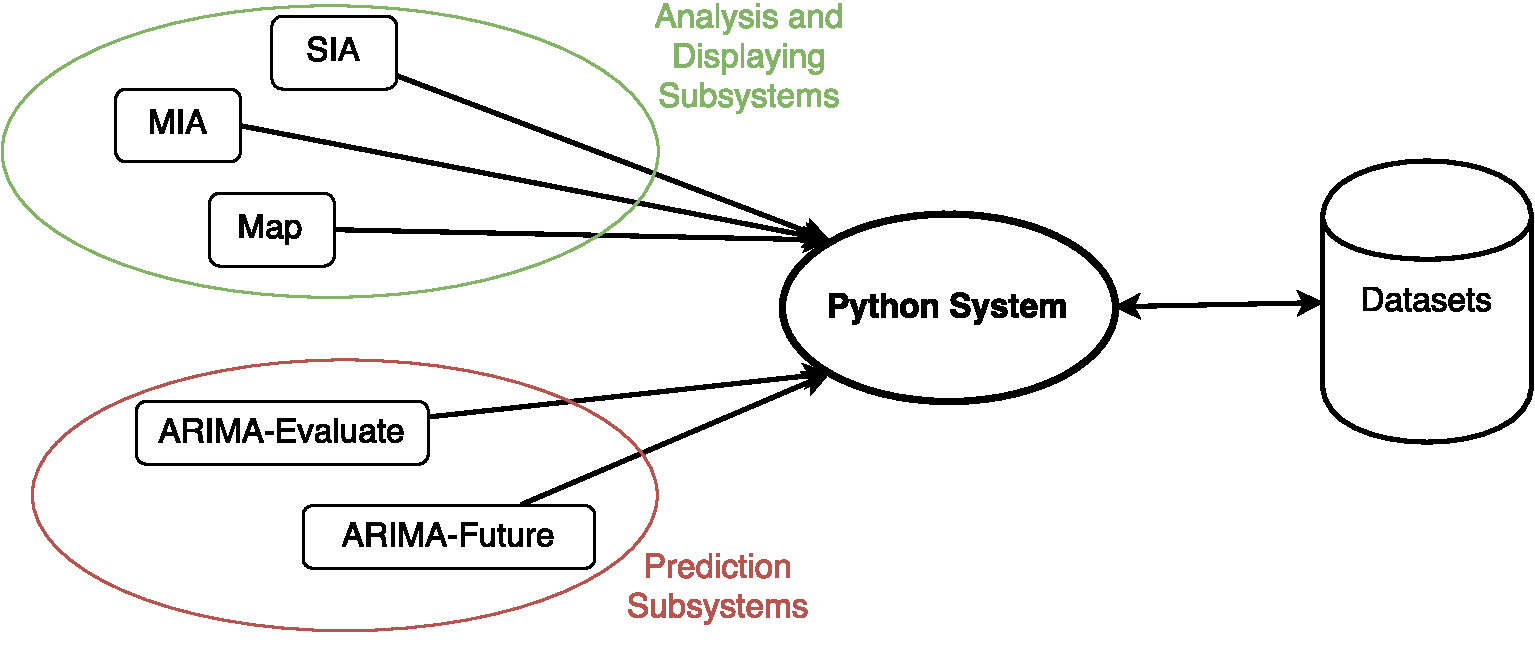
\includegraphics[width=1\textwidth]{Files/SystemDesign.pdf}}
    \caption[Subsystems overview]{Subsystems overview.}
    \label{fig: Subsystems_Overview}
\end{figure}

\vspace{-5mm}
\begin{itemize}
 %\setlength{\itemsep}{-5pt}
 \item \textbf{Single Input Analyzer (SIA)}: Will provide the analysis results about a specific parameter of the input dataset.
 \item \textbf{Multiple Input Analyzer (MIA)}: Will provide the analysis result about all the parameters of the input dataset, such as the correlation between, comparisons,.. 
 \item \textbf{Map}: Will provide a data visualization able to display some of the data on a Norway's territory map.
 \item \textbf{ARIMA-Evaluate}: Will provide a system able to evaluation different configurations of an ARIMA machine about a specific paramater of the current input dataset.
 \item \textbf{ARIMA-Future}: Will provide a system able to get some future predictions about a parameter of the current input dataset using a specific configuration of the ARIMA machine, that should be the best one obtained during the Evaluation process.
\end{itemize} 



 % Approach and Design

%
\chap{Implementation}

\hypersetup{
    colorlinks=true,
    linkcolor=blue,
    filecolor=magenta,      
    urlcolor=blue,
}

\DeclareFixedFont{\ttb}{T1}{txtt}{bx}{n}{12} % for bold
\DeclareFixedFont{\ttm}{T1}{txtt}{m}{n}{12}  % for normal
\definecolor{deepblue}{rgb}{0,0,0.5}
\definecolor{deepred}{rgb}{0.6,0,0}
\definecolor{deepgreen}{rgb}{0,0.5,0}

% Python style for highlighting
\lstset{
	backgroundcolor = \color{Ivory},
    language=Python,
    basicstyle=\footnotesize,
    otherkeywords={self},             
    keywordstyle=\footnotesize\color{deepblue},
    emph={__init__},          
    emphstyle=\footnotesize\color{deepred},    
    stringstyle=\color{deepgreen},
    frame=single,                         
    showstringspaces=false  ,
    breaklines=true,
    numbers=left,
    numberstyle=\footnotesize,
    tabsize=3,
    breakatwhitespace=false
}


\subsection{Implemented Systems repositories}
The system that is going to be implemented during this thesis can be easily downloaded in order to test it and better understandhow it works.\\
The github repository of the implementation is the following:\\
\url{https://github.com/Sprea22/Norway_County_Analyzer}\\
Direct link for the already implemented Data Analyzer in Python.\\
\url{https://codeload.github.com/Sprea22/Data_Analyzer_Python/zip/master}\\

\url{https://github.com/Sprea22/Forecasting_System_Python}\\
Direct link for the already implemented Forecasting System in Python.\\
\url{https://codeload.github.com/Sprea22/Forecasting_System_Python/zip/master}





	 % Implementation

\part{Data Collection and Validation}

\newpage
\chapter{Data Sources and Elaboration}
\section{Data Sources}
The collection of the data has been an important phase during this work. \\
Several sources have been checked and consulted in order to find reliable and useful data for the final purpose of this thesis. In this particular case, the main data collection way was internet, but some important data have been provided also from SINTEF Nord.
\citation{}

\subsection{Data from SINTEF Nord}
Some of the data used during this thesis were provided from the members of the eSushi project at SINTEF Nord.
The origin source of the data is "Archieve Norstore"\footnote{Source link for data downloaded by Archieve Norstore: \\\url{https://archive.norstore.no/pages/public/datasetDetail.jsf?id=10.11582/2015.00014}}, which allows to anyone to download published just providing a valid email address \footnote{"6.1 Download a public dataset" : \\ \url{https://archive.norstore.no/user-guide.pdf}}. 

The data are about each single Norwegian county with the following details:\\

\begin{table}[ht]
\makebox[\textwidth][c]{
\resizebox{1\textwidth}{!}{
    \begin{tabular}{ | l | l | l | l | l |}
            \hline \textbf{Input}	&	\textbf{Content}	& \textbf{Unit}  & \textbf{Frequency}  & \textbf{Available Period} \\ \hline
\multicolumn{1}{|p{4cm}|}{\raggedright 1. Average Sea Temperature}	&	
\multicolumn{1}{p{4cm}|}{\raggedright Reported number of cages with salmon and rainbow trout.}
								& Celsius & Monthly & January 2007 - April 2014 	\\ \hline	
\end{tabular}}}
    \caption{Data provided from SINTEF Nord. }
    \label{table: SINTEF_Data} 
\end{table}



\newpage
 
\subsection{Data from Fiskeridirektoratet} 
Fiskeridirektoratet\footnote{Source link for data downloaded by Fiskeridir: \\ \url{http://www.fiskeridir.no/Akvakultur/Statistikk-akvakultur/Biomassestatistikk}} has been the main data source for this work. They provide several statistics about Aquaculture in Norway which are subject to the Norwegian Public Data License (NLOD), that allows a free reusage of the data on the terms developed by Difi \footnote{Terms of use of the Directorate of Fisheries's data (Difi): \\ \url{http://data.norge.no/nlod/no}}.\\
The data inputs from the current website used for this thesis are reported below, and they are available for each single county in Norway involved in Aquaculture business:

\begin{table}[ht]
\makebox[\textwidth][c]{
\resizebox{1\textwidth}{!}{
    \begin{tabular}{ | l | l | l | l | l |}
            \hline
\textbf{Input}							&	\textbf{Content}	& \textbf{Unit} & \textbf{Frequency} & \textbf{Available Period} \\ \hline
1. Cages							&	\multicolumn{1}{p{4cm}|}{\raggedright Reported number of cages with salmon and rainbow trout.}
									& Number & Monthly & January 2005 - April 2017 	\\ \hline									
2. Localities						& \multicolumn{1}{p{4cm}|}{\raggedright Reported number of localities with salmon and rainbow trout.}
									& Number & Monthly & January 2007 - April 2017 \\ \hline
3. Feed consumption	&  \multicolumn{1}{p{4cm}|}{\raggedright Reported feed consumption for Salmon.}		
									& Tonnes & Monthly & January 2007 - April 2017  	\\ \hline
4. Restock			& \multicolumn{1}{p{4cm}|}{\raggedright Fish restock reported for Salmon.}	
									& 1000 pcs & Monthly & January 2007 - April 2017 	\\ \hline
5. Withdrawals 			& \multicolumn{1}{p{4cm}|}{\raggedright Withdrawals of Salmon for slaughter. } 		
									& Tonnes & Monthly & January 2007 - April 2017  	\\ \hline
6. Biomass		& \multicolumn{1}{p{4cm}|}{\raggedright Reported biomass of Salmon. }
									& Tonnes & Monthly & January 2007 - April 2017  \\ \hline
7. Salmon Number 		& \multicolumn{1}{p{4cm}|}{\raggedright Reported number of Salmon. }		
									& Number & Monthly & January 2007 - April 2017  \\ \hline
    \end{tabular}}}\\
     \caption{Data provided from Fiskeridirektoratet.}
    \label{table: Fiskeridir_Data} 
\end{table}  
    
About the current data source it is also important to know that:
\begin{itemize}
\item The data are available from 2005 to 2017.
\item The data are uploaded once per month.
\item The data are reported and available just in XLSX format.
\item The data are available just in Norwegian.
\item It is not possible to implement an automatic download script.
\end{itemize}

\newpage


\subsection{Data from Indexmundi} 
An another source of data for this study was Indexmundi\footnote{Source link for data downloaded by Indexmundi: \\ \url{http://www.indexmundi.com/commodities/?commodity=fish}}, which provides data about fish (salmon) monthly price, Norwegian krone per kg, with a public access policy.\\

\begin{table}[ht]
\makebox[\textwidth][c]{
\resizebox{1\textwidth}{!}{
    \begin{tabular}{ | l | l | l | l | l |}
            \hline
\textbf{Input}	 &	\textbf{Content}	& \textbf{Unit} & \textbf{Frequency} & \textbf{Available Period} \\ \hline
\multicolumn{1}{|p{4cm}|}{\raggedright 1. Export Salmon Price}	&	
\multicolumn{1}{p{4cm}|}{\raggedright Reported farm bred Norwegian Salmon export price.}
									& NOK/KG & Monthly & January 2005 - April 2017 	\\ \hline	
\end{tabular}}}									
     \caption{Data provided from Indexmundi.}
    \label{table: Indemundi_Data} 
\end{table}  

\section{Increase accessibility and availability of data}
In order to increase the accessibility and availability of the downloaded data, during this phase the main goals were:
\vspace{-2mm}
\begin{itemize}
 \setlength{\itemsep}{-5pt}
\item Provide an accurate description in English language, since most of the data were available just in Norwegian.
\item Report the data in a standard and reusable format (CSV).
\item Design and build a easily readable dataset structure.
\end{itemize} 

The final decision about the datasets set up during this thesis provided the followng list of datasets, where the structure can be checked in the following two pages.
\vspace{-2mm}
 \setlength{\itemsep}{-5pt}
\begin{itemize}
\item Overview Dataset: Norway.csv
\vspace{-2mm}
\item County 1 Dataset: Finnmark
\vspace{-2mm}
\item County 2 Dataset: Troms
\vspace{-2mm}
\item County 3 Dataset: Nordland
\vspace{-2mm}
\item County 4 Dataset: Nord Trondelag
\vspace{-2mm}
\item County 5 Dataset: Sor Trondelag
\vspace{-2mm}
\item County 6 Dataset: More og Romsdal
\vspace{-2mm}
\item County 7 Dataset: Sogn og Fjordane
\vspace{-2mm}
\item County 8 Dataset: Hordaland
\vspace{-2mm}
\item County 9 Dataset: Rogaland og Agder
\end{itemize}

\newpage

\subsection{Dataset about Norway}

\begin{figure}[H]
        \makebox[\textwidth][c]{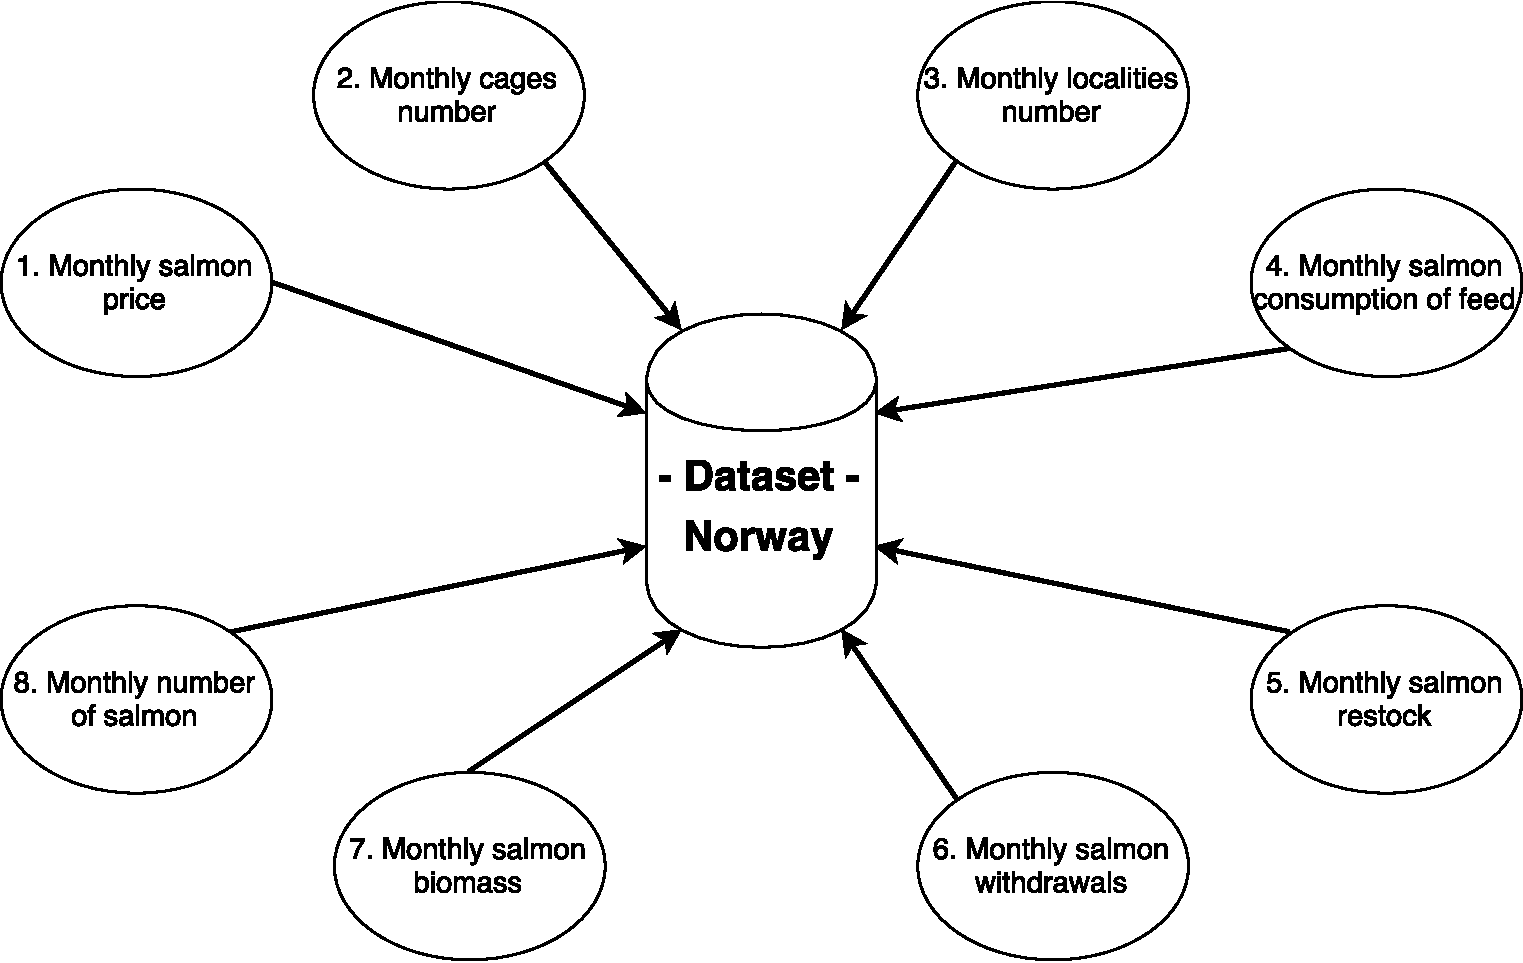
\includegraphics[width=1\textwidth]{Files/Dataset.pdf}}
    \caption{Dataset structure.}
\end{figure}

\begin{table}[ht]
\makebox[\textwidth][c]{
\resizebox{1\textwidth}{!}{
    \begin{tabular}{ | l | l | l | l | }
            \hline
\textbf{Input}						& \textbf{Frequency} & \textbf{Period} & \textbf{Location}	\\ \hline
1. Export Salmon Price				& Monthly 			& January 2005 - December 2016 		& Norway 	\\ \hline	
2. Cages							& Monthly 			& January 2005 - December 2016 		& Norway 	\\ \hline									
3. Localities						& Monthly 			& January 2005 - December 2016 		& Norway	\\ \hline
4. Feed consumption					& Monthly 			& January 2005 - December 2016 		& Norway  	\\ \hline
5. Restock							& Monthly 			& January 2005 - December 2016 		& Norway	\\ \hline
6. Withdrawals 						& Monthly 			& January 2005 - December 2016 		& Norway 	\\ \hline
7. Biomass							& Monthly 			& January 2005 - December 2016 		& Norway 	\\ \hline
8. Salmon Number 					& Monthly 			& January 2005 - December 2016 		& Norway	\\ \hline
    \end{tabular}}}
         \caption{Structure of the dataset about Norway.}
    \label{table: Norway_Dataset_struc} 
\end{table}  


\subsection{Dataset about single county} 

\begin{figure}[H]
        \makebox[\textwidth][c]{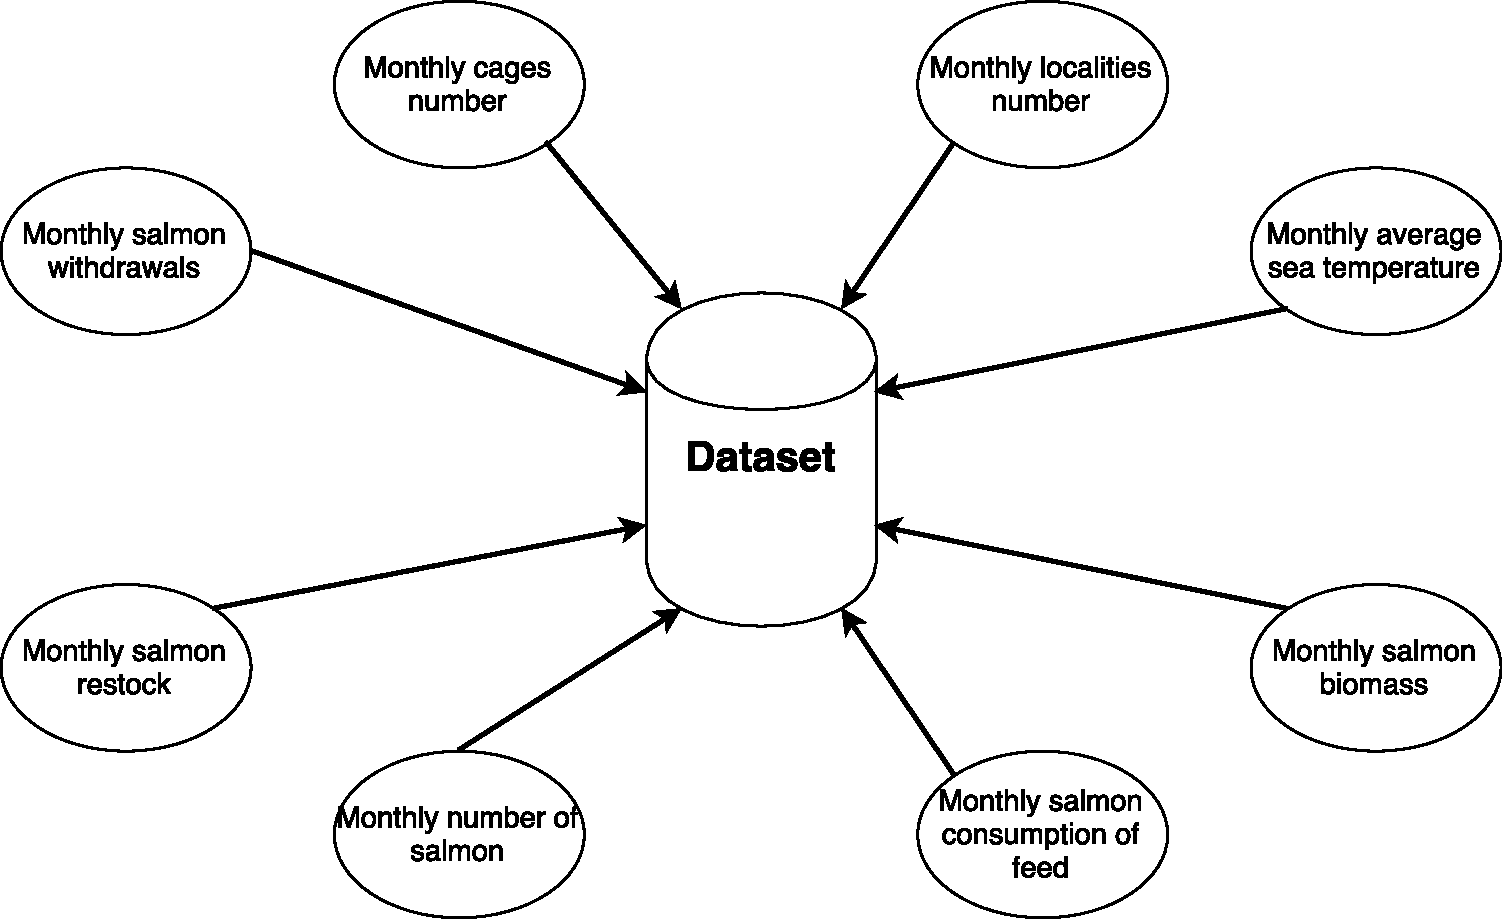
\includegraphics[width=1\textwidth]{Files/Dataset2.pdf}}
    \caption{Dataset structure.}
\end{figure}

The dataset that contains data about a single county has a shorter availability period of the values than the dataset about Norway, that is because of the sea average temperature values that have shorter range compared with the other inputs (2007-2014 instead of 2005-2016).

\begin{table}[ht]
\makebox[\textwidth][c]{
\resizebox{1\textwidth}{!}{
    \begin{tabular}{ | l | l | l | l | }
            \hline
\textbf{Input}						& \textbf{Frequency} & \textbf{Period} & \textbf{Location}	\\ \hline
1. Average Sea Temperature				& Monthly 			& January 2007 - December 2014 		& Single county 	\\ \hline	
2. Cages							& Monthly 			& January 2007 - December 2014 		& Single county 	\\ \hline									
3. Localities						& Monthly 			& January 2007 - December 2014 		& Single county	\\ \hline
4. Feed consumption					& Monthly 			& January 2007 - December 2014 		& Single county  	\\ \hline
5. Restock							& Monthly 			& January 2007 - December 2014 		& Single county	\\ \hline
6. Withdrawals 						& Monthly 			& January 2007 - December 2014 		& Single county 	\\ \hline
7. Biomass							& Monthly 			& January 2007 - December 2014 		& Single county 	\\ \hline
8. Salmon Number 					& Monthly 			& January 2007 - December 2014 		& Single county	\\ \hline
    \end{tabular}}}
         \caption{Structure of the dataset about each norwegian county.}   
   \label{table: County_dataset_struc} 
\end{table}      

\part{Implementation}

\chapter{Analyzer System}

Total implementation link for data analyzer : \\
\url{https://github.com/Sprea22/Python_Systems}

During this part the main purpose is to analyze the whole dataset in order to find some kind of useful informations later on. 

The system that it's going to be implemented during this part of the work could be divided in two subsystems, with the relative outcomes:
\begin{itemize}
\item Single Input Analyzer (SIA): Used for analyze a single data input.
\begin{itemize}
\item Total graphic of the input data for the whole period.
\item Graphic of the input data for each single year.
\item Correlation matrix between different months of the same input.
\item Correlation matrix between different years of the same input.
\end{itemize}
\item Multiple Inputs Analyzer (MIA): Used for analyze multiple data inputs.
\begin{itemize}
\item General correlation matrix between all the different inputs.

\item Graphic of the normalized angular coefficients of all the inputs.
\end{itemize}
\end{itemize}

\newpage


\section{Single Input Analyzer}
It's possible to check out the total implementation code of the SIA in the appendice  [\ref{SIA_Implementation}].
The implementation of this Analyzer can be divided in the following parts:
\begin{itemize}
\item SIA imported libraries. 
\item SIA part I: Generate and display a graphic about current input with total data.
\item SIA part II: Generate and display a graphic about current input for each year.
\item SIA part III: Generate and display a graphic that contains the correlation matrix between each single year of the current input.
\item SIA part IV: Generate and display a graphic that contains the correlation matrix between each single months of the year of the current input.
\item SIA part V: Generate and display a single overview image for the current input.
\end{itemize}

\subsection{SIA: Imported libraries}
Specific Python libraries have been imported for the implementation of this system.
It's possible to find out a list of this libraries with a specific description for each of them in the appendice [\ref{SIA_libraries}].

\newpage

\subsection{SIA section I: Total graphic for all the years}
\textbf{Goal:}\\
Generate and display the total graphic about current input, and then calculate and display the trend line as well. Trend line angular coefficient has to be save in a document.

\textbf{Requirements:}\\
The current data input has to be with a monthly frequency. 

\textbf{Implementation:}\\
To reach the current goal have been used two main functions of the "pandas" library. They allow to read the data values from the dataset and display it on a graphic.
\begin{lstlisting}
series = pandas.read_csv()
seris.plot()
\end{lstlisting}

It's possible to check out the full commented implementation in the appendice: [\ref{SIA_section_I}]

\textbf{Results:} \\
With this first part of the code has been reached the first goal of displaying and saving the basic graphic about the current input, with also the relative trend line and saving it angular coefficient in a document, that looks like:

\begin{figure}[H]
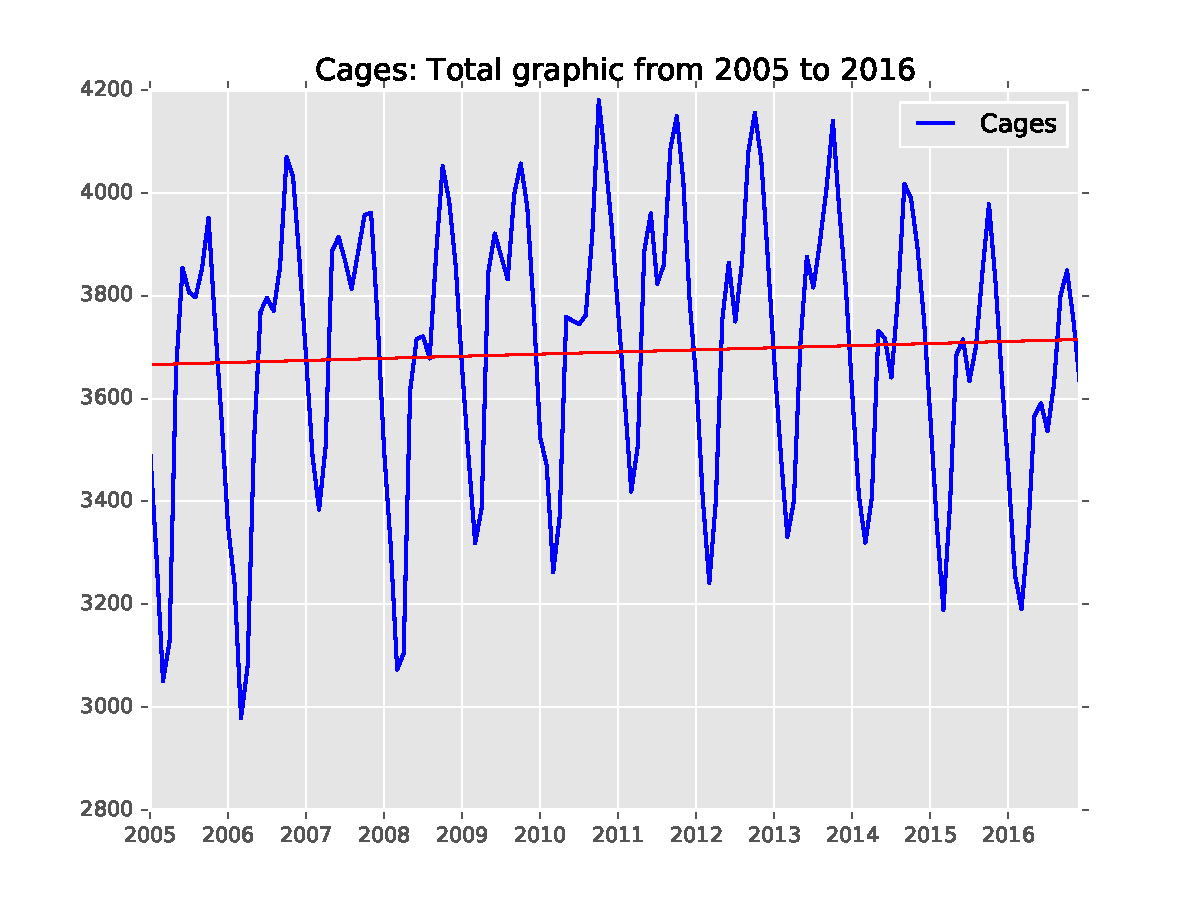
\includegraphics[width=0.9\textwidth]{Files/Cages_Total.pdf}
\caption{Total graphic about current input over the whole period.}
\end{figure}



\newpage
\subsection{SIA section II: Single graphics for each year}

\textbf{Goal:}\\
Generate and display a graphic that contains the plots of each single year over the whole period of the current input. 

\textbf{Requirements:}\\
The current data input has to be with a monthly frequency. 

\textbf{Implementation:}\\
To reach the current goal have been used two main libraries.\\
The "pandas" library allows to read the data values from the dataset and return it like "ndarray" type, then the library "pyplot" allows to display it on a graphic.
\begin{lstlisting}
series = pandas.read_csv()
series.values()
pyplot.plot()
\end{lstlisting}

It's possible to check out the full ccommented code in the appendice: [\ref{SIA_section_II}]

\textbf{Results:} \\
With this second part of the code has been reached the goal of displaying and saving the graphic of the plots for each single year of the current input, that looks like:
\begin{figure}[H]
	\centering
    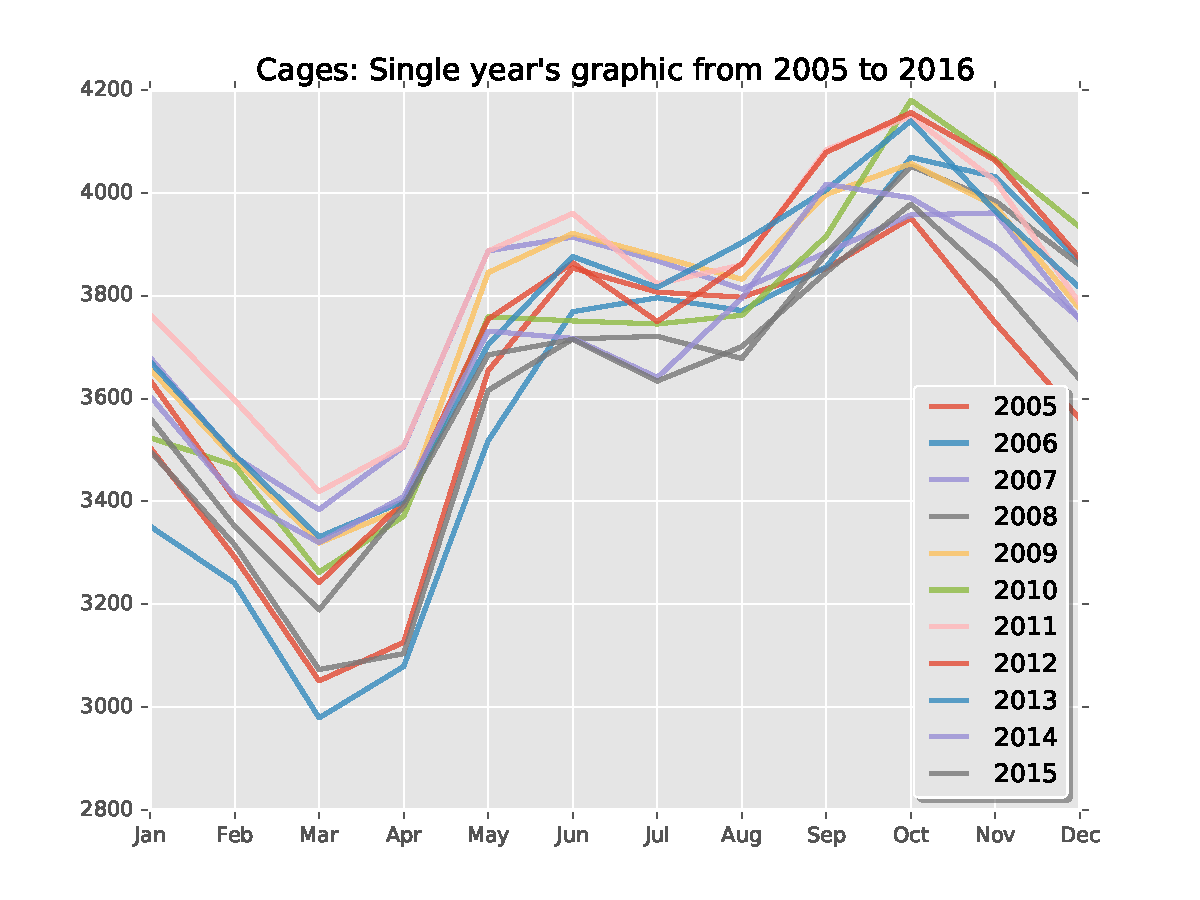
\includegraphics[width=0.9\textwidth]{Files/Cages_Years.pdf}
    \caption{Graphics for each single year of the current input data.}
\end{figure}




\newpage
\subsection{SIA section III: Correlation matrix between years}

\textbf{Goal:}\\
Calculate and save the correlation coefficients between each single year over the whole period of the current input and then display it with a correlation matrix.

\textbf{Requirements:}\\
The current data input has to be with a monthly frequency. 

\textbf{Implementation:}\\
To reach the current goal have been used the scientific computing library "numpy", that allows to calculate the correlation coefficients between data. Then the library "pyplot" has been used to display the results on a matrix.
\begin{lstlisting}
numpy.corrcoef()
figure = pyplot.figure()
ax = figure.add_subplot()
ax.matshow()
\end{lstlisting}

It's possible to check out the full ccommented code in the appendice: [\ref{SIA_section_III}]

\textbf{Results:} \\
With this part of the code have been calculated and displayed the correlation coefficients between each single year of the current input, that looks like:

\begin{figure}[H]
	\centering
    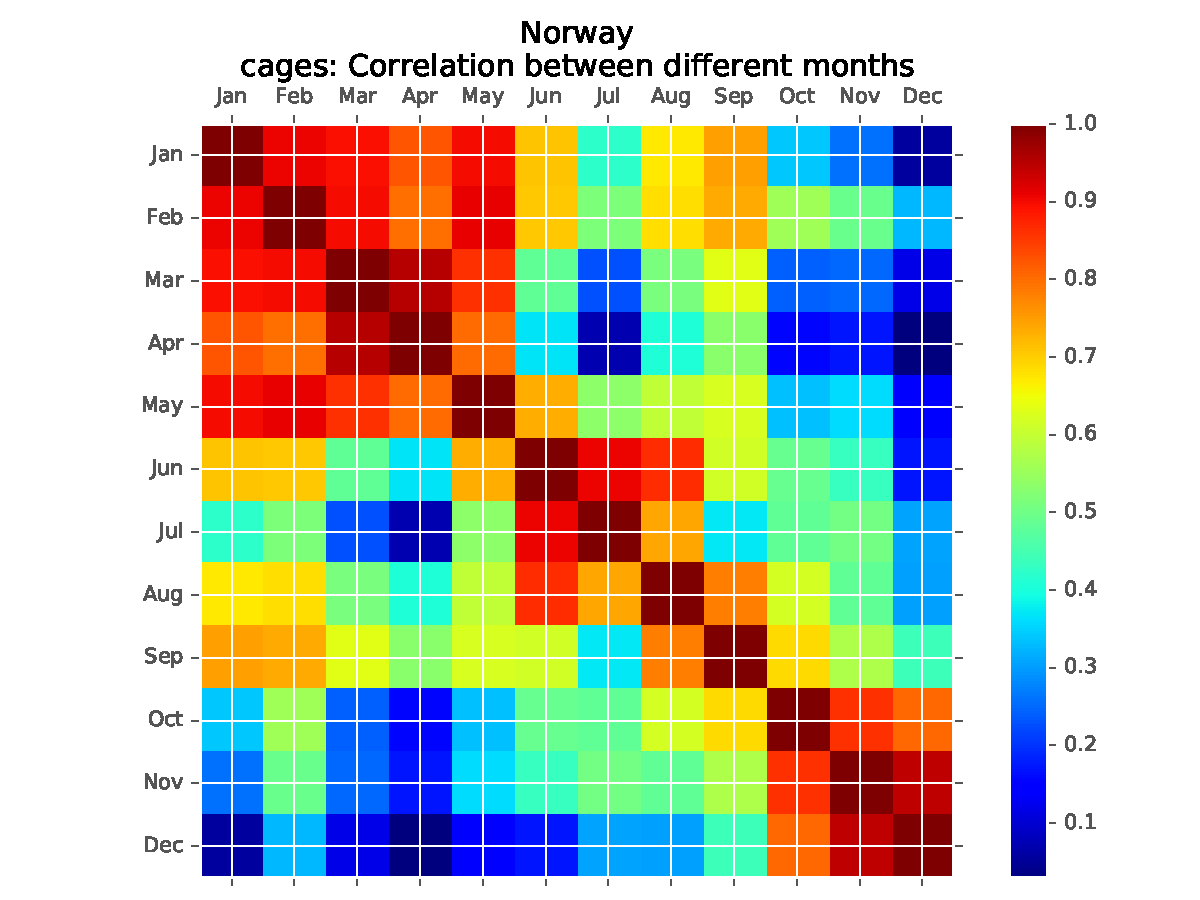
\includegraphics[width=0.9\textwidth]{Files/Cages_Months_Matrix.pdf}
    \caption{Correlation matrix between different months of the same input}
\end{figure}




\newpage
\subsection{SIA section IV: Correlation matrix between months}

\textbf{Goal:}\\
Calculate and save the correlation coefficients between each single month of the current input and then display it with a correlation matrix.

\textbf{Requirements:}\\
The current data input has to be with a monthly frequency. 

\textbf{Implementation:}\\
To reach the current goal have been used the scientific computing library "numpy", that allows to calculate the correlation coefficients between data. Then the library "pyplot" has been used to display the results on a matrix.

\begin{lstlisting}
numpy.corrcoef()
figure = pyplot.figure()
ax = figure.add_subplot()
ax.matshow()
\end{lstlisting}

It's possible to check out the full ccommented code in the appendice: [\ref{SIA_section_IV}]


\textbf{Results:} \\
With this part of the code have been calculated and displayed the correlation coefficients between each single month of the current input, that looks like: 

\begin{figure}[H]
	\centering
    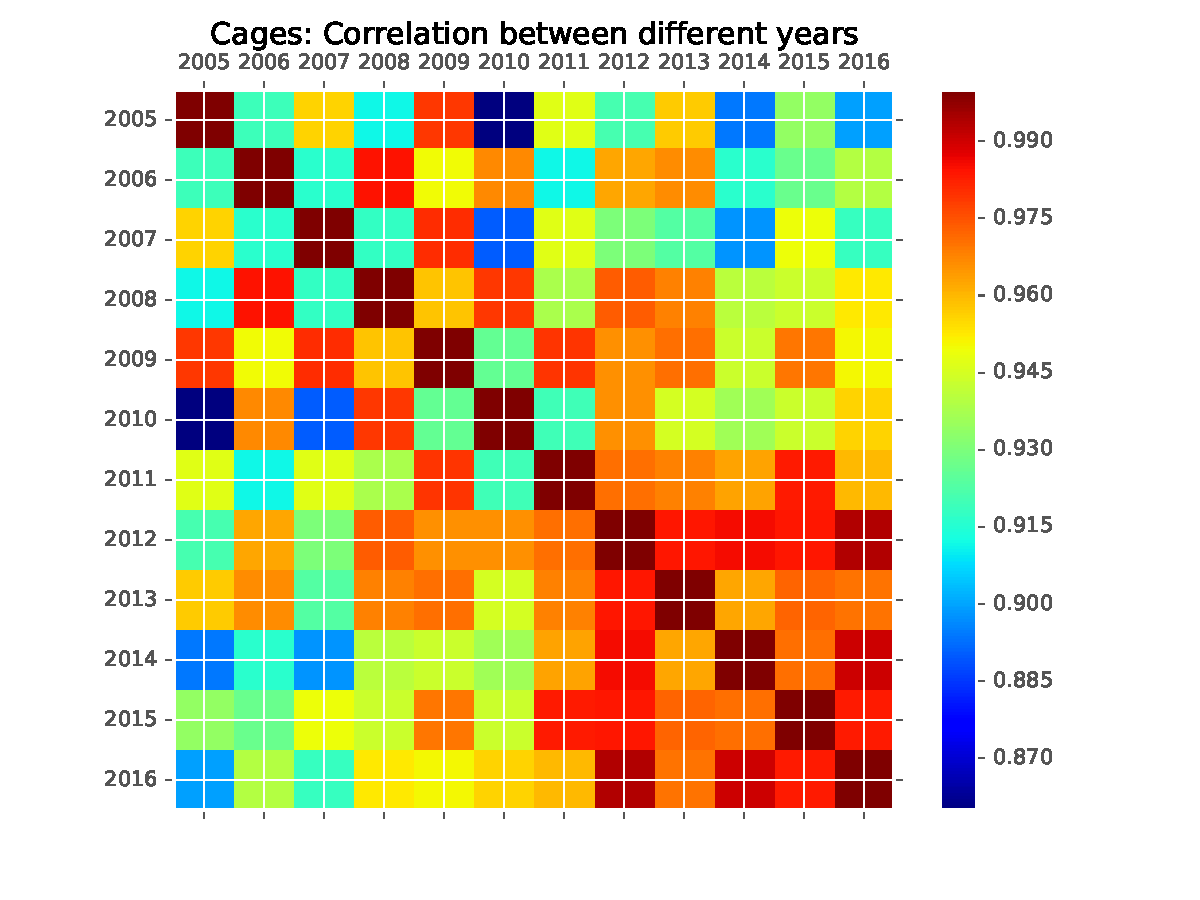
\includegraphics[width=0.9\textwidth]{Files/Cages_Years_Matrix.pdf}
    \caption{Correlation matrix between different years of the same input}
\end{figure}


\newpage
\subsection{SIA section V: Single overview}

\textbf{Goal:}\\
Generate and display a single overview image that contains all the graphics previous calculated about the current input.

\textbf{Requirements:}\\
All the graphics about the current input have to be already calculated and saved.

\textbf{Implementation:}\\
During this part of the implemented system has been indispensable the Python Imaging Library, called also PIL. 
\begin{lstlisting}
from PIL import Image
\end{lstlisting}

It basically allowed to create a new "empty" image and then create a sort of collage pasting the already calculated graphic's images on it.
\begin{lstlisting}
new_im = Image.new()
new_im.paste()
\end{lstlisting}

The following method contains the full code that allows to create the overview image. 
\begin{lstlisting}
def create_single_overview(cols, rows, dest, width, height, listofimages):
\end{lstlisting}
The output of this phase depends by the input to this method, that are basically the list of image and the preferences about the collage's structure.\\
Is possible to view the final result of this phase in the next page and is possible to check out the full ccommented code in the appendice: [\ref{SIA_section_V}]

\newpage

\textbf{Results:}\\
With this part of the code it's possible to have a single overview image about the current input, that basically allows to compare all the graphics already calculated about this input. The general overview graphic contains:
\begin{itemize}
\item Total graphic of the input data for the whole period.
\item Graphic of the input data for each single year.
\item Correlation matrix between different months of the same input.
\item Correlation matrix between different years of the same input.
\end{itemize}

\begin{figure}[H]
\begin{subfigure}{.5\textwidth}
	\centering
    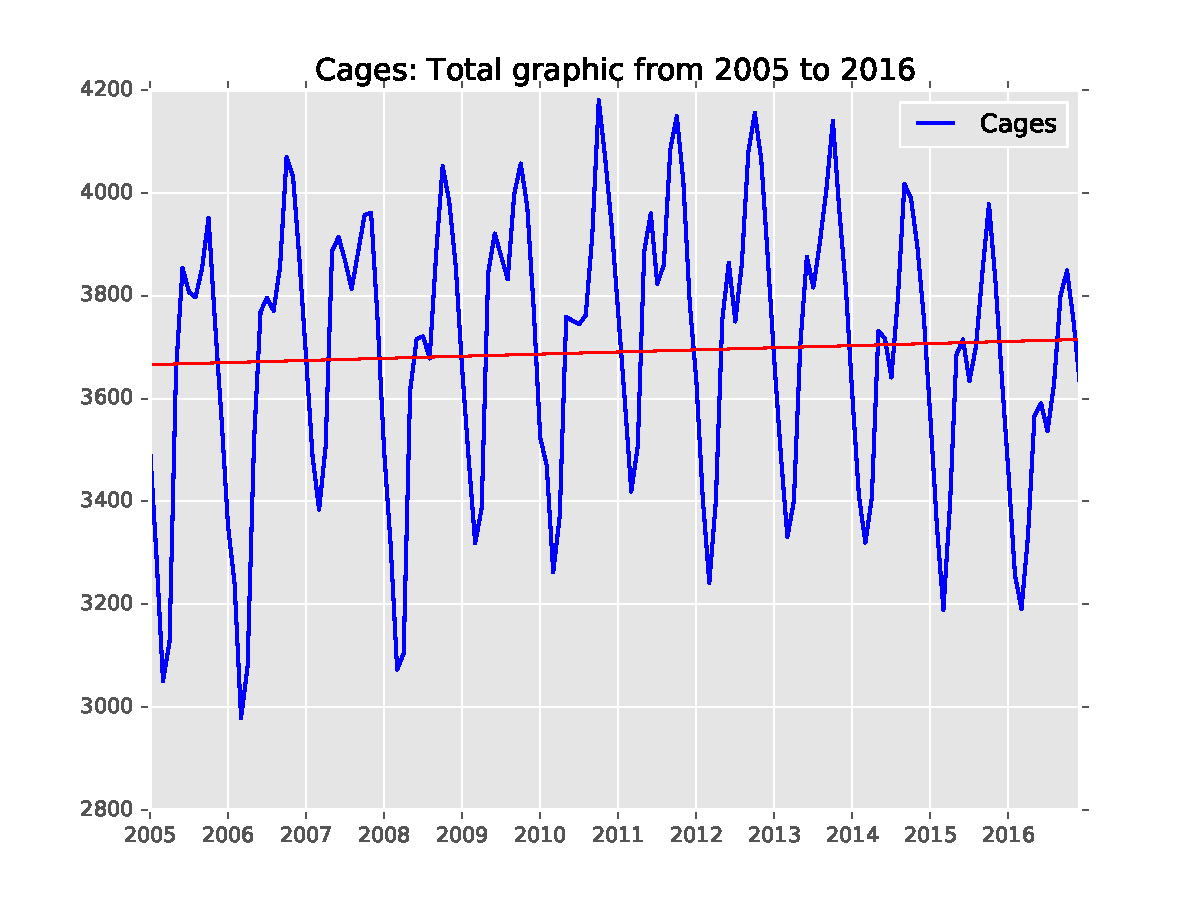
\includegraphics[width=1\textwidth]{Files/Cages_Total.pdf}
\end{subfigure}%
\begin{subfigure}{.5\textwidth}
	\centering
    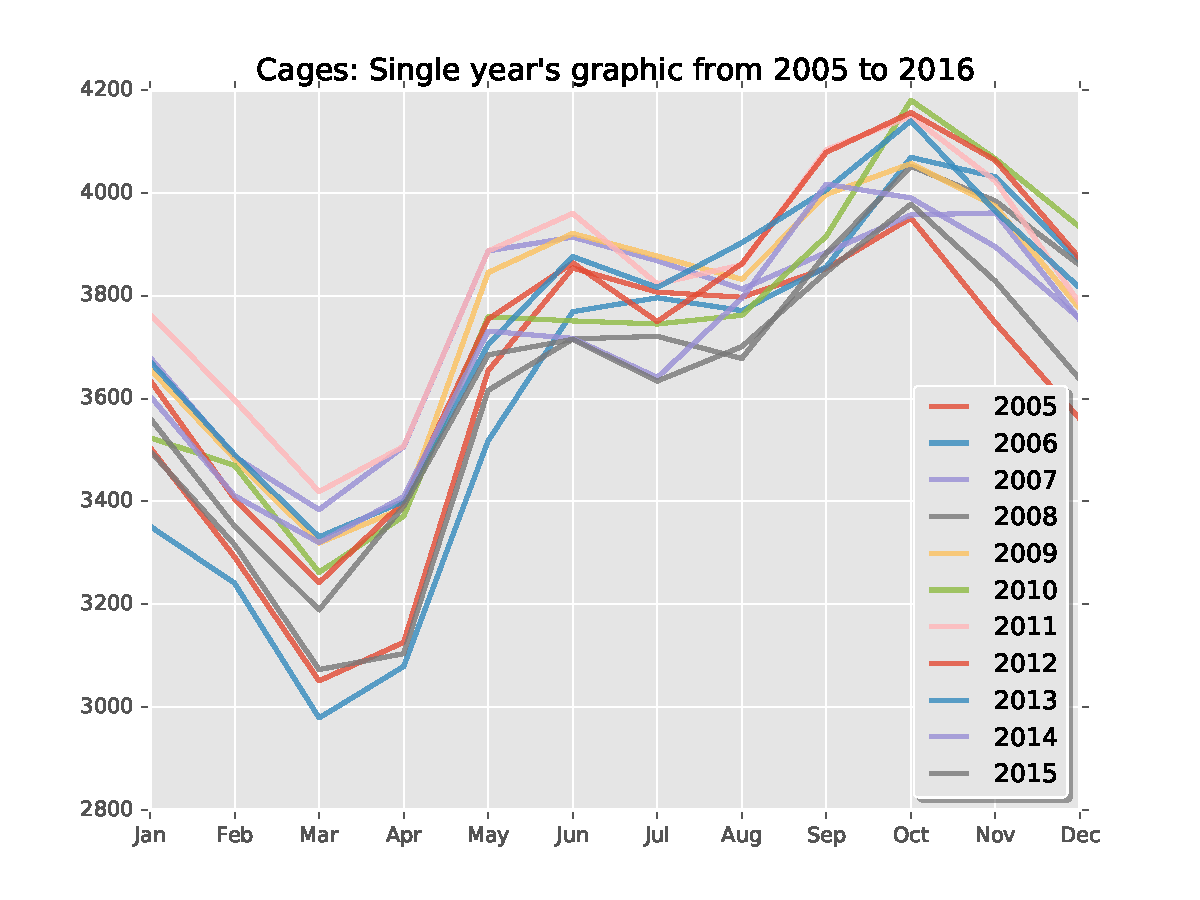
\includegraphics[width=1\textwidth]{Files/Cages_Years.pdf}
\end{subfigure}%
\end{figure} 

\begin{figure}[H]
\begin{subfigure}{.5\textwidth}
	\centering
    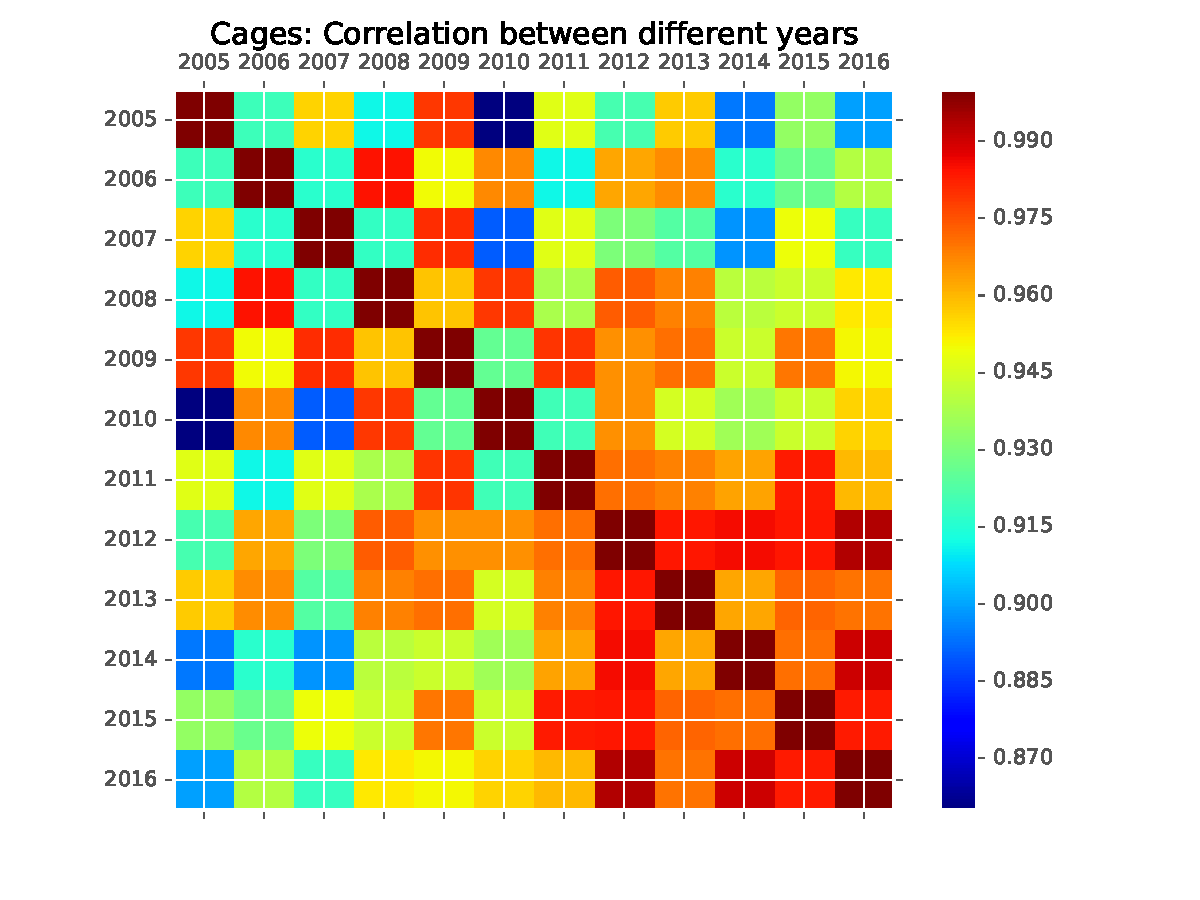
\includegraphics[width=1\textwidth]{Files/Cages_Years_Matrix.pdf}
\end{subfigure}%
\begin{subfigure}{.5\textwidth}
	\centering
    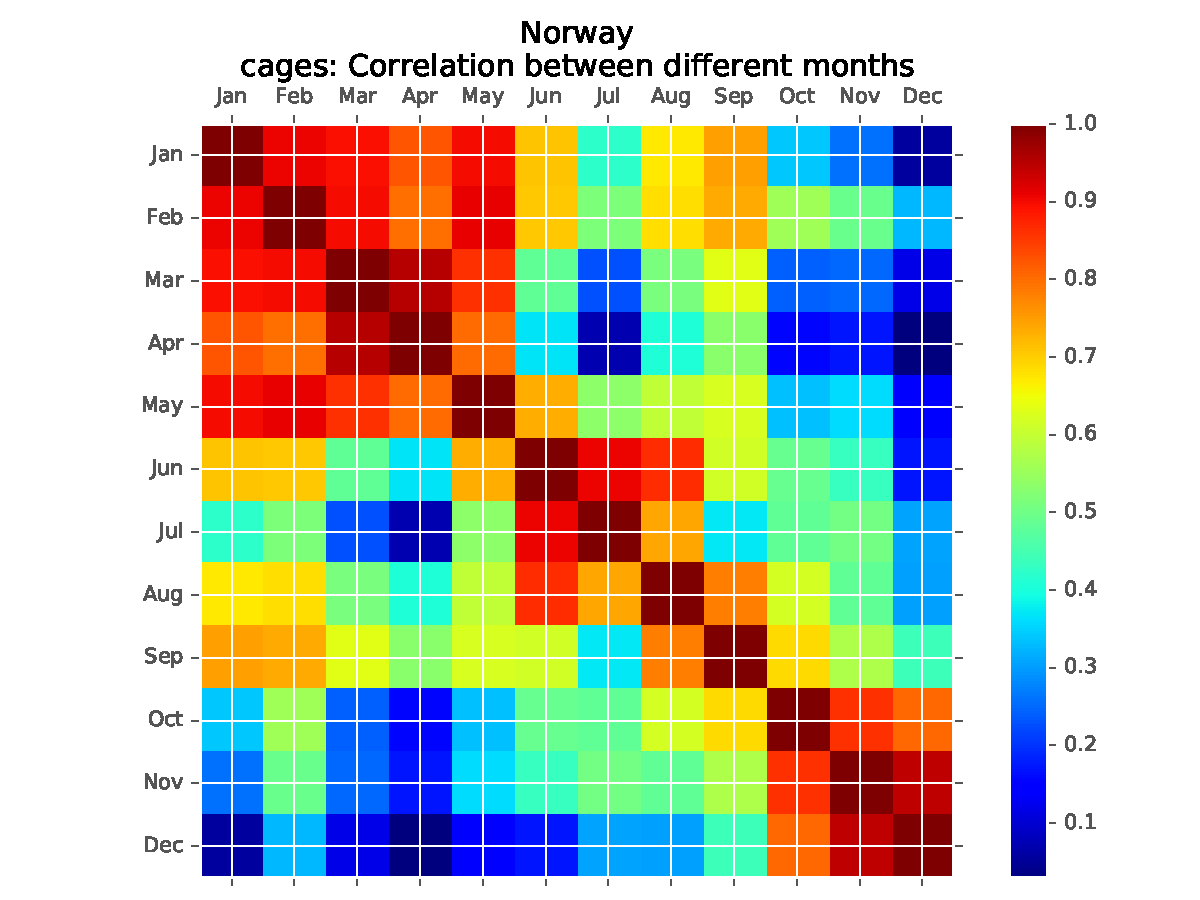
\includegraphics[width=1\textwidth]{Files/Cages_Months_Matrix.pdf}
\end{subfigure}%
\end{figure}

\newpage

\section{Multiple Inputs Analyzer}
The implementation of this Analyzer can be divided in the following parts:
\begin{itemize}
\item MIA imported libraries. 
\item MIA part I: Calculate the correlation coefficients between the different input of a dataset, save the result and display it in a matrix.
\item MIA part II: Display the comparison graphic between the different input's trend line normalized angular coefficients.
\end{itemize}

It's possible to check out the total implementation of the MIA in the appendice  [\ref{MIA_Implementation}].

\subsection{MIA: Imported libraries}
Specific Python libraries have been imported for the implementation of this system.
It's possible to find out a list of this libraries with a specific description for each of them in the appendice [\ref{MIA_Libraries}].

\newpage

\subsection{MIA section I: Total Correlation Coefficients}
\textbf{Goal:}\\
Calculate and save the correlation coefficients between different inputs of the current dataset and then show it with a matrix.

\textbf{Requirements:}\\
To let the MIA system works in a proper way, is necessary that the current dataset has been already analyzed from the SIA system.

\textbf{Implementation:}\\
To reach the current goal have been used the scientific computing library "numpy", that allows to calculate the correlation coefficients between data. Then the library "pyplot" has been used to display the results on a matrix.
\begin{lstlisting}
numpy.corrcoef()
figure = pyplot.figure()
ax = figure.add_subplot()
ax.matshow()
\end{lstlisting}

It's possible to check out the full ccommented code in the appendice: [\ref{MIA_section_I}]

\textbf{Results:} \\
This part of the MIA implementation allows to calculate the correlation coefficients value between each single inputs and then also to display and save it. It looks like:

\begin{figure}[H]
	\centering
    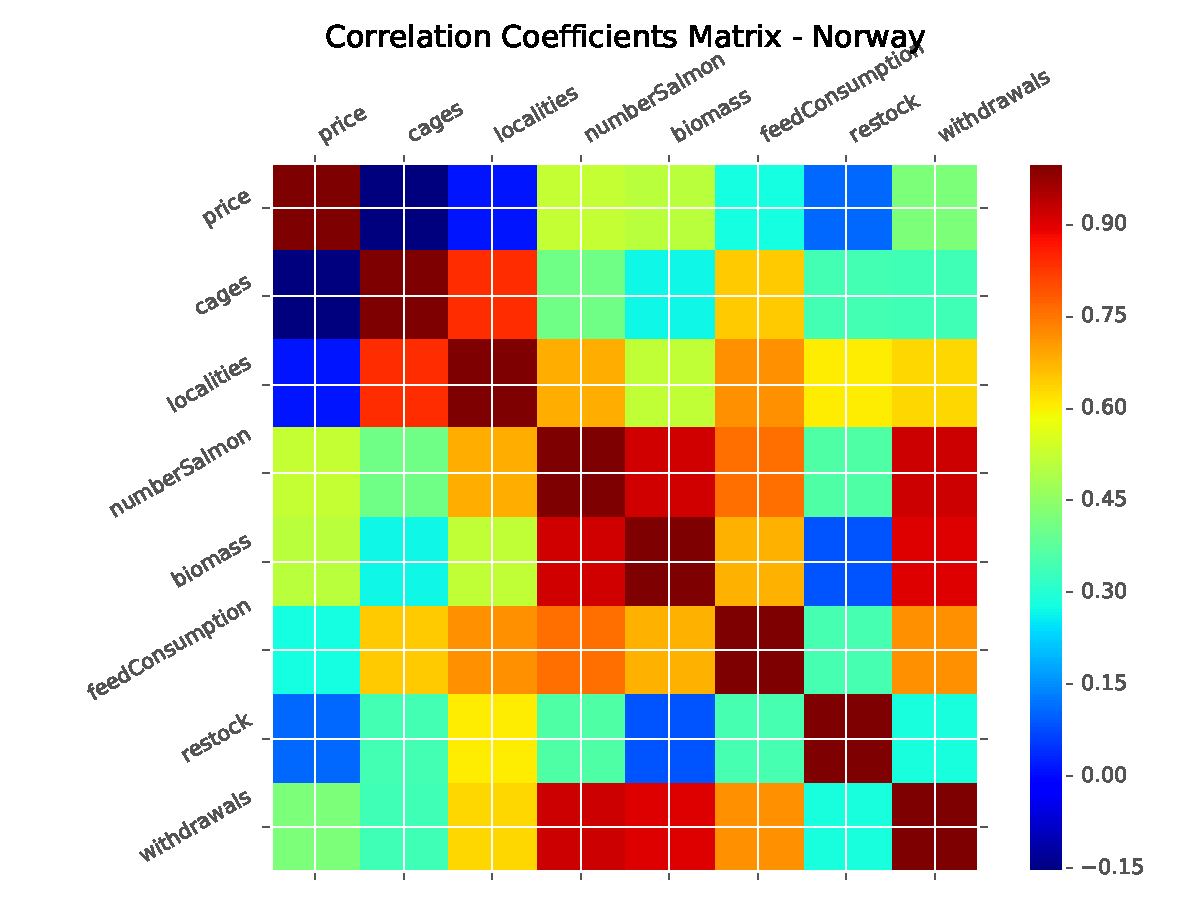
\includegraphics[width=0.85\textwidth]{Files/Total_Dataset_Matrix.pdf}
    \caption{Correlation matrix between different inputs with data.}
\end{figure}

\subsection{MIA section II: Normalized Angular Coefficients}
\textbf{Goal:}\\
Display the comparison graphic between the normalized angular coefficient of each input trend line.

\textbf{Requirements:}\\
To let the MIA system works in a proper way, is necessary that the current dataset has been already analyzed from the SIA system.

\textbf{Implementation:}\\
Also to reach this goal have been used the two libraries "pandas" and "pyplot". The first one allows us to read the values that the library "pyplot" will display, in this case in a histogram.
\begin{lstlisting}
pandas.read_csv()
pyplot.barh()
\end{lstlisting}

It's possible to check out the full ccommented code in the appendice: [\ref{MIA_section_II}]

\textbf{Results:} \\
This part of the MIA implementation allows to display a graphic that compare the normalized angular coefficients for each single input that have been already calculated and reported in a document. The result graphic look like:

\begin{figure}[H]
	\centering
    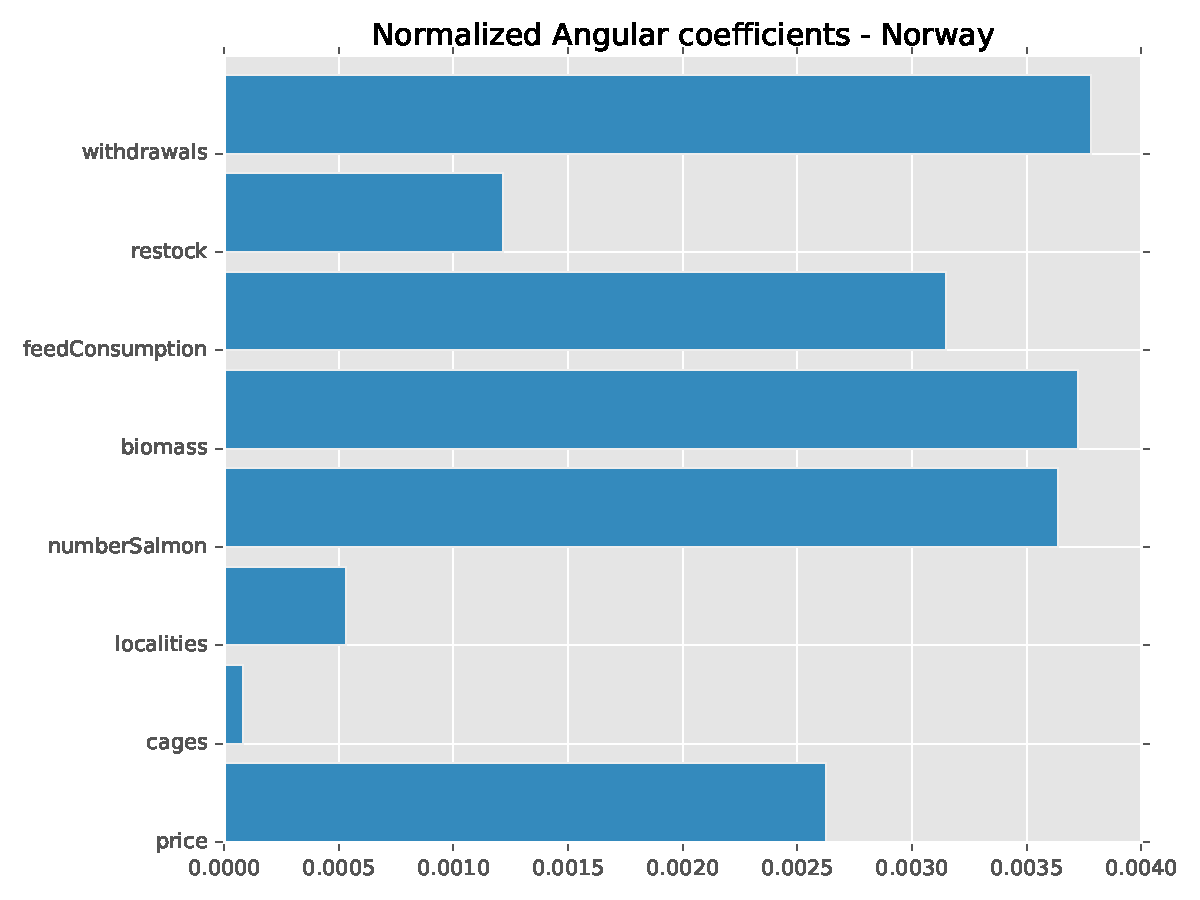
\includegraphics[width=0.90\textwidth]{Files/Norm_Ang_Coeffs.pdf}
    \caption{Normalized angular coefficients of each input's trendline.}
\end{figure}


\newpage

\section{Data Displaying on a map}
\label{Map_displaying}
\textbf{Goal:}\\
The main goal of this phase is to find a way to visualize some data values on a map graphic using Python. In this particular case the map graphic has to represents the Norway territory and its every single county.


\textbf{Requirements:}\\
This displaying system was implemented just for displaying data about Norway, that means it's not reusable for other input datasets.

During this work has been created a specific dataset for test the system works. It contains the average value of a specific input about a single county on the whole available period. The following table shows some examples about the dataset structure: for each county has been calculated the average value from 2007 to 2014 of different parameters.\\

\makebox[\textwidth][c]{
\resizebox{1.2\textwidth}{!}{
    \begin{tabular}{ | l | l | l | l | l | l |}
            \hline
\textbf{county}						&	\textbf{averageSeaTemp}	&	\textbf{cages}				& \textbf{localities}			& \textbf{...}	&  \textbf{feedConsumption/biomass}
	\\ \hline
Finnmark					&	5.2128134819	&	257.2395833333		&	33.8333333333		& ...	& 0.1611964666	\\ \hline
Troms						&	6.2185416667	&	393.3958333333		&	52.1666666667		& ...	&	0.1831404686	\\ \hline
Nordland 					&	6.8333444959	&	804.5104166667		&	109.0208333333		& ...	&	0.1849358645	\\ \hline
Nord-Trondelag				&	7.322600258		&	231.6875			&	30.3645833333		& ...	&	0.1852350478	\\ \hline
Sor-Trondelag				&	7.5381376237	&	306.9479166667		&	51.3645833333		& ...	&	0.1862036956	\\ \hline
More\_og\_Romsdal				&	8.0087820154	&	347.3229166667		&	59.5729166667		& ...	&	0.1831662176	\\ \hline
Sogn\_og\_Fjordane			&	8.1081250683	&	318.9583333333		&	52.5				& ...	&	0.1863151035	\\ \hline
Hordaland					&	7.8033025443	&	738.8854166667		&	131.1770833333		& ...	&	0.1925203347	\\ \hline
Rogaland\_og\_Agder 			&	7.1951075619	&	338.53125			&	53.0416666667		& ...	&	0.1840209916	\\ \hline
    \end{tabular}}}\\
    

\textbf{Implementation:}\\
The library "cartopy", that basically provdes cartographic tools for Python. More specifically, the most useful classes used during this part of the work have been "cartopy.io.shapereader", that allows to read the file extension ".shp"\footnote{See the definition of Shapefile: \\ \url{https://en.wikipedia.org/wiki/Shapefile}}, and "cartopy.crs", that allows to use several projections with the same interface.\\
It's possible to check out more details about the needed libraries in the appendice: [\ref{Map_libraries}]
\begin{lstlisting}
import cartopy.crs as ccrs
import cartopy.io.shapereader as shpreader
shpreader.Reader(filename).geometries())
\end{lstlisting}

\newpage

Then the input shapely geometries were displayed  to the axes using the "matplotlib".
\begin{lstlisting}
plt.figure()
ax = plt.axes()
axes.add_geometries
\end{lstlisting}

Once displayed the geometries on the map, is possible to set their colors based on some input values with the library "matplotlib".
\begin{lstlisting}
plt.get_cmap
matplotlib.colors.Normalize
\end{lstlisting}

It's possible to check out the full ccommented code in the appendice: [\ref{Map_System}]

\textbf{Results:} \\
During this implementation was implemented a cartographic representation of some parameters about each single county involved in the Norwegian aquaculture business, but is possible to use the reported library to implement a system about an another territory or an another country.
\begin{figure}[H]
    	\makebox[\textwidth][c]{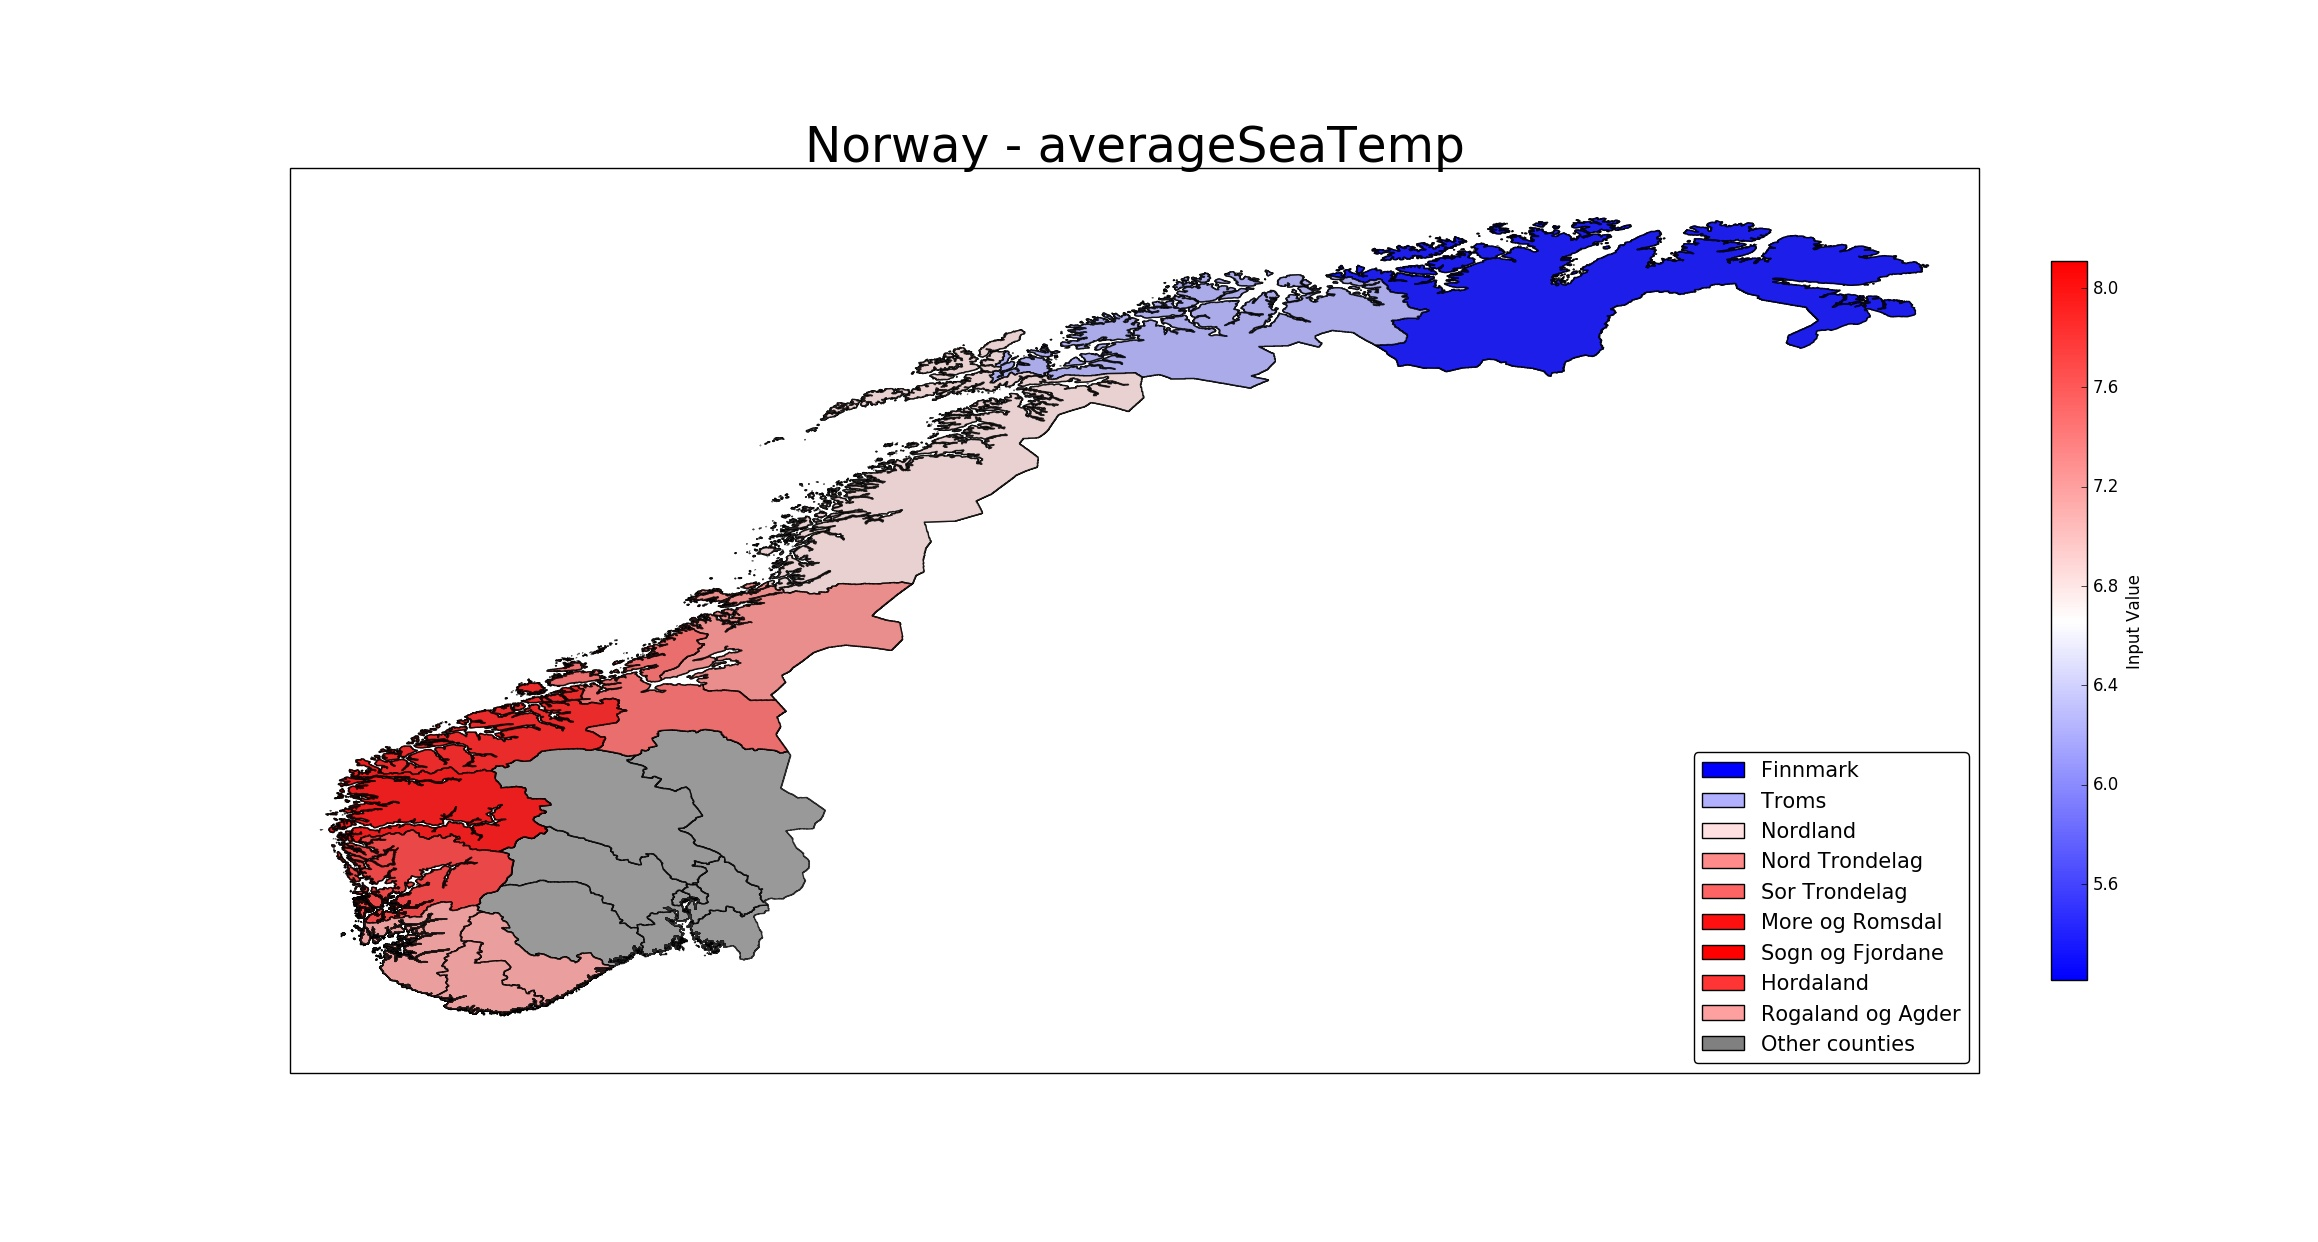
\includegraphics[trim={0cm 2cm 0 3cm},clip, width=1.4\textwidth]{Files/norway_averageSeaTemp.jpeg}}
    \caption{Monthly Average Sea Temperature from 2007 to 2014 in Norway.}
\end{figure}


\chapter{Prediction System}

Some basic and general goals were defined before starting this phase, with the idea of "doing as much as possible". \\
The main purpose was the one of, after the previous analysis, predict some values and evaluate the quality of the results.
This prediction system was not defined with some specific requirements, so the first main problem was to find a reliable, accurated and user-friendly way to predict and display prediction of values.

Since the current dataset can be considered like a time series, in this phase we will develop the data prediction system using an ARIMA machine implemented in python.

The ARIMA machine can be configured with several configurations, it allows you to have more accurated results; so the first thing was to find the right configuration of the ARIMA machine of each single input which we are interested to forecast.

During this phase of the work have been implemented 3 different subsystems for different purposes:
\begin{enumerate}
\item Evaluating System
\item Prediction System
\end{enumerate}

\newpage
\section{Evaluating System}
\textbf{Goal:}\\ 
Used for evaluate different configurations of ARIMA machine. \\ It tests 112 different configurations for the current input that we would like to forecast and report the results with each MAPE (Mean Average Percentage Error) values.

\textbf{Requirements:}\\
There are not any kind of needed requirements. It's possible to use this system on dataset of arbitrary length.

\textbf{Code implementation:}\\
The most important part of the code about the Evaluating System is the following.\\
Basically the method ARIMA() allows to train a model based on historic values (history) and a specific order (p,d,q). After that it's possible to call the method forecast() through the trained model and having some predictions like result.
\begin{lstlisting}
model = ARIMA(history, order=arima_order)
model_fit = model.fit(disp=0)
yhat = model_fit.forecast()[0]
\end{lstlisting}

This system will provide 112 different ARIMA configurations results for each single input, and in particular it will display the best ARIMA configuration, that is the one with the lower MAPE.

\textbf{Results:}\\
The system will display the MAPE between real value and predicted values for each single tested ARIMA machine, in particular the configuration that gives the best result.
All these results have been reported in a document and then also displayed with a 3D graphic that allows to see the MAPE value for each different order in input.

\begin{figure}[H]
	\raggedleft
	\makebox[\textwidth][c]{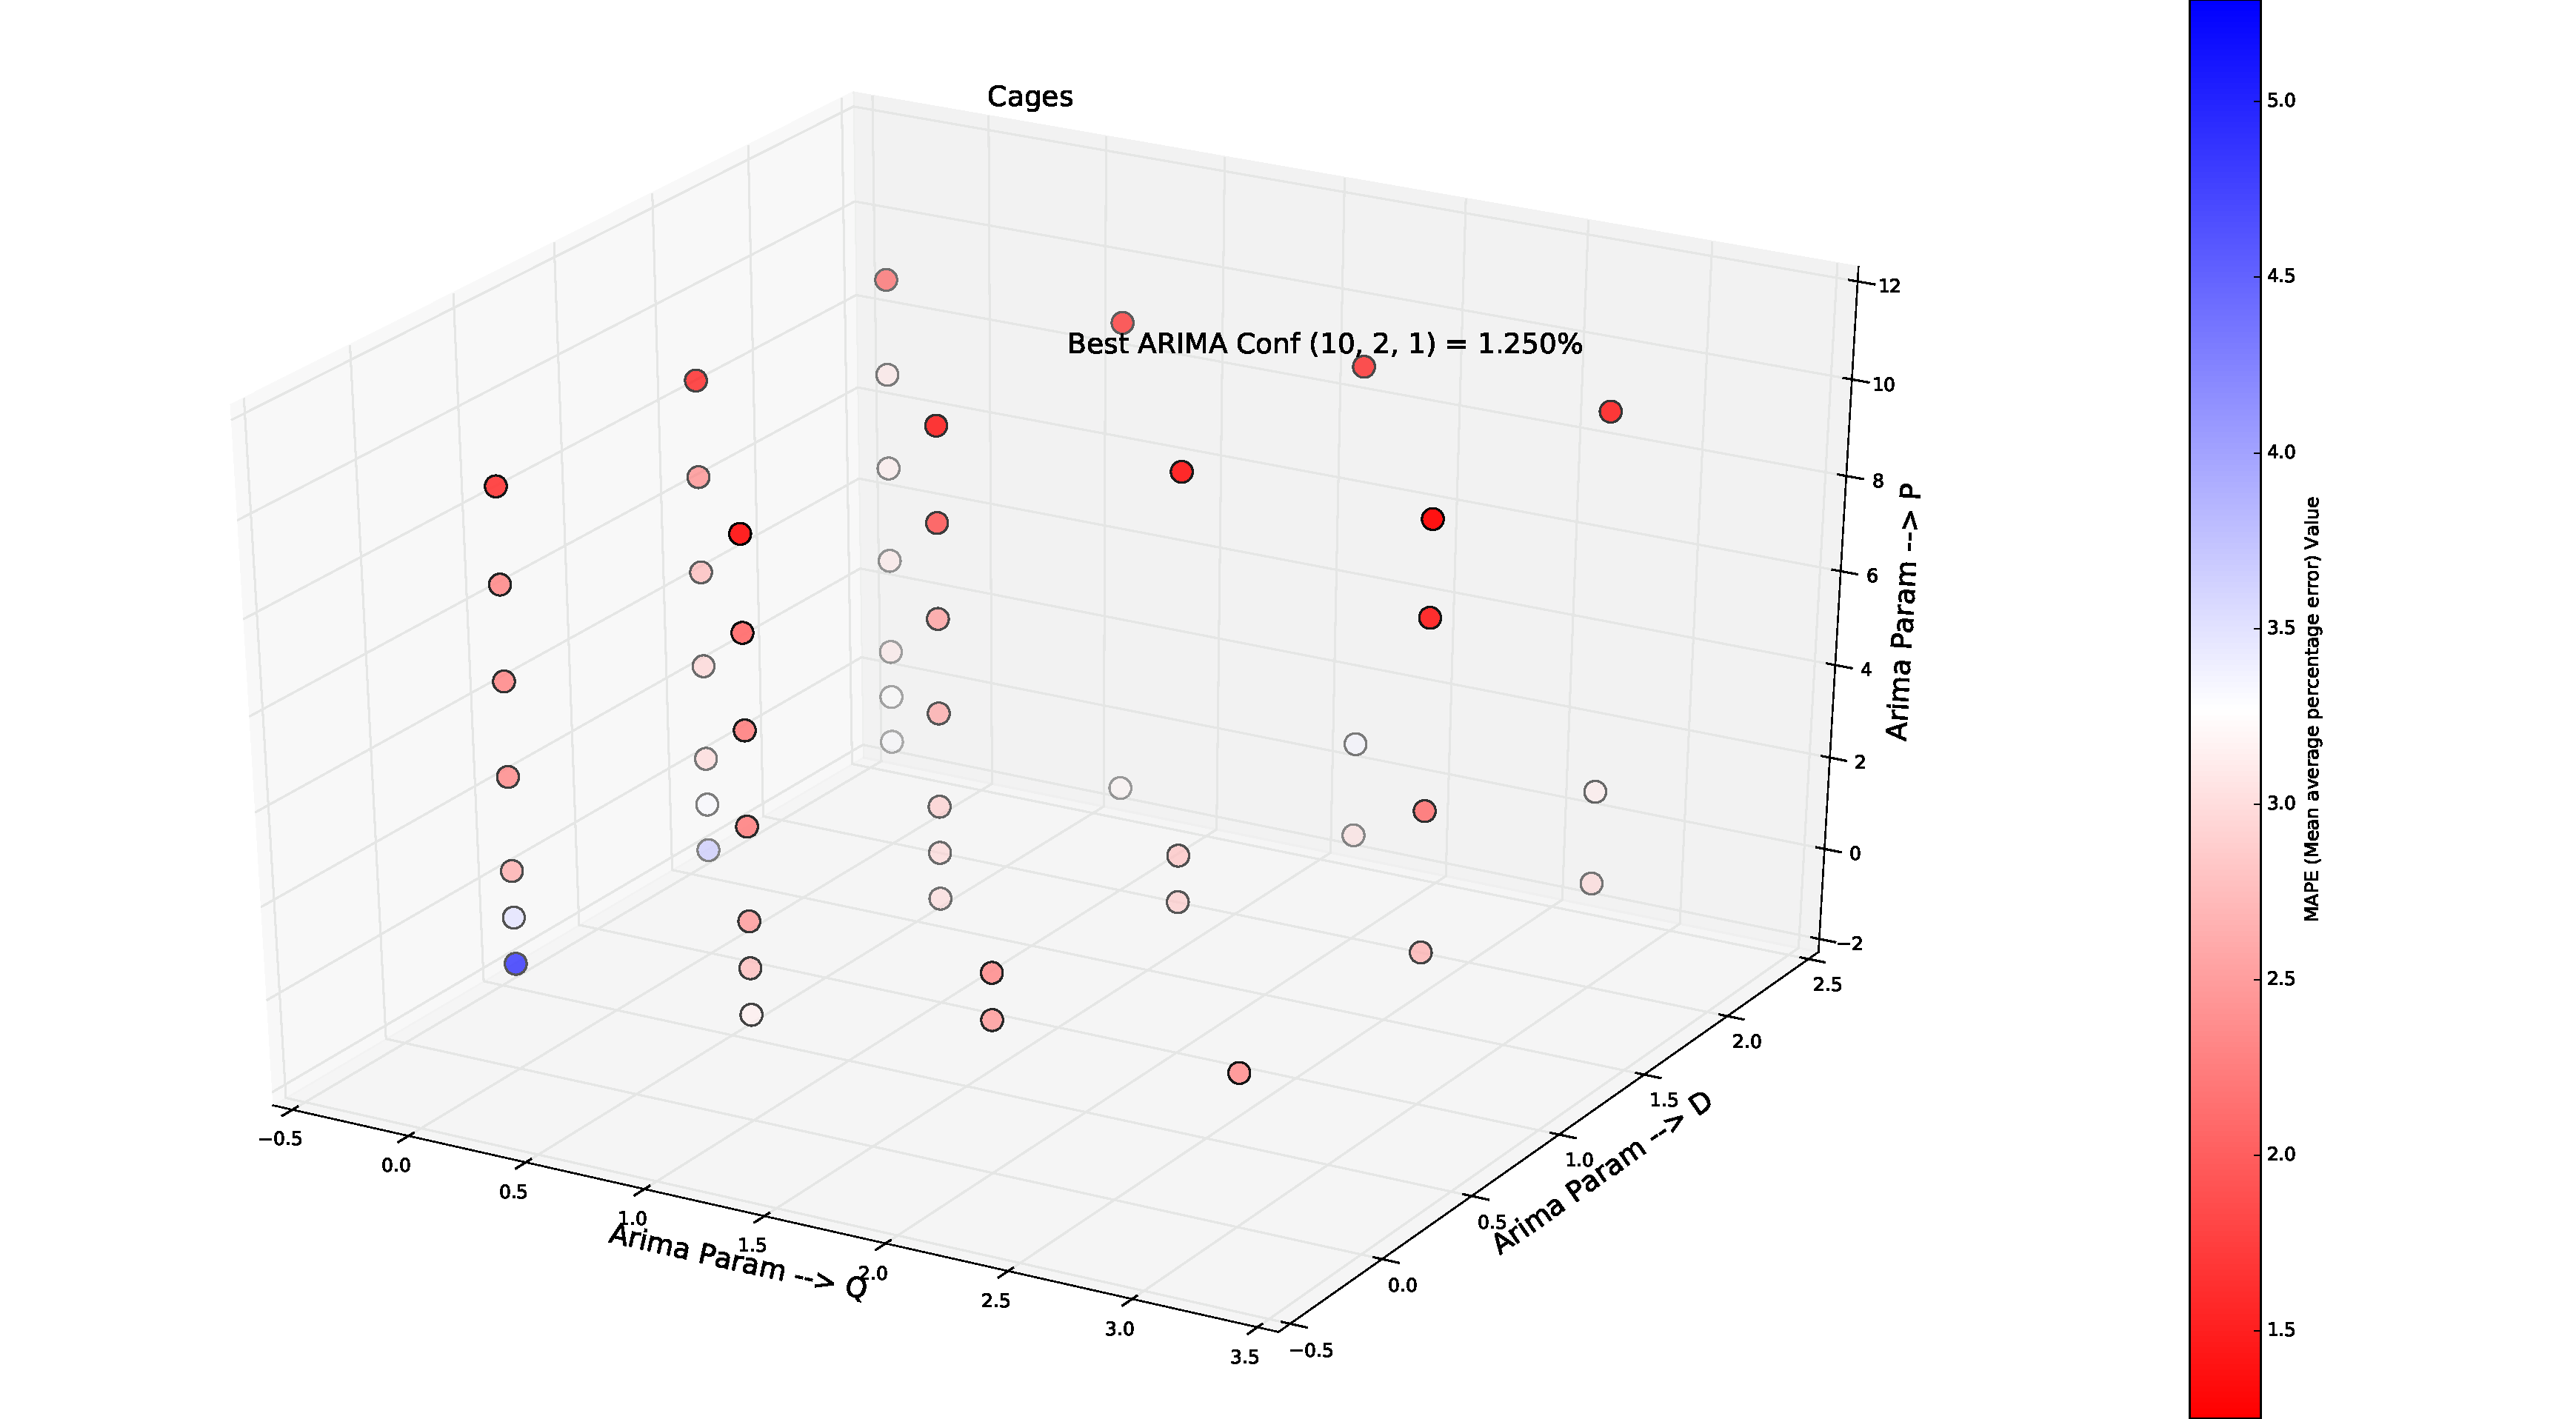
\includegraphics[width=0.6\textwidth]{Files/Cages_MAPE.pdf}}
    \caption{Graphic that displays different MAPE values for each ARIMA order.}
\end{figure}

 
 
\newpage
\section{Prediction System}
\textbf{Goal:}\\ 
This system has three main goals:
\vspace{-5mm}
\begin{itemize}
 \setlength{\itemsep}{-5pt} 
\item Testing a specific ARIMA configuration on a particular data input, and display how much accurate it is (MAPE).
\item Predict some future value with the same ARIMA configuration.
\item Display the historic data together with the testing and future predictions.
\end{itemize}

\textbf{Requirements:}\\
There are not any kind of needed requirements. It's possible to use this system on input dataset of arbitrary length.


\textbf{Code implementation:}\\
To reach the first of the goals reported above the system will divide the input dataset in two parts, train and test. It allows to train the ARIMA model with just the "train" part of the dataset, that usually is 66\% of the whole dataset, and then try to predict the rest of the dataset values, comparing in the end with the values contain in the "test" part to have a general idea about the accuracy.

The method ARIMA() allows to train a model based on historic values (history) and a specific order (p,d,q). After that it's possible to call the method forecast() through the trained model and having some predictions like result.

\begin{lstlisting}
model = ARIMA(history, order=arima_order)
model_fit = model.fit(disp=0)
yhat = model_fit.forecast()[0]
\end{lstlisting}

Then the system will also predict a number of future values choosen by the system user.
\begin{lstlisting}
model = ARIMA(dataset, order=order)
model_fit = model.fit(disp=0)
forecast = model_fit.forecast(int(sys.argv[3]))[0]
\end{lstlisting}

The final step is to display the historic data together with the test prediction and the future prediction on the same graphic. 
\begin{lstlisting}
# Plot current input's historic values 
series.plot(color="blue", linewidth=1.5, label="Series: "+sys.argv[1])

# Plot current input's test prediction
predHistoric.plot(color="red", linewidth=1.5, label="Prediction test:")

# Plot current input's future prediction
predFuture.plot(color="green", linewidth=1.5, label="Future Prediction:")

\end{lstlisting}

\textbf{Results:}\\
This system will automatically generate two documents that contain:
\vspace{-5mm}
\begin{itemize}
 \setlength{\itemsep}{-5pt} 
\item Test predictions values
\item Future predictions values
\end{itemize}

And then it provides also the possibility to visualize the historic, test and future predictions values on the same graphic, that looks like the following example:

\begin{figure}[H]
	\centering
    \makebox[\textwidth][c]{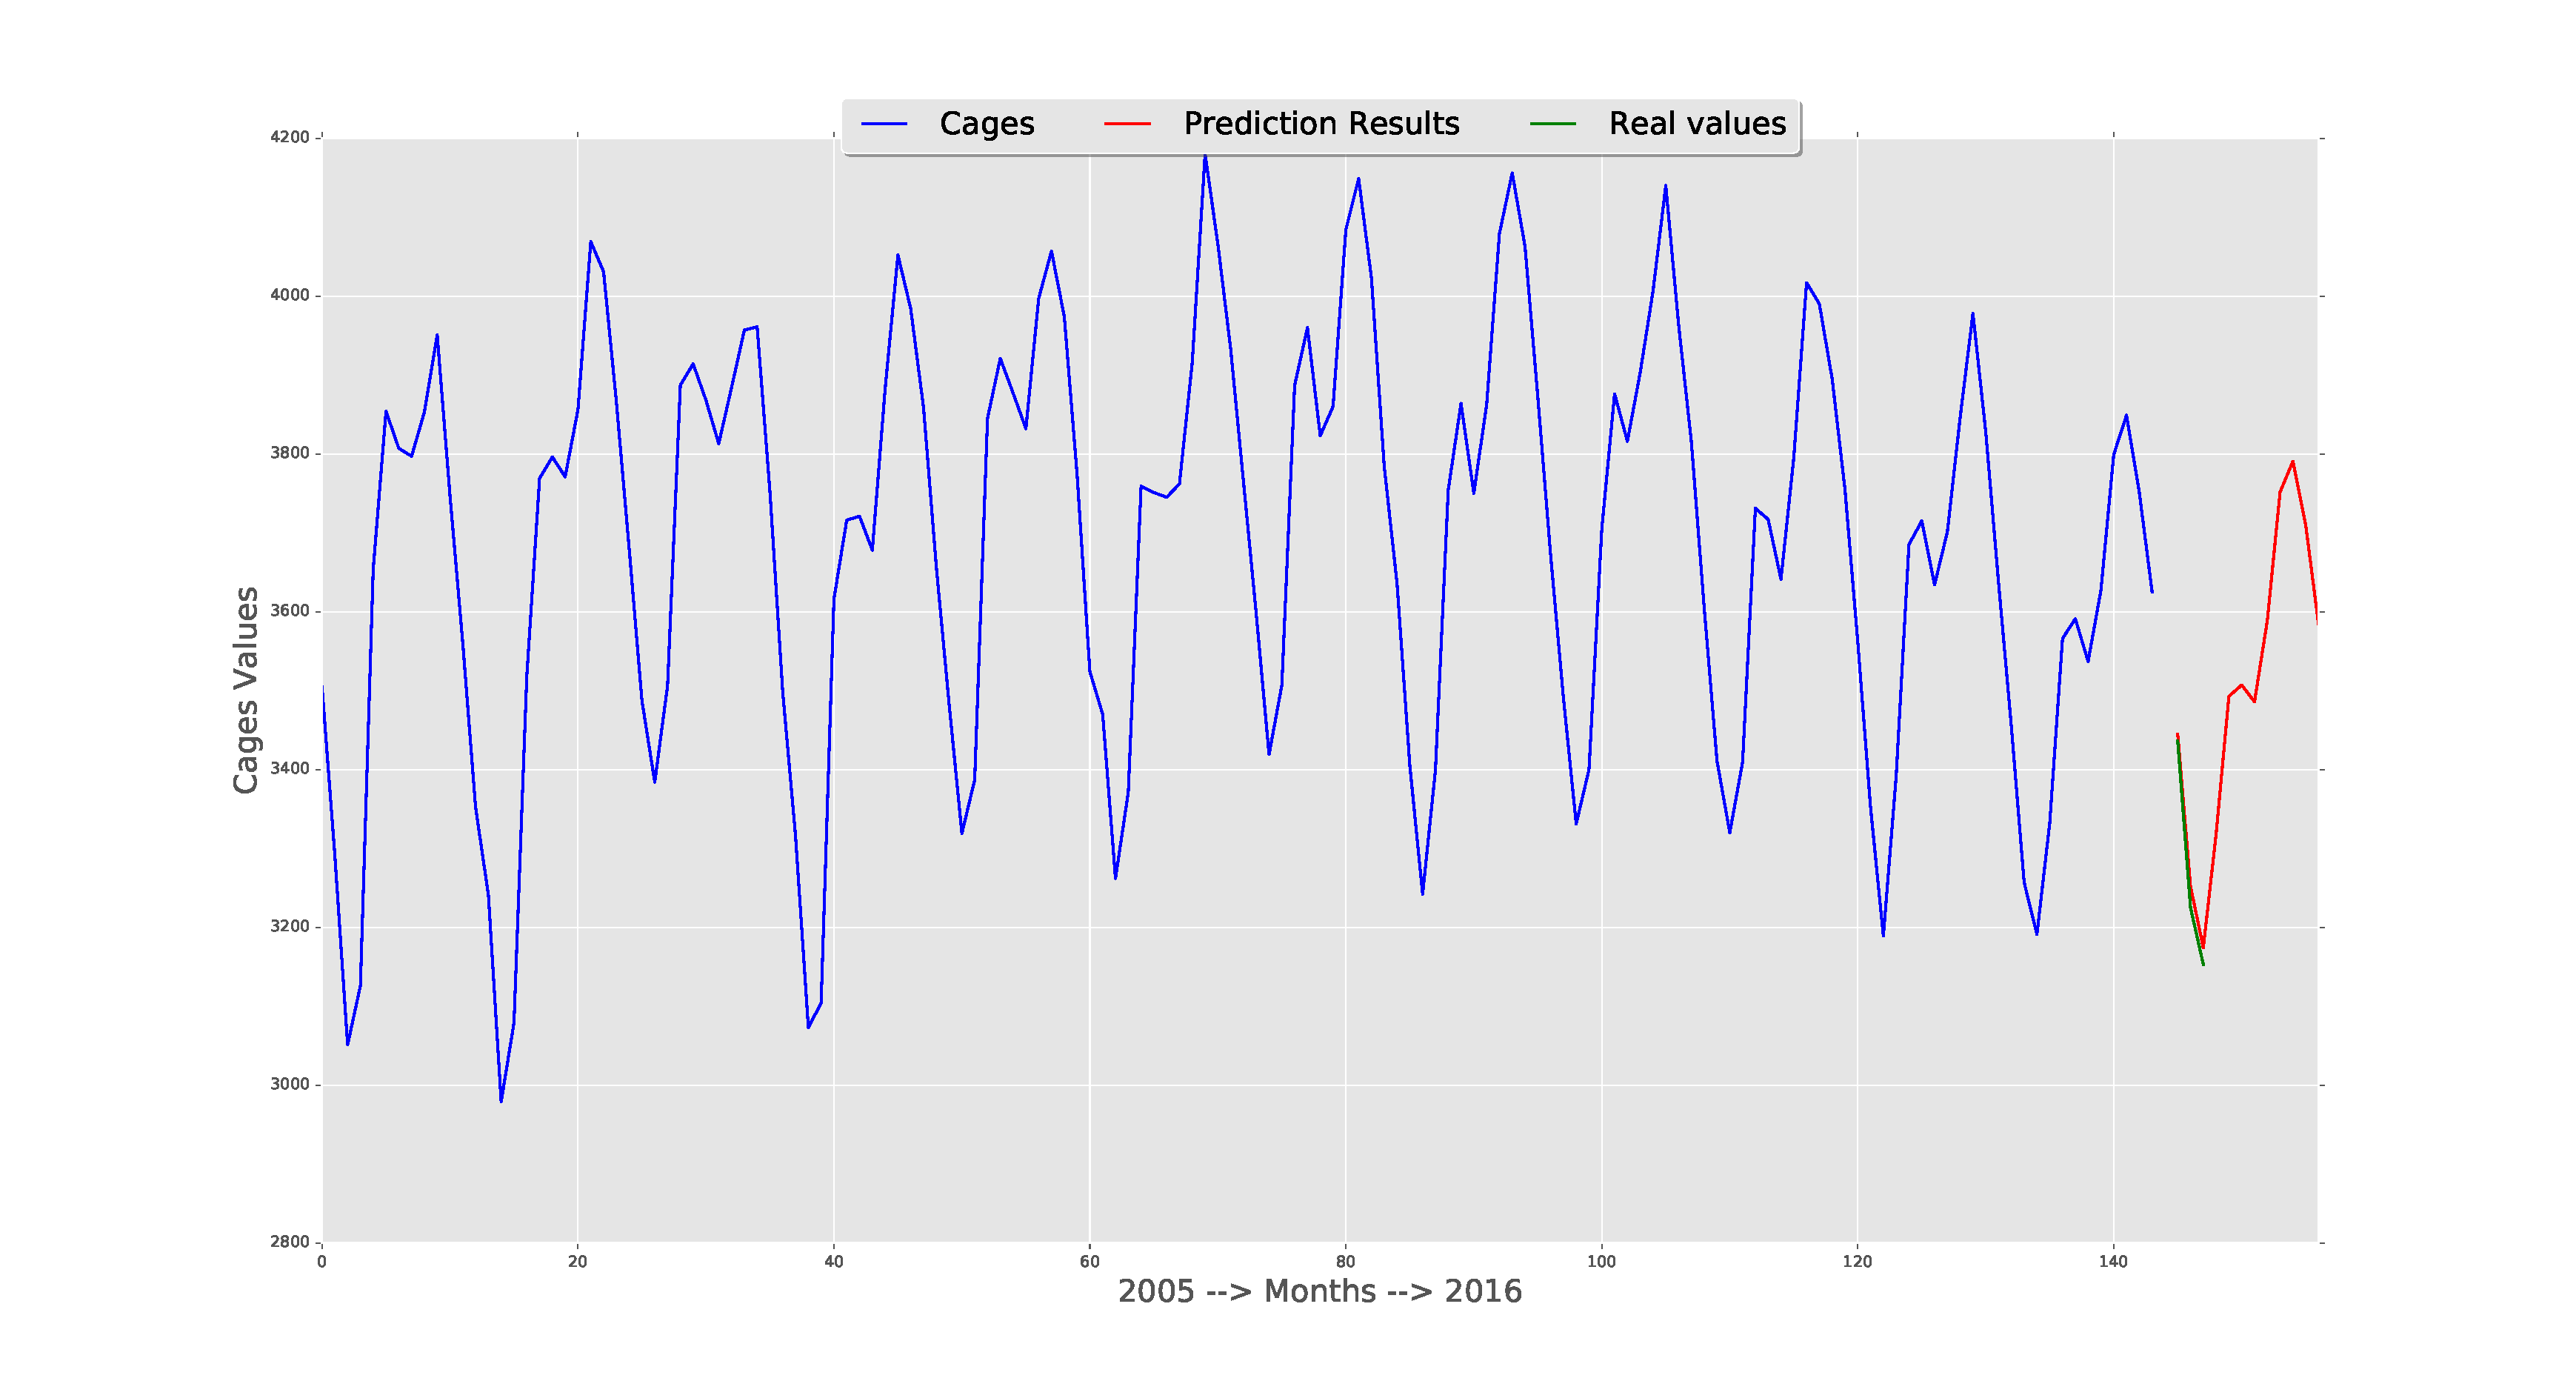
\includegraphics[width=1.5\textwidth]{Files/Cages_Predictions.pdf}}
    \caption{Graphic that display historic, future and predicted values of a input.}
\end{figure}


\newpage





\part{Discussion, Evaluations and Conclusions}
%
\chap{Results}

The main result of this work is the implemented "Python Analyzer System" itself. It actually provides an automatic way to make an initial analysis and display the results of any input dataset.

Further more has been provided an initial Python implementation of:
\begin{itemize}
\item Future Prediction System
\item Country Map Displaying System
\end{itemize}
\newpage

\begin{figure}[H]
	\centering
    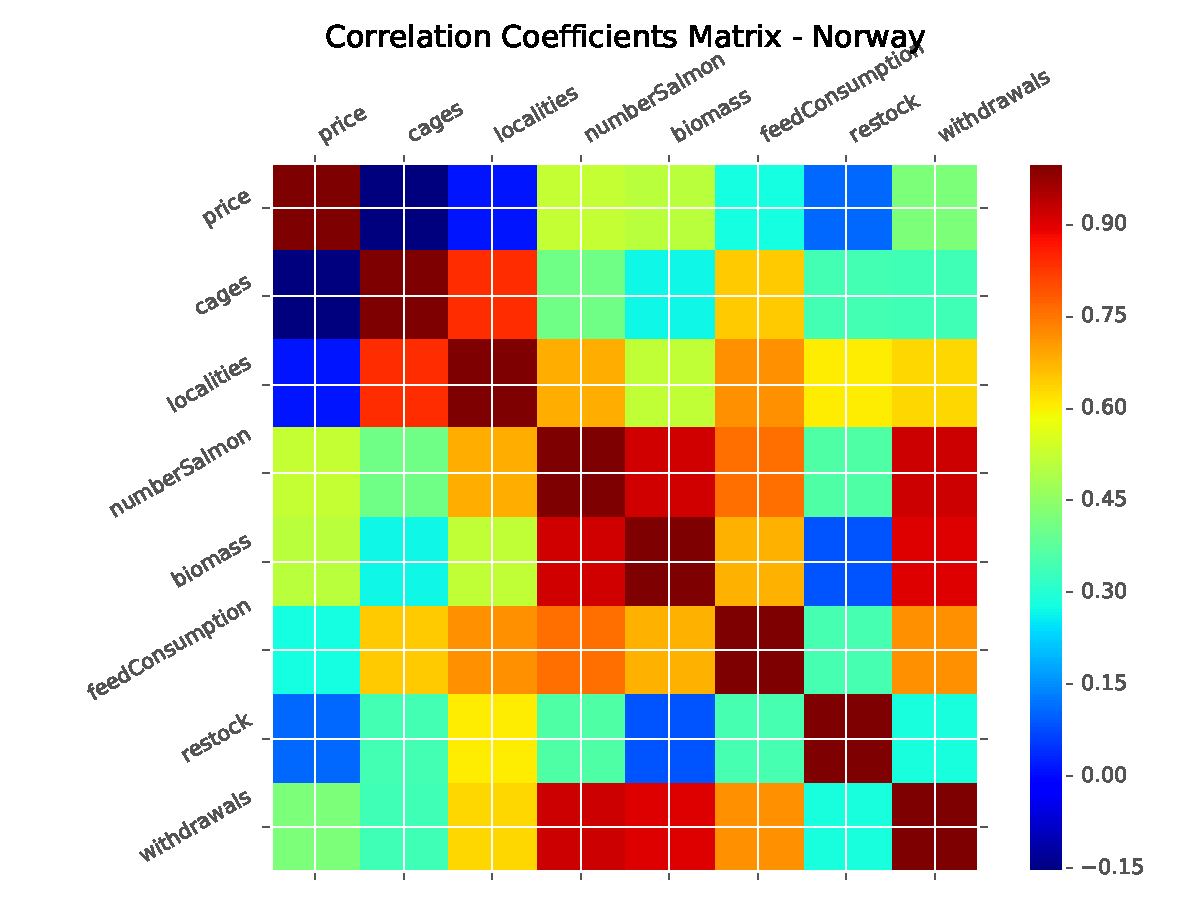
\includegraphics[width=1\textwidth]{Files/Total_Dataset_Matrix.pdf}
    \caption{Correlation matrix between different inputs with data from 2005 to 2016.}
\end{figure}

\begin{table}[ht] 
\makebox[\textwidth][c] {
\resizebox{1.2\textwidth}{!}{\begin{tabular}{ | l | l | l | l | l | l | l | l | l |}
        \hline
INPUTS	& Price 		& Cages 			& Localities		& numberSalmon 		& biomass 		& feedConsumption 		& restock 		& withdrawals 				\\ \hline
Price			& 1			& -0.16		& 0.02 		& 0.52		& 0.51		& 0.28		& 0.11 		& 0.43		\\ \hline
Cages			& -0.16		& 1			& 0.84		& 0.41		& 0.27		& 0.64		& 0.34		& 0.34		\\ \hline
Localities		& 0.02		& 0.84		& 1			& 0.68		& 0.52		& 0.72		& 0.6		& 0.63		\\ \hline
numberSalmon	& 0.52		& 0.41		& 0.68		& 1 		& 0.92		& 0.76		& 0.36		& 0.92		\\ \hline
biomass			& 0.51		& 0.27		& 0.52		& 0.92		& 1			& 0.68		& 0.09		& 0.91		\\ \hline
feedConsumption	& 0.28		& 0.64		& 0.72		& 0.76		& 0.68		& 1			& 0.35		& 0.72		\\ \hline
restock			& 0.11		& 0.34		& 0.6		& 0.36		& 0.09		& 0.35		& 1 		& 0.28		\\ \hline
withdrawals		& 0.43		& 0.34		& 0.63		& 0.92		& 0.91		& 0.72		& 0.28		& 1			\\ \hline
    \end{tabular}}}
    \caption{Dataset inputs correlation coefficients value.}
    \label{table: trendline} 
\end{table}

\newpage

\begin{figure}[H]
	\centering
    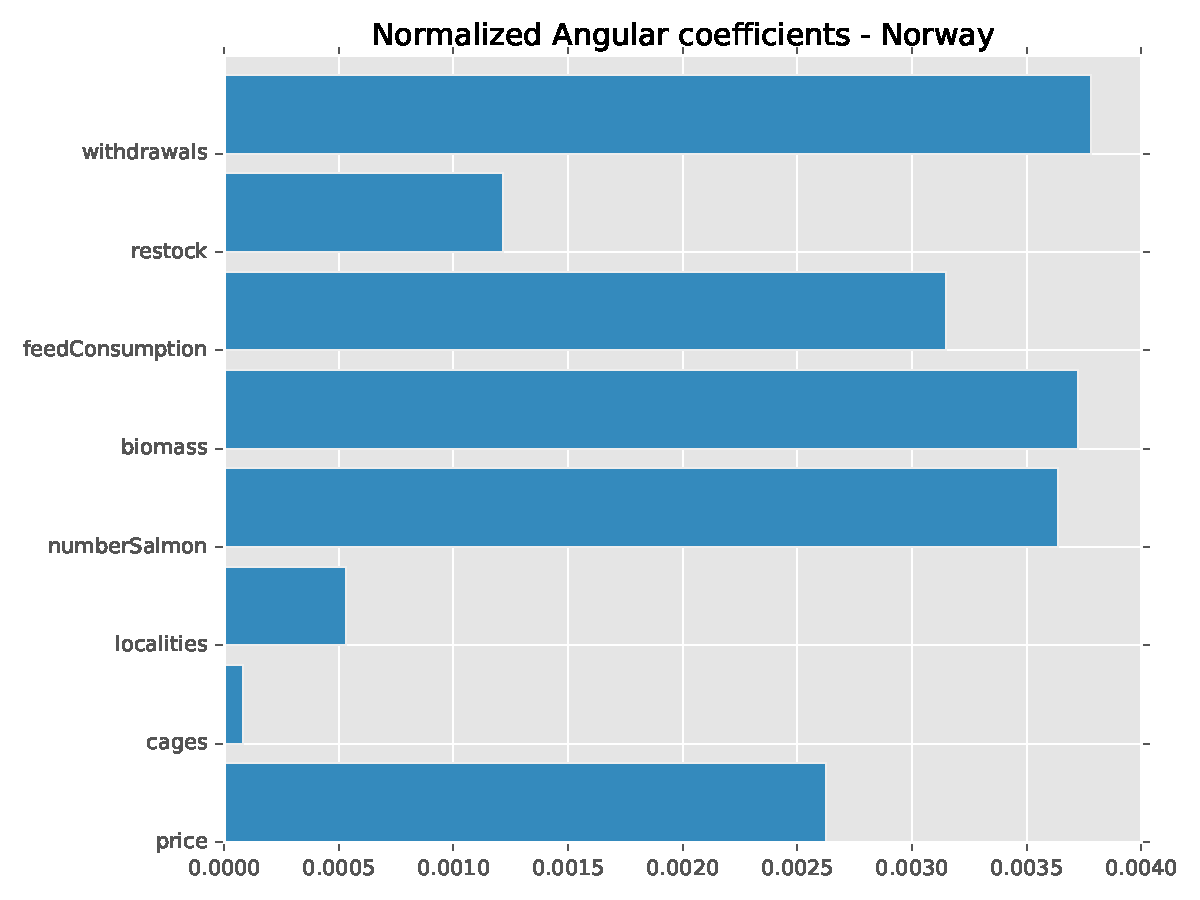
\includegraphics[width=1\textwidth]{Files/Norm_Ang_Coeffs.pdf}
    \caption{Normalized angular coefficients of each input's trendline.}
\end{figure}

\begin{table}[ht] 
	\centering
    \begin{tabular}{ | l | l | l | p{5cm} |}
        \hline
        Input 								& Equation 							& Coeff			\\ \hline
          	Salmon\_withdrawals 			& y=464.755139x+(46295.729945) 		& 464.755139 	\\ \hline
          	Salmon\_biomass\_end\_month 	& y=2832.712270x+(354138.727889) 	& 2832.71227 	\\ \hline
          	Salmon\_number\_end\_month 		& y=1543.298421x+(205325.455772)	& 1543.298421 	\\ \hline
          	Salmon\_consumption\_of\_feed 	& y=620.070855x+(58330.012273) 		& 620.070855	\\ \hline
           	Salmon\_price 			& y=0.178175x+(22.643654)			& 0.1781753878 		\\ \hline
          	Salmon\_restock 				& y=89.230600x+(13390.363406)		& 89.2306 		\\ \hline
 			Localities 						& y=0.343533x+(539.979023) 			& 0.343533		\\ \hline
  			Cages 							& y=0.342834x+(3665.904023) 		& 0.342834 		\\ \hline
    \end{tabular} 
    \caption{Dataset inputs trendline equation}
    \label{table: trendline} 
\end{table}
\begin{table}[ht] 
	\centering
    \begin{tabular}{ | l | l | l | p{5cm} |}
        \hline
        Input 							& Normalized equation 	& Norm Ang Coeffs	\\ \hline
          	Salmon\_withdrawals 		& y=0.003782x+(0.376694)& 0.003782			\\ \hline
          	Salmon\_biomass\_end\_month & y=0.003724x+(0.465599)& 0.003724			\\ \hline
          	Salmon\_number\_end\_month 	& y=0.003639x+(0.484184)& 0.003639			\\ \hline
          	Salmon\_consumption\_of\_feed & y=0.003147x+(0.296085)& 0.003147		\\ \hline
           	Salmon\_price 		& y=0.002625x+(0.333633)
& 0.002625			\\ \hline
          	Salmon\_restock 			& y=0.001217x+(0.182583)& 0.001217			\\ \hline
 			Localities 					& y=0.000531x+(0.834589)& 0.000531			\\ \hline
  			Cages 						& y=0.000082x+(0.877011)& 0.000082			\\ \hline
    \end{tabular} 
    \caption{Dataset inputs normalized trendline equation}
    \label{table: norm_trendline} 
\end{table}

\newpage

\begin{figure}[H]
    \makebox[\textwidth][c]{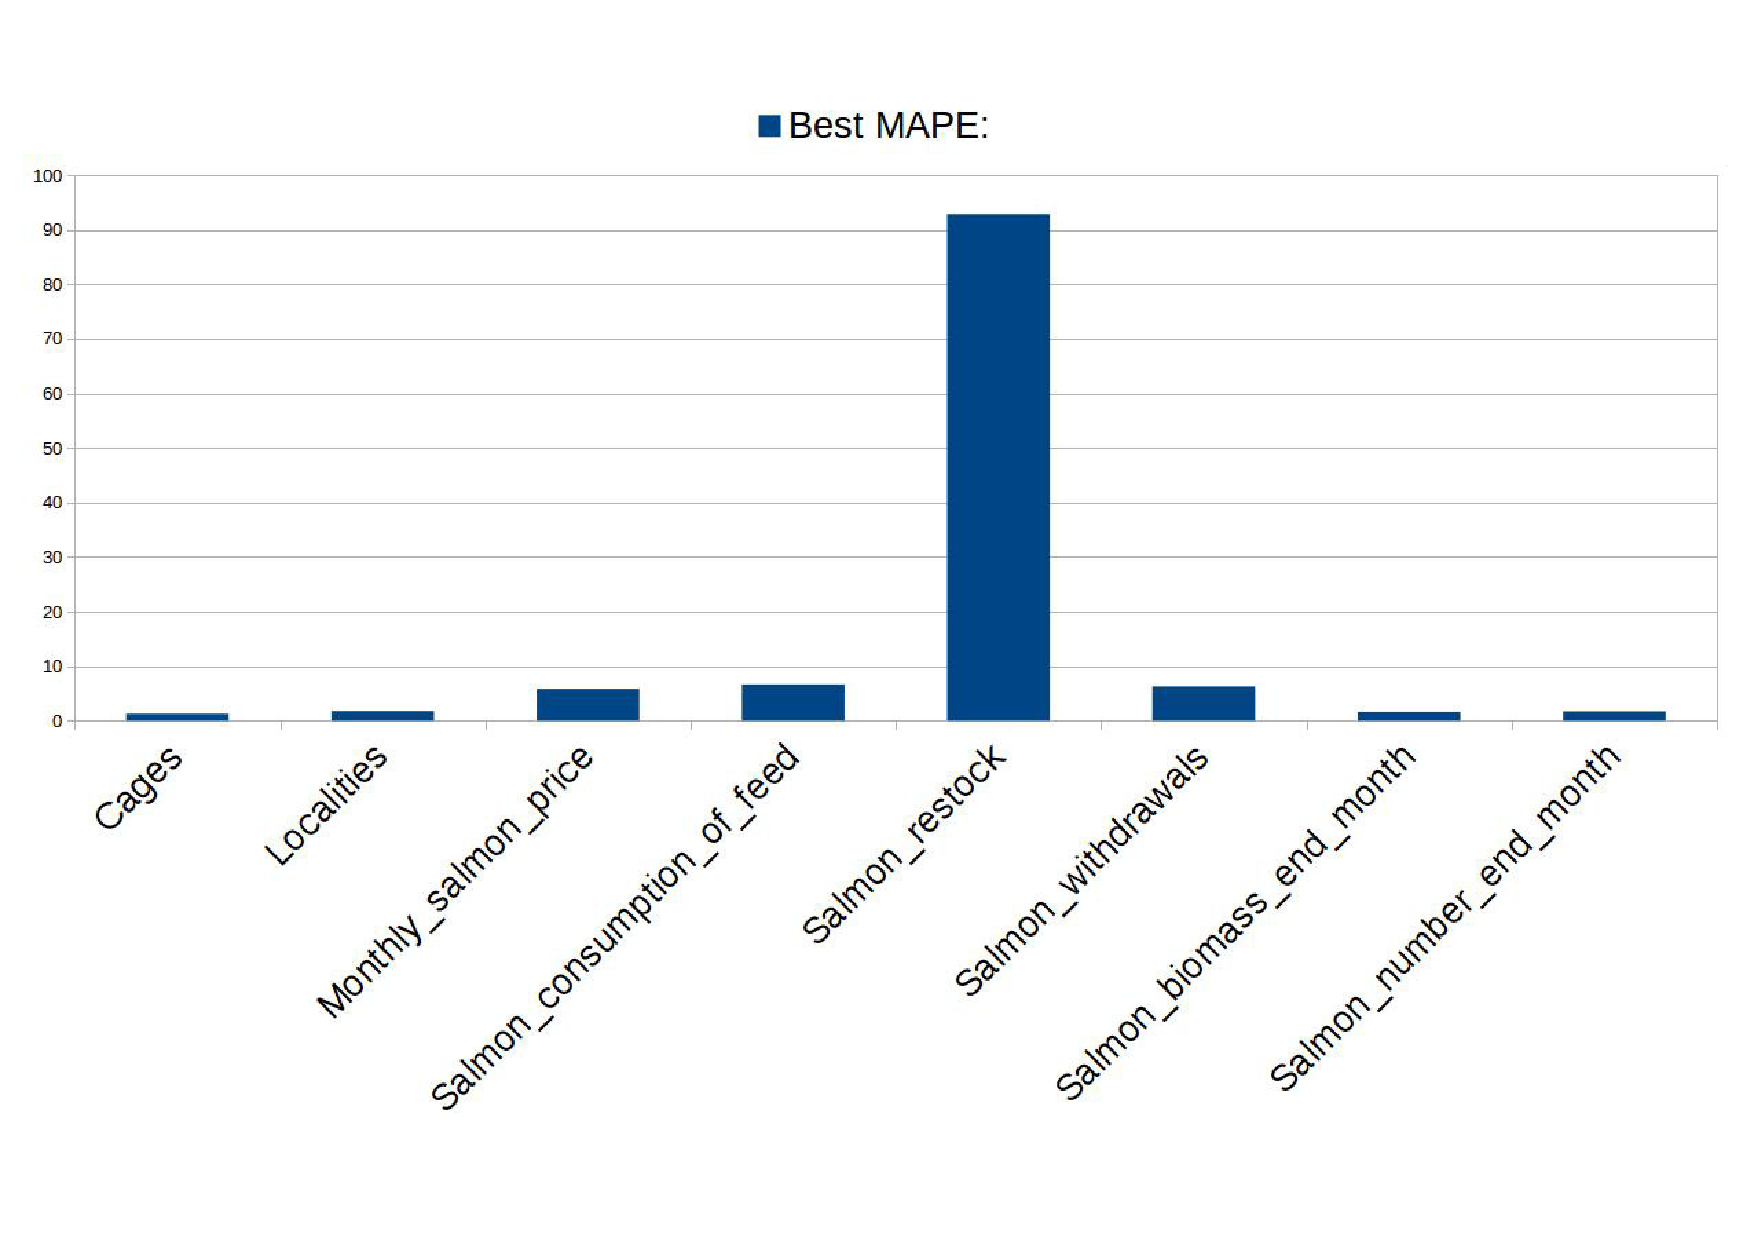
\includegraphics[width=1.2\textwidth]{Files/Best_MAPE.pdf}}
    \caption{Lower MAPE with best ARIMA Configuration for each tested input.}
\end{figure}

\begin{table}[ht] 
	\centering
    \begin{tabular}{ | l | l | l |}
            \hline
Input							&	ARIMA Conf	&	MAPE	\\ \hline
Cages							&	(10,2,1)	&	1.251\%	\\ \hline
Localities						&	(10,0,1)	&	1.779\%	\\ \hline
Salmon\_price 					&	(0,1,1)		&	6.686\%	\\ \hline
Salmon\_consumption\_of\_feed	&	(6,1,0)		&	6.659\%	\\ \hline
Salmon\_restock 				&	(10,0,1)	&	96.006\%	\\ \hline
Salmon\_withdrawals 			&	(10,0,1)	&	6.277\%	\\ \hline
Salmon\_biomass\_end\_month		&	(8,1,0)		&	1.601\%	\\ \hline
Salmon\_number\_end\_month 		&	(10,2,0)	&	1.723\%	\\ \hline
    \end{tabular}  
    \caption{Dataset inputs normalized trendline equation}
    \label{table: Best ARIMA configurations with relative MAPE result in the Evaluation Test} 
\end{table}

\newpage

\makebox[\textwidth][c]{
\resizebox{1.3\textwidth}{!}{
\begin{tabular}{|c|c|c|c|c|c|c|c|c|c|c|c|c|c|}
\hline
\multirow{3}{*}{Months} & \multicolumn{3}{c|}{Cages} & \multicolumn{3}{c|}{Localities} & \multicolumn{3}{c|}{Salmon Biomass} & \multicolumn{3}{c|}{Salmon Number}\\
\cline{2-13}
 & Real & Pred & Error & Real & Pred & Error & Real & Pred & Error & Real & Pred & Error \\
\hline
 January 2017 & 3436 & 3444.87 & 0.26\% & 539.000 & 543.41 & 0.82\% & 738902 & 732841.36 & 0.82\% & 369274 & 366826.189 & 0.66\%\\
\hline
 February 2017 & 3225 & 3251.915 & 0.83\% & 523.000 & 529.05 & 1.16\% & 712981 & 709931.42 & 0.43\% & 347824 & 352905.30 & 1.46\% \\
 \hline
 March 2017 & 3153 & 3164.190 & 0.67\% & 529.000 & 534.29 & 1.00\% & 667749 & 679405.11 & 1.75\% & 343636 & 349747.77 & 1.78\%\\
 \hline
 April 2017 & & 3317.814 & & & 549.14 & & & 657418.41 & & & 369616.83 &  \\
 \hline
 May 2017 & & 3492.701 & & & 550.64 & & & 646850.14 & & & 387244.43 &  \\
 \hline
 June 2017 & & 3507.062 & & & 545.66 & & & 653574.18 & & & 387630.48 & \\
 \hline
 July 2017 & & 3485.804 & & & 560.58 & & & 678469.77 & & & 384314.00 &  \\
 \hline
 August 2017 & & 3588.373 & & & 584.55 & & & 707646.99 & & & 394062.43 & \\
 \hline
 September 2017 & & 3751.633 & & & 596.32 & & & 734628.28 & & & 411164.01 & \\
 \hline
 October 2017 & & 3790.521 & & & 589.11 & & & 757679.66 & & & 411094.09 & \\
 \hline
 November 2017 & & 3710.033 & & & 576.75 & & & 770838.51 & & & 396102.24 & \\
 \hline
 December 2017 & & 3584.505 & & & 563.56 & & & 771279.10 & & & 380399.93 & \\
 \hline
% etc. ...
\end{tabular}  }}


\makebox[\textwidth][c]{
\resizebox{1.3\textwidth}{!}{
\begin{tabular}{|c|c|c|c|c|c|c|c|c|c|c|c|c|c|}
\hline
\multirow{3}{*}{Months} & \multicolumn{3}{c|}{Consumption of feed} & \multicolumn{3}{c|}{Salmon restock} & \multicolumn{3}{c|}{Salmon Withdrawals} & \multicolumn{3}{c|}{Salmon price}\\
\cline{2-13}
 & Real & Pred & Error & Real & Pred & Error & Real & Pred & Error & Real & Pred & Error \\
\hline
 January 2017 & 109341 & 98174.28 & 10.21\% & 4415 & 4734.43 & 7.23\% & 87609 & 90488.98 & 3.29\% & & &\\
\hline
 February 2017 & 88704 & 77998.20 & 12.07\% & 991 & 6904.51 & 596.72\% & 3.29\% & 101295.55 & 11.00\% & & &\\
 \hline
 March 2017 & 87033 & 74726.18 & 14.14\% & 13594 & 15427.63 & 13.49\% & 109498 & 101724.09 & 7.10\% & & &\\
 \hline
 April 2017 & & 88768.11 & & & 39781.36 & & & 95032.95 & & & &\\
 \hline
 May 2017 & & 113280.67 & & & 39438.14 & & & 92065.64 & & & &\\
 \hline
 June 2017 & & 140413.56 & & & 22562.89 & & & 88775.54 & & & &\\
 \hline
 July 2017 & & 164511.15 & & & 20449.85 & & & 92643.44 & & & &\\
 \hline
 August 2017 & & 179690.48 & & & 39487.67 & & & 104102.60 & & & &\\
 \hline
 September 2017 & & 181556.12 & & & 49991.91 & & & 110419.37 & & & &\\
 \hline
 October 2017 & & 169502.10 & & & 31449.69 & & & 107588.69 & & & &\\
 \hline
 November 2017 & & 147770.73 & & & 11698.23 & & & 102943.86 & & & &\\
 \hline
 December 2017 & & 123447.55 & & & 7957.45 & & & 99561.98 & & & &\\
 \hline
% etc. ...
\end{tabular}  }}


 % Results
\chap{Discussion and Evaluations}

The current study investigates about the possibility of testing the Data Science process using Python, trying to apply it to the Norwegian salmon farming industry, in order to gather and let be available as many useful results as possible.

\section{Evaluation and limitations of the study}
\vspace{-5mm}
This study has a number of possible limitations, mainly due to:
\vspace{-5mm}
\begin{itemize}
 \setlength{\itemsep}{-5pt}
 \item A lack of background knowledge about Data Science procedures.
 \item A lack of background knowledge about Salmon farming in Norway.
 \item Relatively short time available for this work.
 \item Limited availability of data sources.
\end{itemize}

"No one expects science to be perfect the first time and while your peers can be highly critical, no one’s work is beyond limitations. Our knowledge base is built on uncovering each piece of the puzzle, one at a time, and limitations show us where new efforts need to be made. So much like peer review, don’t think of limitations as being inherently bad, but more an opportunity for a new challenge. In the end, your limitation may be someone else’s inspiration." \cite{limitations}
  
During this work I got more and more knowledge and experience mainly about the fields reported above (Data Science procedures and Salmon farming in Norway), and it allowed to get anyway some positive and useful results that provide an answer to most of the initial objectives of this thesis. \\
In particular, this study shows that is actually possible to have a first approach to the Data Science field using Python. All the documented steps of this works allow to have a complete overview of the general Data Science process.

Furthermore, the resulting Python systems and the corresponding evidences are showing which modules and packages are provided by Python in order to analyze, display and forecast data values. The high reusability and automation levels of the implemented system allow to easily reuse it in order to apply the same analysis, displaying and forecasting on a different dataset that contains data from a different area of interest. \\
On the other side the current system is probably efficient and productive for a personal use. That's because is not provided an implemented GUI, and to customize the system's outputs you have to have some basic knowledge of Python language, that could be a sort of limitation for several people, but it could also be considered like a kind of incentive for people to get to know this powerful programming language.

The approach used for this thesis didn't provide any kind of results that can be considered as new informations about the Norwegian salmon farming field, but it provided several ideas and discussion's starting points for further works. That's because this thesis was mainly focused on the Data Science process, Python utilities and to find out observations for future researches instead of the information extraction process itself.

Even that, as reported in the Results Overview chapter, several systems, evidences and values have been calculated and reported during this work. 

In the next sections are reported evaluations and limitations about this study, and then the discussions that I considered most relevant and interesting about this work, which would also be useful for further works.

\section{Considerations about implemented Evaluation System }
The following resulting table reveals several informations. \\
The column "Evaluation MAPE" is the average MAPE of the forecasted values during the Evaluation System with the reported ARIMA order. \\ 
The column "Forecast MAPE" represents the average MAPE of the 12 values predicted in the future, already reported in the results. [\ref{table: RealPredMAPE1}] 

 \begin{table}[ht]
\makebox[1\textwidth][c]{
    \begin{tabular}{ | l | l | l | l | l |}
            \hline
\textbf{County} 	& \textbf{Parameter} & \textbf{ARIMA Order}	& \textbf{Evaluation MAPE} 	& \textbf{Forecast MAPE} 	\\ \hline
Finnmark 	& feedConsumption				& (6, 1, 0) 			& 13.771\% 	&	19.20\% 		\\ \hline	
Hordaland 	& feedConsumption				& (8, 0, 0)  			& 6.811\%	& 	17.89\%			\\ \hline				
Troms 		& feedConsumption				& (2, 0, 0)  			& 11.593\% 	&	21.05\%			\\ \hline
Nordland 	& feedConsumption				& (6, 0, 0)  			& 12.741\%	&	26.01\% 		\\ \hline
Norway0714 	& feedConsumption				& (6, 1, 0)  			& 7.296\%  	&	7.94\%			\\ \hline
    \end{tabular}}
         \caption{Comparison between Evaluation MAPE and Prediction MAPE}   
   \label{table: MAPE_Comparison} 
\end{table}        

From the values contained in the table [\ref{MAPE_Comparison}] is possible to see that the average MAPE for the forecasted future values (\textbf{Forecast MAPE}) is much higher than the one reported from the evaluation process (\textbf{Evaluation MAPE}) . \\
There is just one particular case where the Evaluation MAPE and Forecast MAPE values are really close, that is the one about the Norway dataset.

At this point, would be extremely useful to discover why the predicted future values about the dataset 'Norway0714' are much more accurate and why their average MAPE is really close to the one calculated during the evaluation procedure.

In order to understand the reason, certain analysis through the resulting evidences have been made. Below here are reported the considerations about it:
\vspace{-5mm}
\begin{itemize}
 \item Checked the annual feed consumption trend during different years for the current datasets, that is possible to check out in the reported graphics [\ref{fig: Norway_feed}]. Were not found any kind of big differences between the Norway's trend compared with the others.
 \item Checked correlation coefficients between different years of the feed consumption values for each tested dataset, but there were not any kind of significant high/low correlation levels with the years before.
 \item Tried to execute the prediction system with settings that are different by the one suggested in the Evaluation system results. Found that for some particular dataset is possible to get better predictions with a different configuration, like for example: \\
 Prediction system about "feed Consumption" in Nordland executed with the suggested configuration (6,0,0) gave a average MAPE value equal to 26.01\% for the predicted values. If the Prediction system is tested on the same input but fitting the ARIMA model with the order (6,1,0) the average MAPE value decrease to 16.82\% for the predicted values. \\
 It's possible to clearly see this different watching at the graphics reported in the following page: [\ref{fig: Nordland_ARIMAevaluation}] and [\ref{fig: Nordland_ARIMAmanual}].
\end{itemize}

This shows that the initial Evaluation system is not that accurate and reliable for each kind of input dataset. For this reason, in order to improve it during further works, is strongly suggest to try the "Box-Jenkinks method" for determine the best ARIMA order's parameters, that would probably be better and more specific for each single type of dataset.


\newpage

\begin{figure}[H]
	\makebox[\textwidth][c]{
    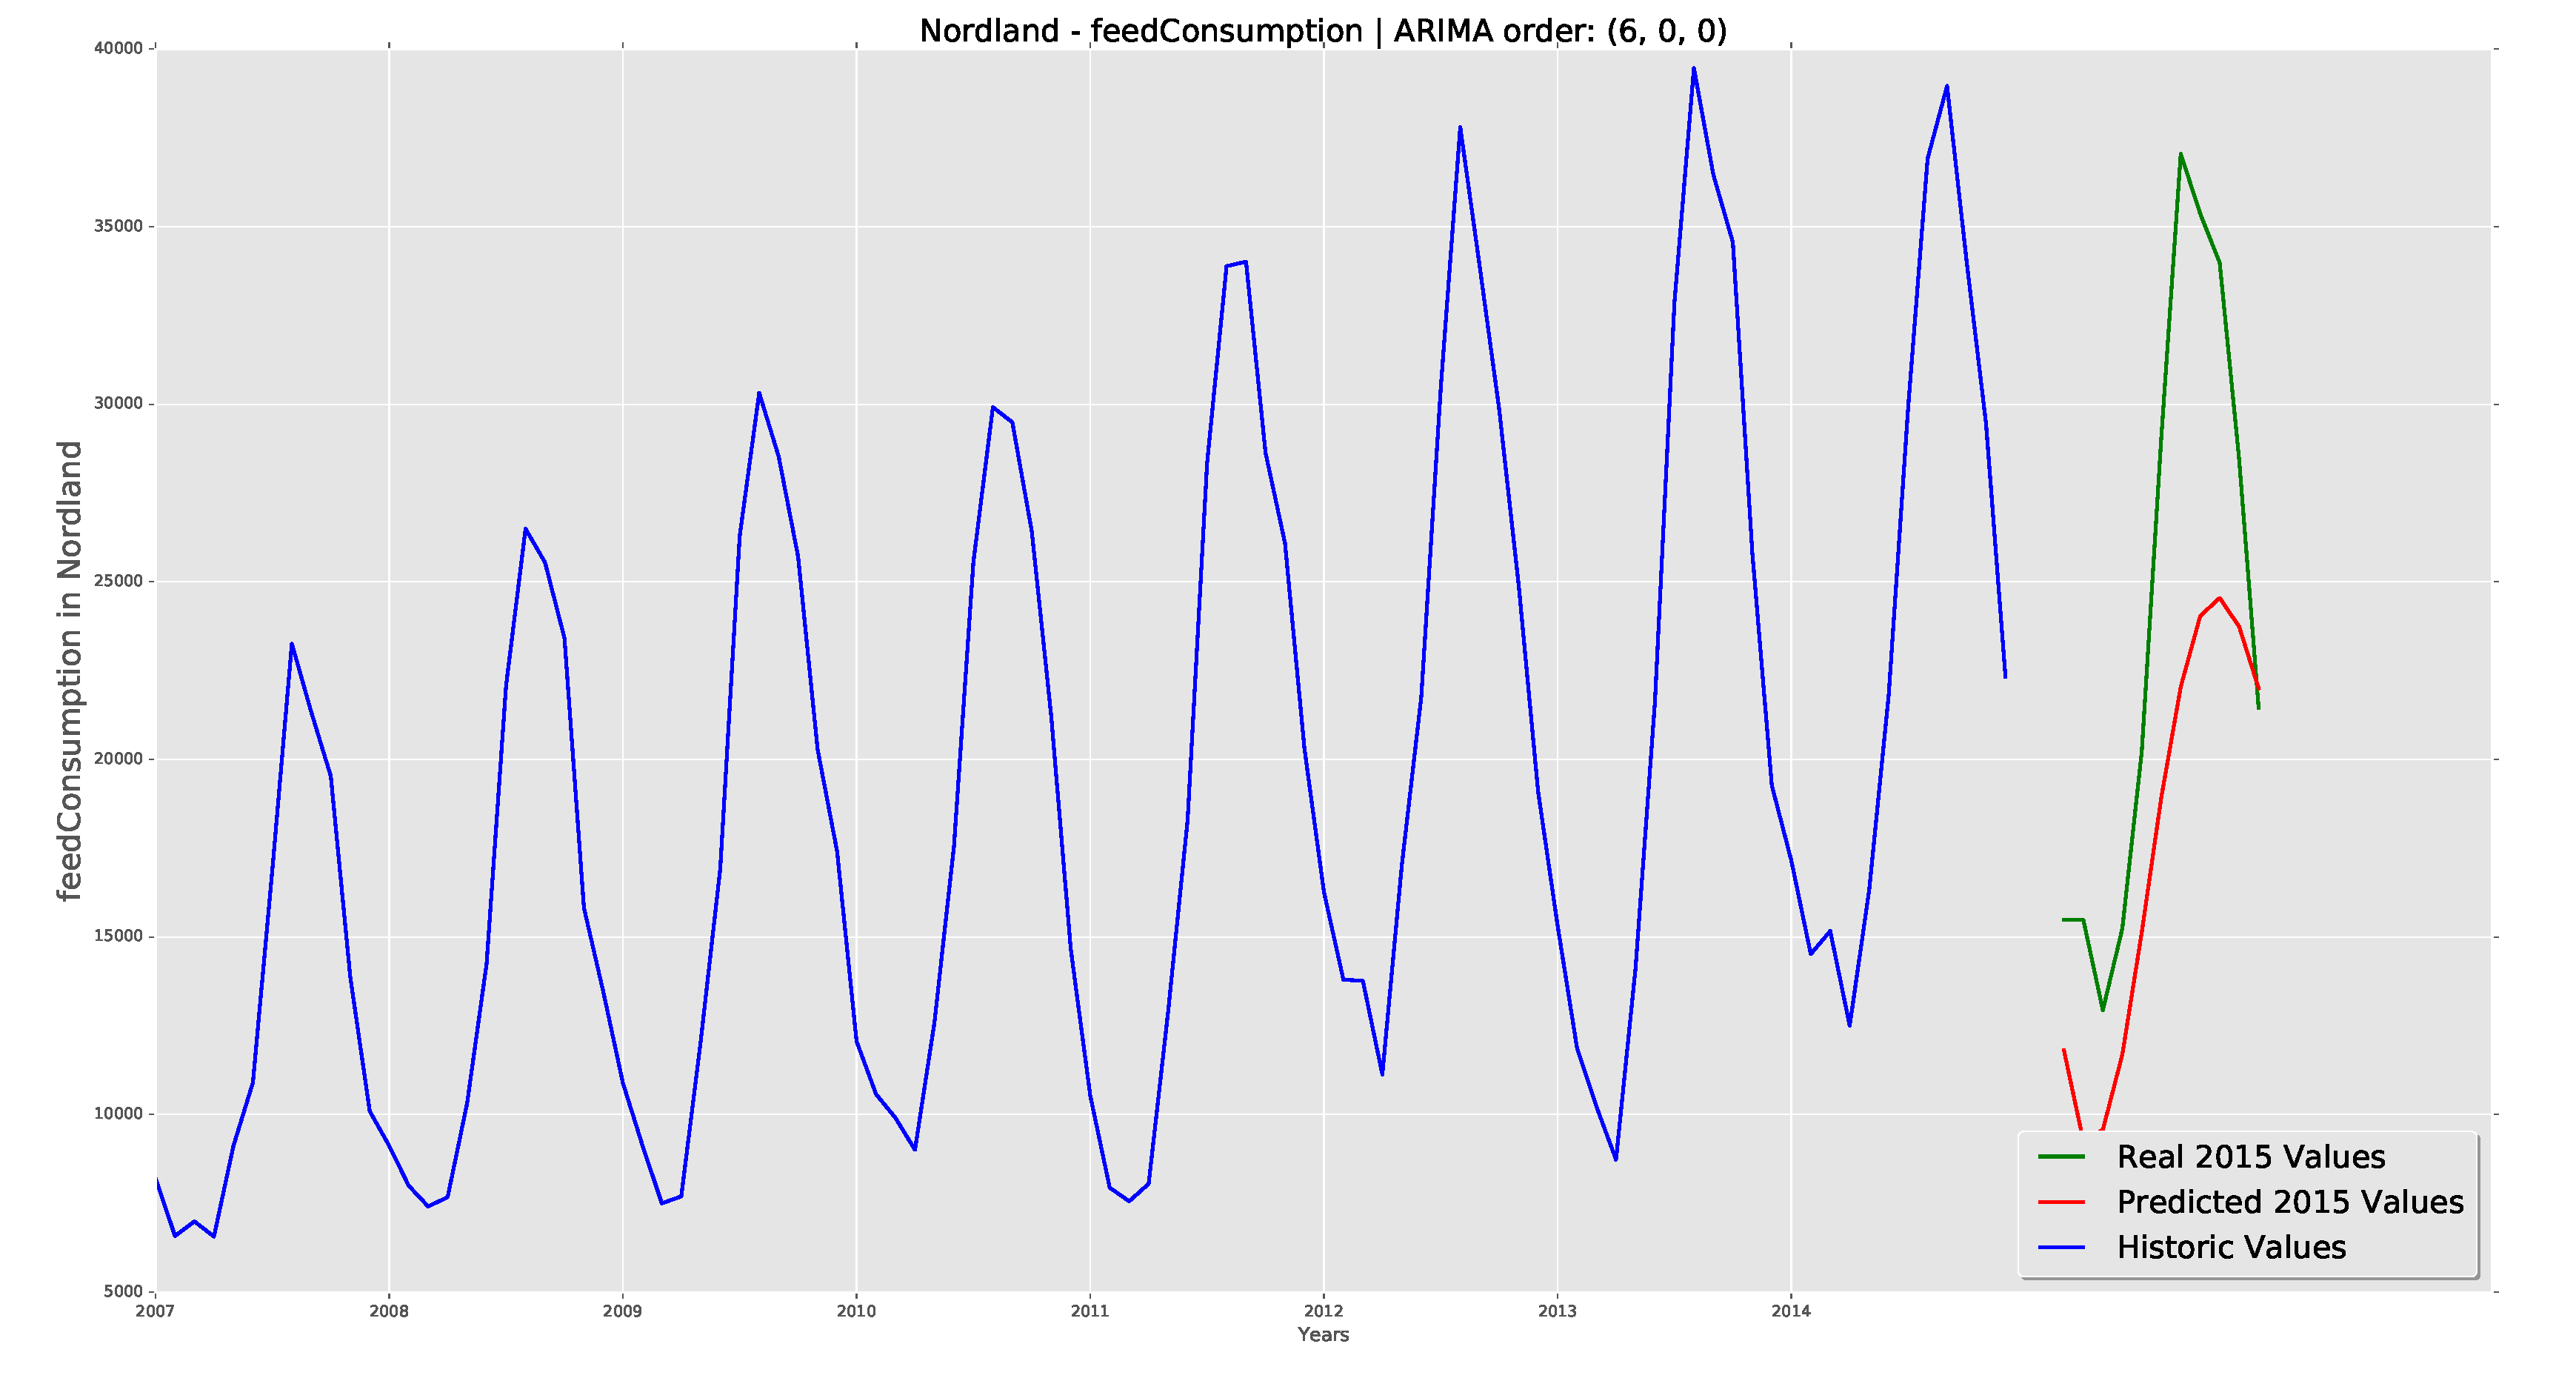
\includegraphics[trim={0 1cm 0 0},clip,width=1.3\textwidth]{Files/Nordland-feedConsumption_pred.pdf}}
    \caption[Predicted 2015 feed consumption in Nordland. Evaluation system ARIMA order.]{Predictions of 2015 feed consumption values in Nordland using ARIMA model fitted with the order suggested by the evaluation system results (6,0,0).\\  It provides an average MAPE of 26.01\% between the real and predicted 2015 values. }
    \label{fig: Nordland_ARIMAevaluation}
\end{figure}

\begin{figure}[H]
	\makebox[\textwidth][c]{
    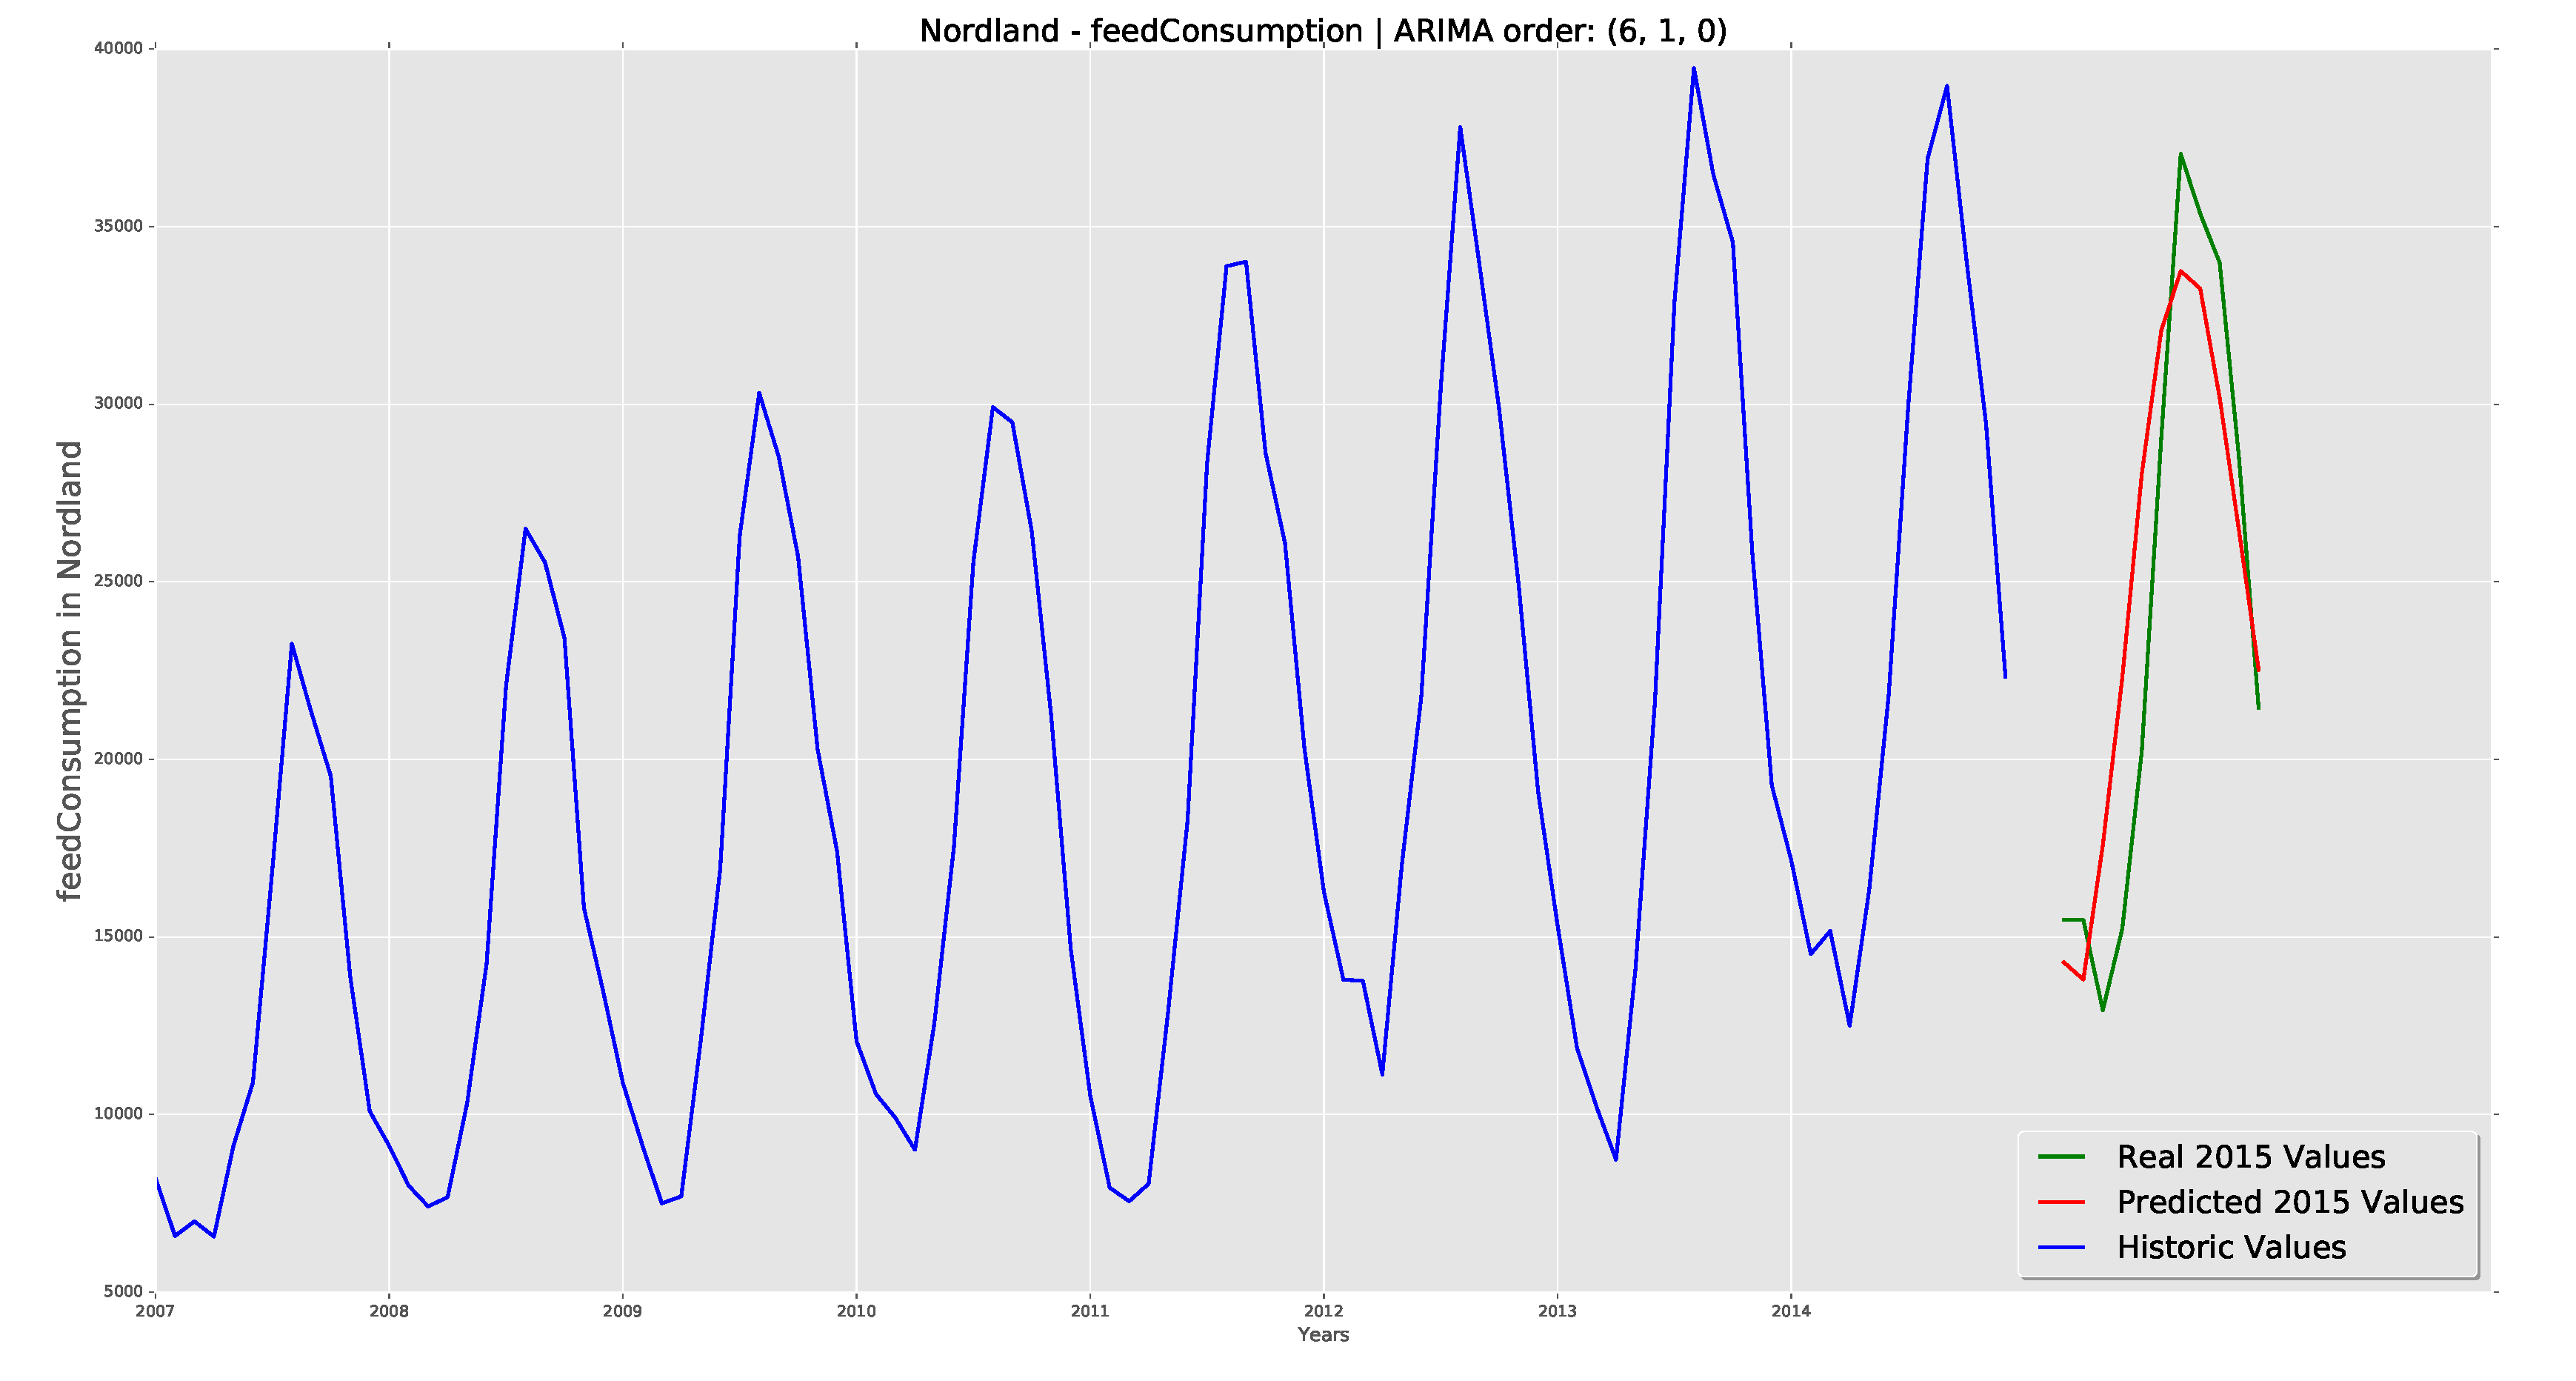
\includegraphics[trim={0 1cm 0 0},clip,width=1.3\textwidth]{Files/Nordland-feedConsumption_BETTER.pdf}}
    \caption[Predicted 2015 feed consumption in Nordland. Manual ARIMA order.]{Predictions of 2015 feed consumption values in Nordland using ARIMA model fitted with an order manually chosen (6,1,0).\\  It provides an average MAPE of 16.82\% between the real and predicted 2015 values. }
    \label{fig: Nordland_ARIMAmanual}
\end{figure}


\newpage

\section{Improvements for feed consumption forecasting }
During the implementation of this work, was also noticed a strong relation between the two parameters "Sea Average Temperature" and "Feed Consumption".
I decided to focus on this particular correlation because, also if it's already well known that is possible to feed more the salmon when the temperature is higher, it could be very useful for further predictions about feed consumption values, since the sea average temperature would be considered like a parameter to use for improve the final results.

This correlation is significant for all the Norwegian counties and it's clearly possible to see it with the example graphic\footnote{The graphics reported above have been displayed with a Python system implemented during this study, that allows to display different parameters in a normalized range. The system has not been reported in the thesis work, but is possible to find it here named "Analysis.py": \\ \url{https://github.com/Sprea22/Personal_Utilities}} reported below here. 

\vspace{-10mm}

\makebox[1\textwidth][c]{
\begin{minipage}[t]{0.6\textwidth}
\begin{figure}[H]
    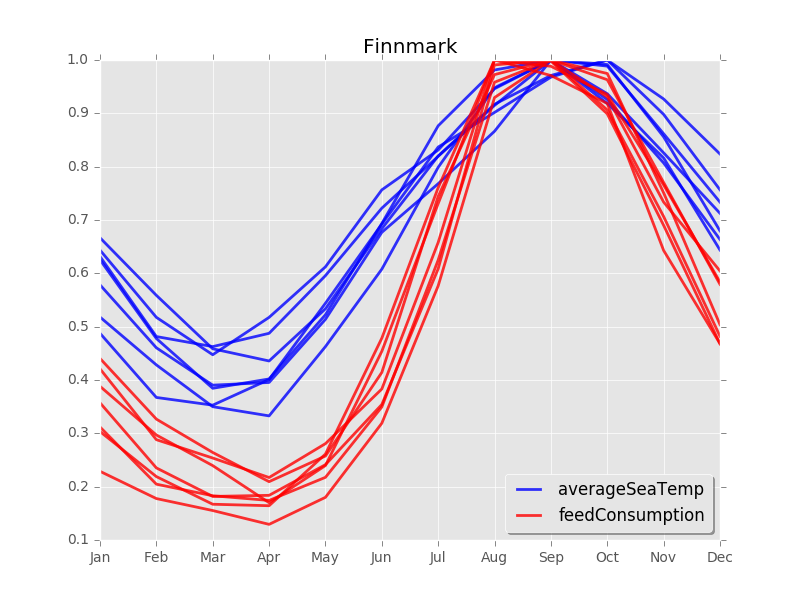
\includegraphics[trim={0 0.5cm 0 0},clip,width=1\textwidth]{Files/Finnmark-Temp&Feed.png}
    \caption[Finnmark: average sea temperature compared with feed consumption]{Comparison between average sea temperature and feed consumption in Finnmark}
    \label{fig: Finnmark_seaTemp&feed}
\end{figure}
\end{minipage} \hfill
\begin{minipage}[t]{0.6\textwidth}
\begin{figure}[H]
	\centering
    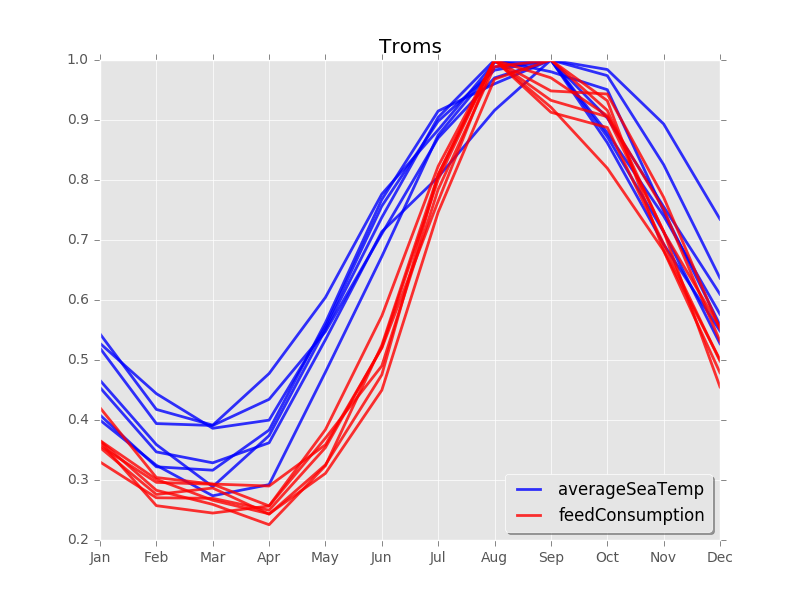
\includegraphics[trim={0 0.5cm 0 0},clip,width=1\textwidth]{Files/Troms-Temp&Feed.png}
    \caption[Troms: average sea temperature compared with feed consumption]{Comparison between average sea temperature and feed consumption in Troms}
    \label{fig: Troms_seaTemp&feed}
\end{figure}
\end{minipage}}
\makebox[1\textwidth][c]{
\begin{minipage}[t]{0.6\textwidth}
\begin{figure}[H]
    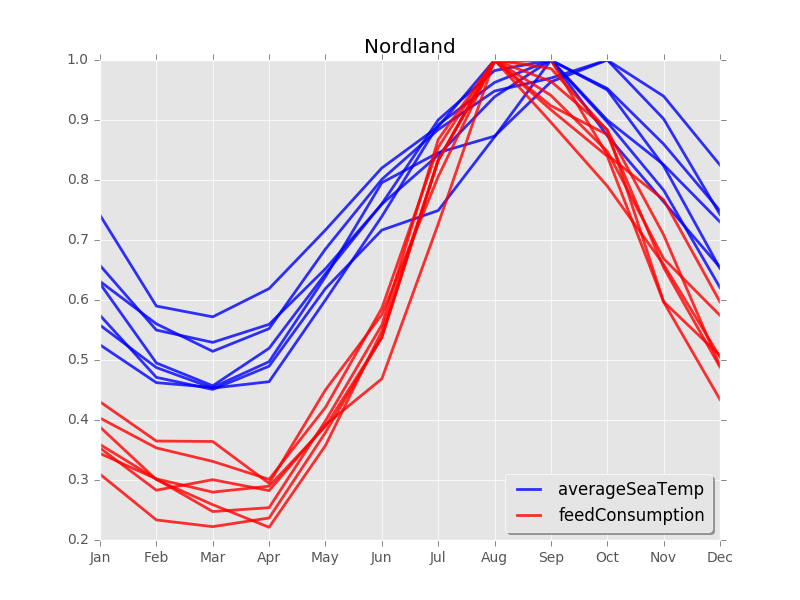
\includegraphics[trim={0 0.5cm 0 1cm},clip,width=1\textwidth]{Files/Nordland-Temp&Feed.png}
    \caption[Nordland: average sea temperature compared with feed consumption]{Comparison betwen average sea temperature and feed consumption in Nordland}
    \label{fig: Nordland_seaTemp&feed}
\end{figure}
\end{minipage} \hfill
\begin{minipage}[t]{0.6\textwidth}
\begin{figure}[H]
	\centering
    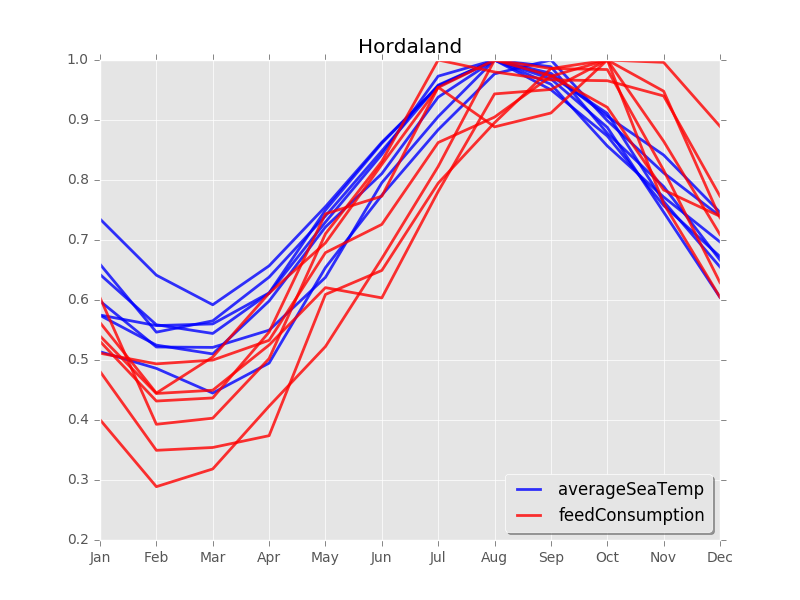
\includegraphics[trim={0 0.5cm 0 1cm},clip,width=1\textwidth]{Files/Hordaland-Temp&Feed.png}
    \caption[Hordaland: average sea temperature compared with feed consumption]{Comparison between average sea temperature and feed consumption in Hordaland}
    \label{fig: Hordaland_seaTemp&feed}
\end{figure}
\end{minipage}}

\newpage

The following graphics allow to have a very clear overview of what just written above.\\
\vspace{-10mm}
\begin{itemize}
 \setlength{\itemsep}{-5pt}
 \item In the first graphic is reported the average sea temperature, where blue means lower temperature and red higher temperature.
 \item In the second graphic is reported the feed consumption per biomass, where red means an higher consumption and blue a lower one.
\end{itemize}

So it's clearly possible to see how the average sea temperature and the feed consumption per biomass have a significant correlation for every single Norwegian county.

\begin{figure}[H]
	\makebox[\textwidth][c]{
    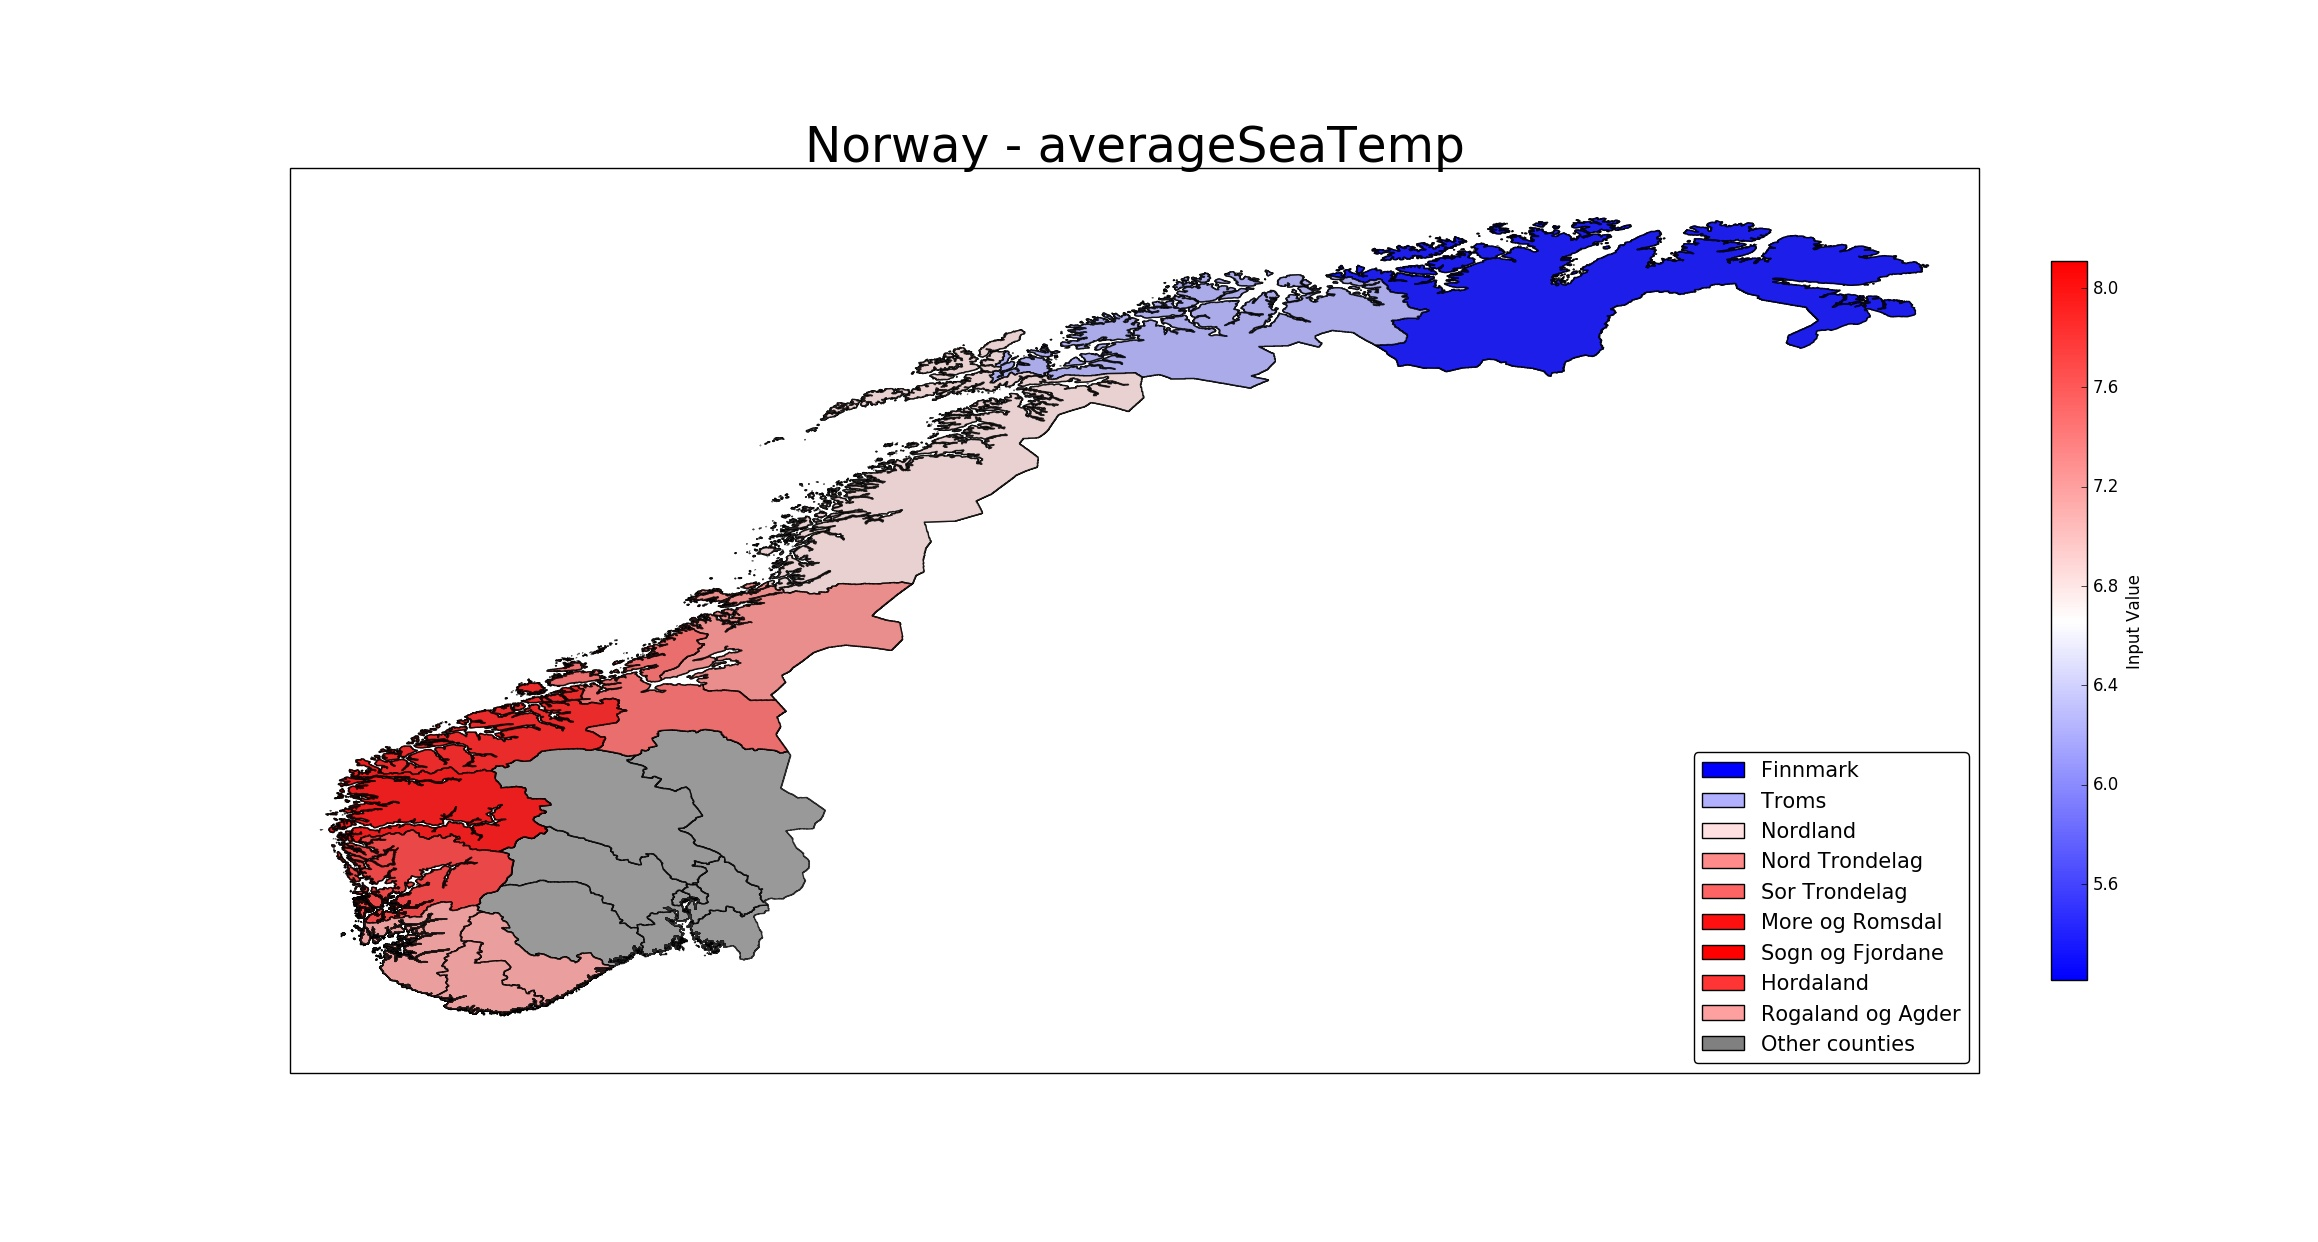
\includegraphics[trim={0 4cm 0 3cm},clip,width=1.3\textwidth]{Files/norway_averageSeaTemp.pdf}}
    \caption{Monthly average sea temperature from 2007 to 2014 in Norway}
    \label{fig: Norway_averageSeaTemp}
\end{figure}

\begin{figure}[H]
	\makebox[\textwidth][c]{
    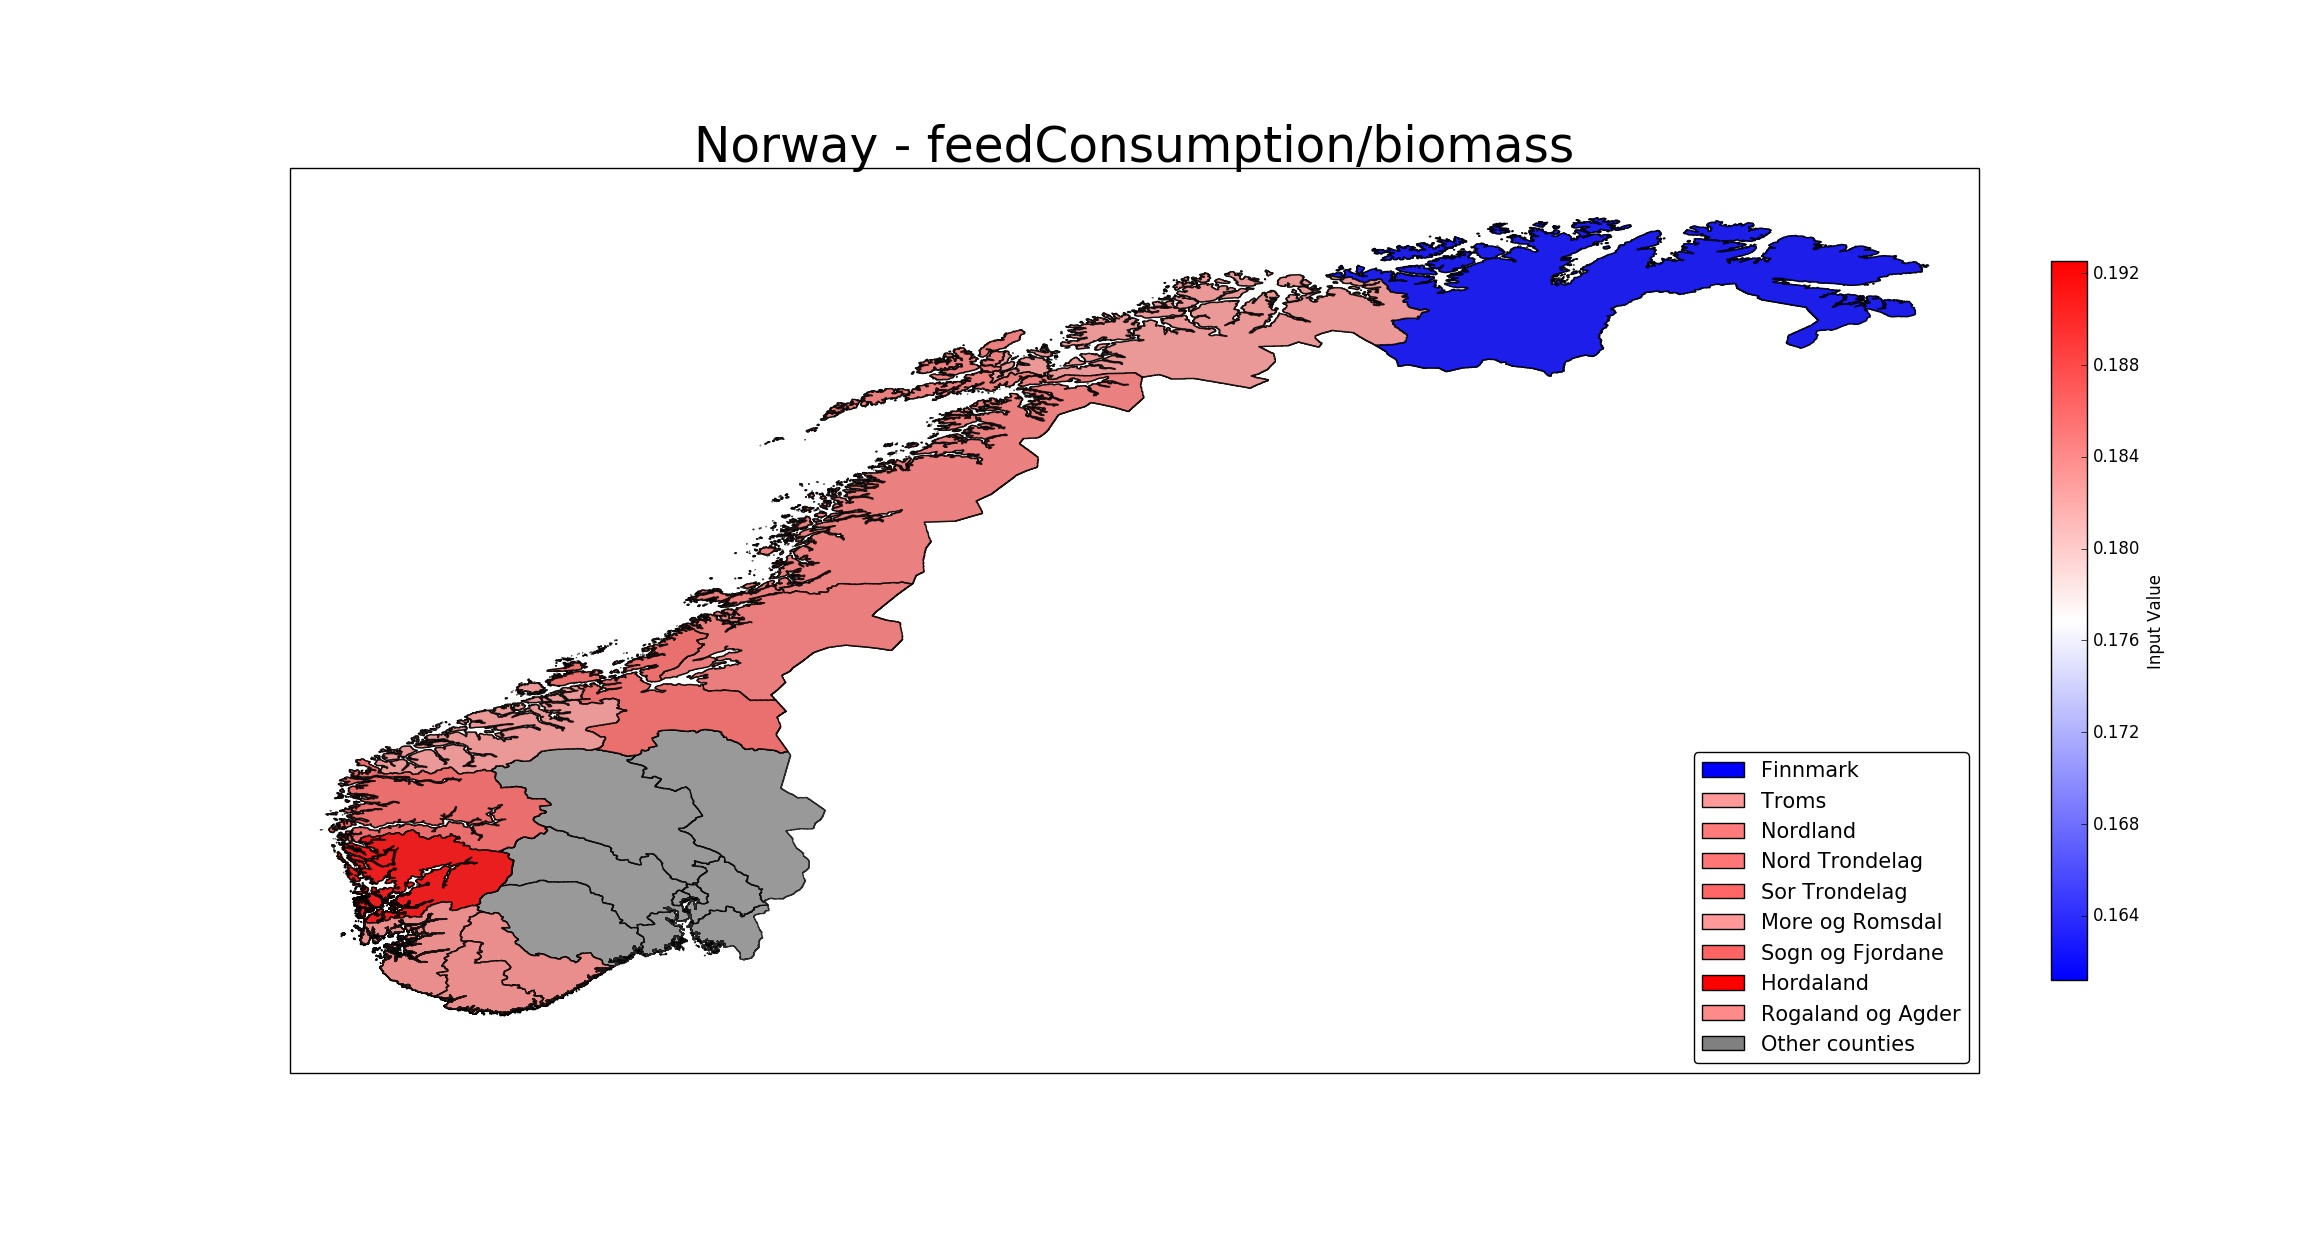
\includegraphics[trim={0 4cm 0 3cm},clip,width=1.3\textwidth]{Files/norway_feed-biomass.pdf}}
    \caption{Monthly average feed consumption per biomass from 2007 to 2014 in Norway}
    \label{fig: Norway_feed-biomass}
\end{figure}

\newpage

Furthermore, is even possible to check the correlation coefficient values reported in the correlation matrix below here. These graphic represent the correlation coefficient between different parameter about the same dataset (county in this case).\\
It's possible to see how the "feedConsumption" and "averageSeaTemp" correlation value is representing an high correlation between the two parameters in example datasets reported here and, if you check through the other counties graphics, this correlation is valid for all the Norwegian counties.\\  \vspace{-15mm}

\makebox[1\textwidth][c]{
\begin{minipage}[t]{0.6\textwidth}
\begin{figure}[H]
    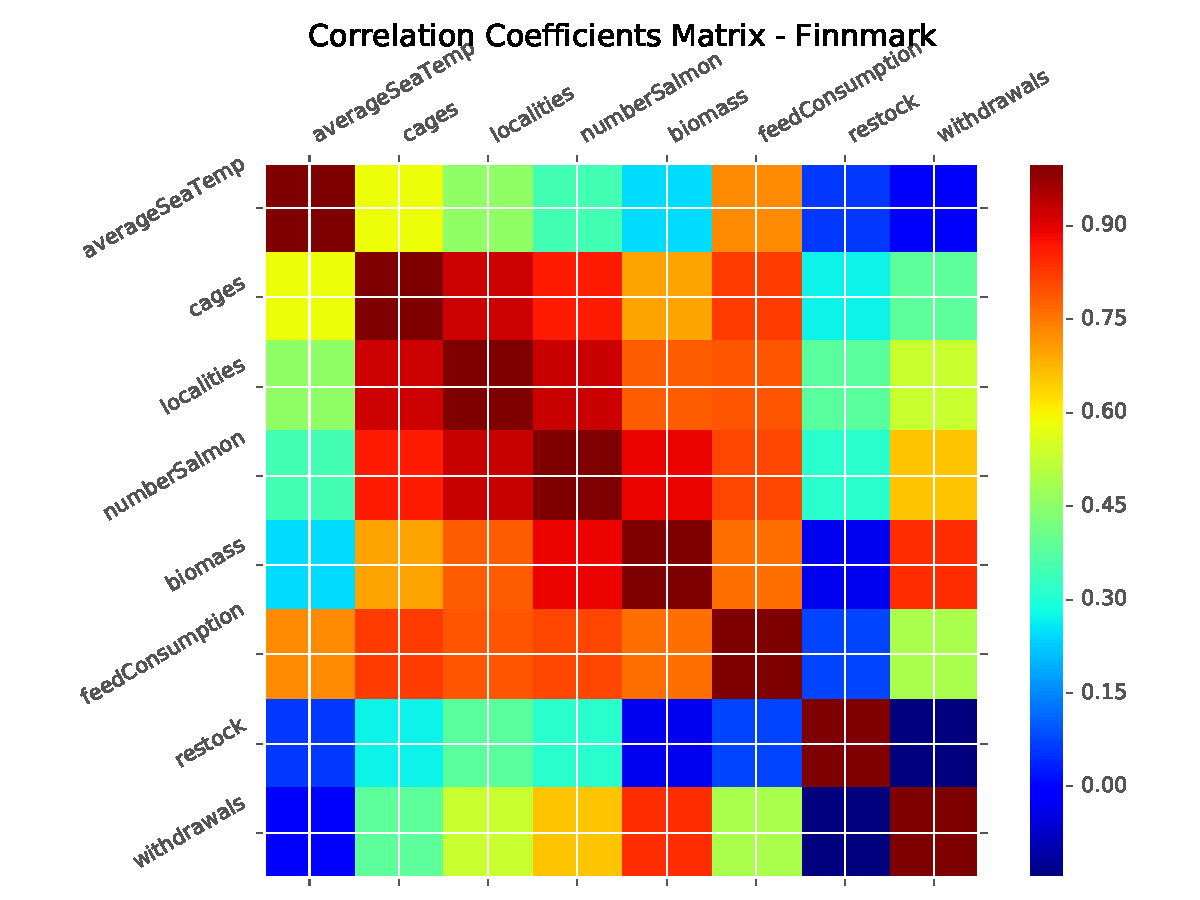
\includegraphics[trim={0 0 0 0},clip,width=1\textwidth]{Files/Finnmark_Total_Matrix.pdf}
    \caption[Correlation matrix between parameter of Finnmark dataset.]{Correlation matrix between all the parameters of the dataset about Finnmark}
    \label{fig: Finnmark_parametersComparison}
\end{figure}
\end{minipage} \hfill
\begin{minipage}[t]{0.6\textwidth}
\begin{figure}[H]
	\centering
    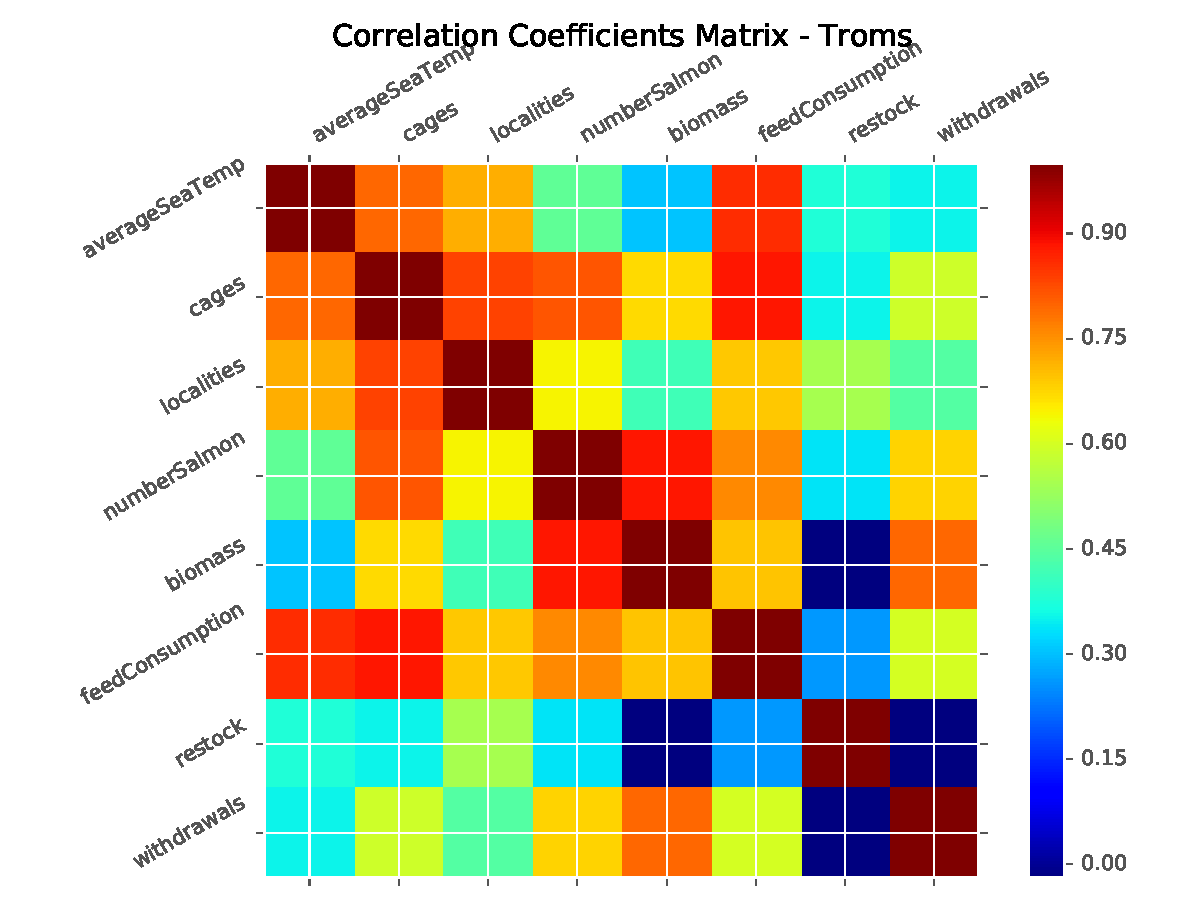
\includegraphics[trim={0 0 0 0},clip,width=1\textwidth]{Files/Troms_Total_Matrix.pdf}
    \caption[Correlation matrix between parameter of Troms dataset.]{Correlation matrix between all the parameters of the dataset about Troms}
    \label{fig: Troms_parametersComparison}
\end{figure}
\end{minipage}}
\makebox[1\textwidth][c]{
\begin{minipage}[t]{0.6\textwidth}
\begin{figure}[H]
    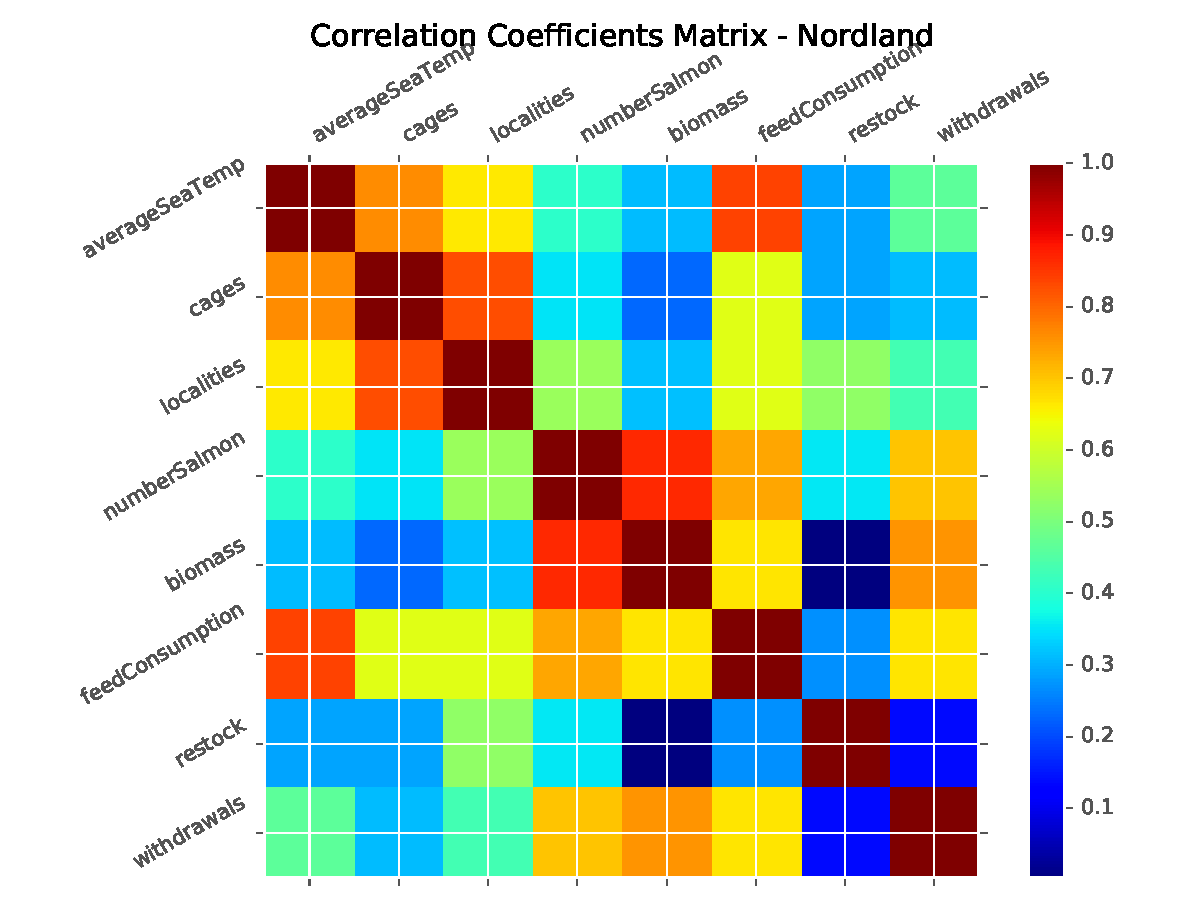
\includegraphics[trim={0 0 0 0},clip,width=1\textwidth]{Files/Nordland_Total_Matrix.pdf}
    \caption[Correlation matrix between parameter of Nordland dataset.]{Correlation matrix between all the parameters of the dataset about Nordland}
    \label{fig: Nordland_parametersComparison}
\end{figure}
\end{minipage} \hfill
\begin{minipage}[t]{0.6\textwidth}
\begin{figure}[H]
	\centering
    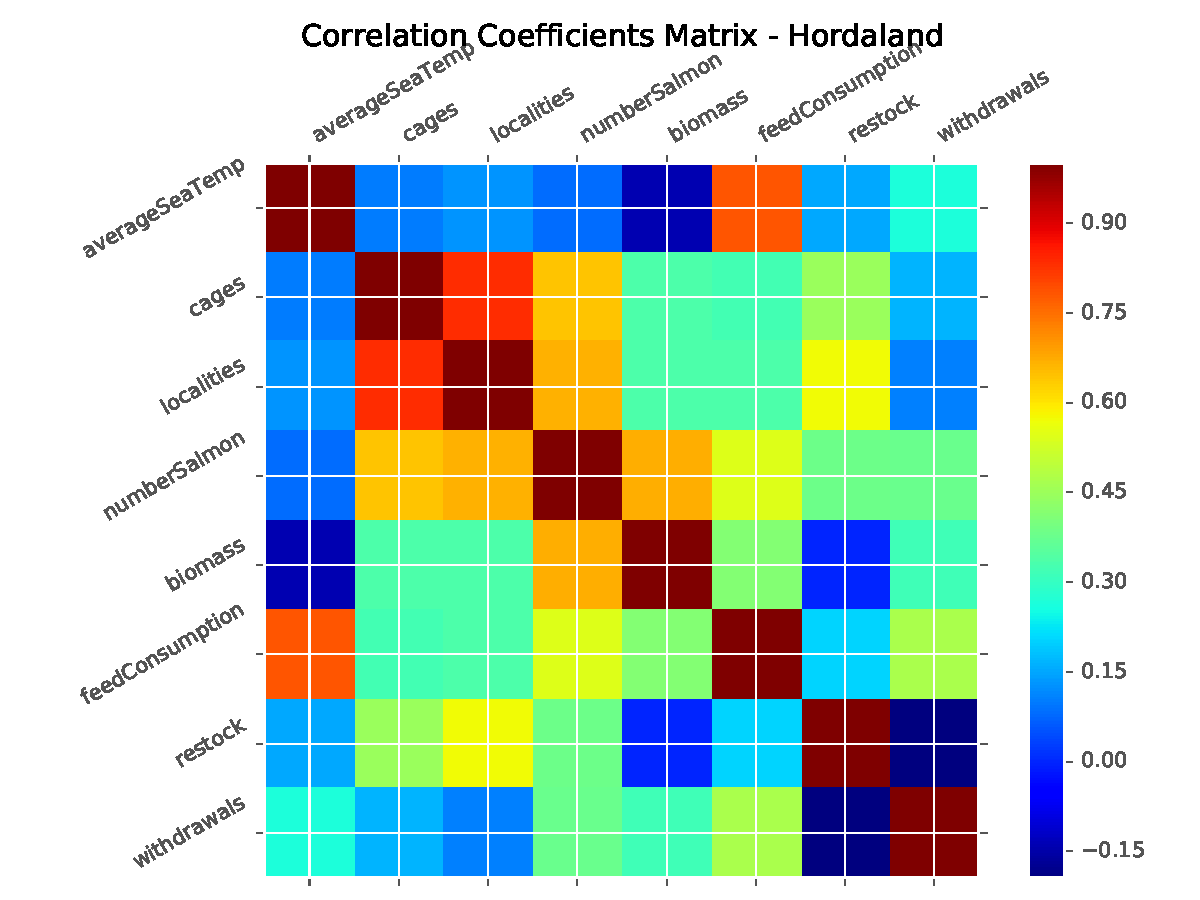
\includegraphics[trim={0 0 0 0},clip,width=1\textwidth]{Files/Hordaland_Total_Matrix.pdf}
    \caption[Correlation matrix between parameter of Hordaland dataset.]{Correlation matrix between all the parameters of the dataset about Hordaland}
    \label{fig: Hordaland_parametersComparison}
\end{figure}
\end{minipage}}



 % Evaluations
\chap{Conclusion}

\section{Summary}


\section{Recommendations to future work}
\subsection{Improve the dataset content}
\subsection{Visualization of the data}
\subsection{Improve the prediction system}
\subsection{System as a service}
This system has been developed with the idea that it could become a "Service system", that is basically a configuration of technology and organizational networks designed to deliver services that satisfy the needs or wants of customers.
Since the prediction system implemented during this work is almost 100\% reusable, it could be used from people for prediction about any kind of data. 

Basically the idea is to create a web application that allows to let you upload your own dataset, choose your own preferences and prediction settings, and then the system will calculate and display prediction of the current values in the future together with the MAPE (Mean Average Percentage Error) to have an idea bout how accurate are the.\\


\begin{figure}[H]
	\centering
        \makebox[\textwidth][c]{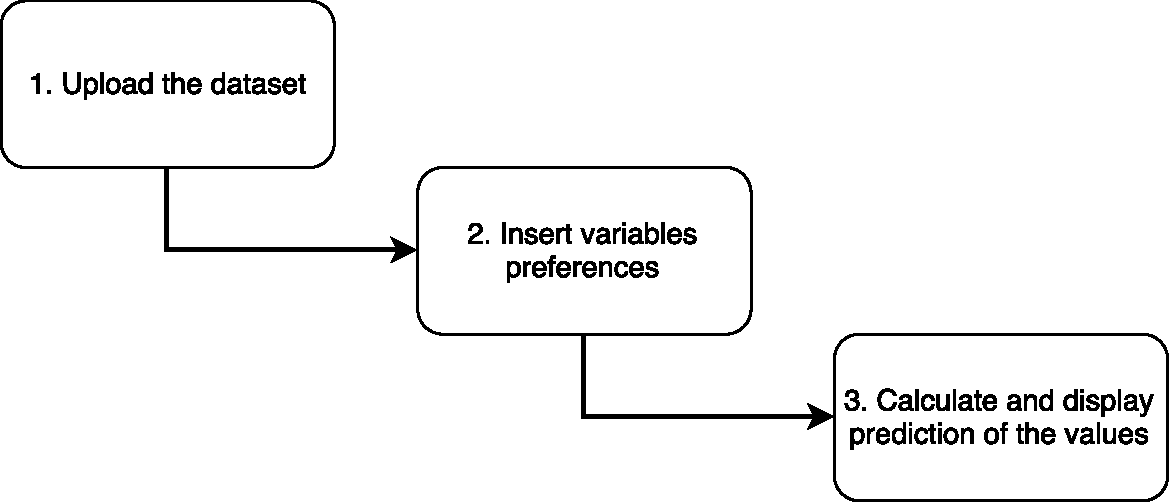
\includegraphics[width=1\textwidth]{Files/ServiceSystem.pdf}}
    \caption{Idea of the Servie System for predictions.}
\end{figure}







 % Conclusion

%
\chapter{Recommendations to future work}
\section{Dataset about single locality}
This thesis allows to have a general overview and predictions of values about the aquaculture business in Norway. 

But it would be much more useful, in particular for people into the aquaculture business, to use this system to have an overview and predictions of data provided by a single locality of aquaculture.\\
In this case the system could be used from the owner of the locality to analyze historic values and use the prediction system to have a forecast about some particular parameters.

\section{Visualization of the data}

\section{Test prediction system with a bigger dataset}

\newpage

\section{Prediction system as a service}
This system has been developed with the idea that it could become a "Service system", that is basically a configuration of technology and organizational networks designed to deliver services that satisfy the needs or wants of customers.
Since the prediction system implemented during this work is almost 100\% reusable, it could be used from people for prediction about any kind of data. 

Basically the idea is to create a web application that allows to let you upload your own dataset, choose your own preferences and prediction settings, and then the system will calculate and display prediction of the current values in the future together with the MAPE (Mean Average Percentage Error) to have an idea bout how accurate are the.\\


\begin{figure}[H]
	\centering
        \makebox[\textwidth][c]{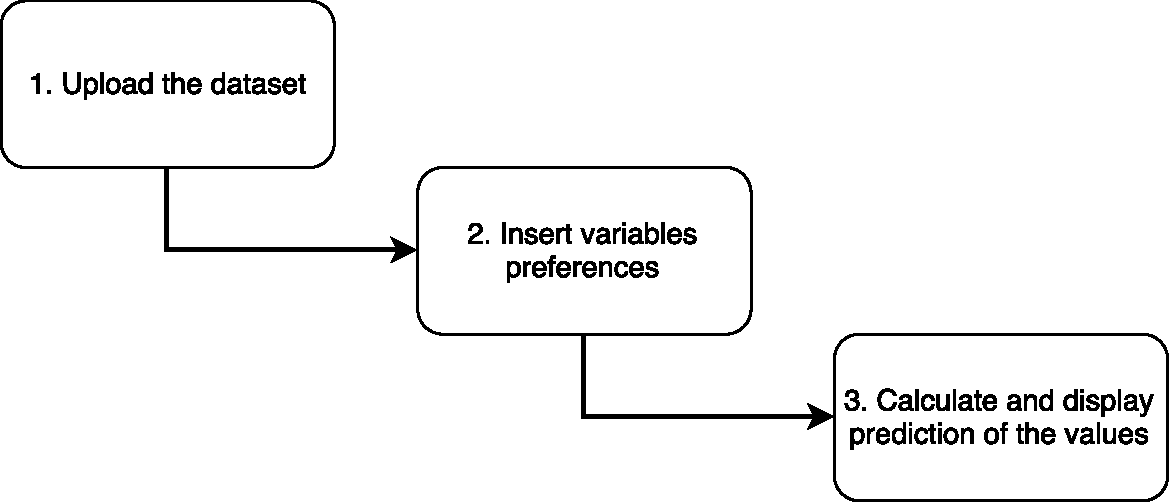
\includegraphics[width=1\textwidth]{Files/ServiceSystem.pdf}}
    \caption{Idea of the Servie System for predictions.}
\end{figure}








%% Appendices -----------------------------------------------------
\addtocontents{toc}{\vspace{2em}} % Add a gap in the Contents, for aesthetics

\lhead{\emph{Appendices}}  % Change the left side page header to "Appendices"

\part{Full Code Implementation}
\begin{appendix}

\chap{SIA Implementation code}

\section{SIA: Imported libraries}
\label{SIA_libraries}
The library "os" is really important since provides a waay of using operating system dependent functinality.
\begin{lstlisting}
import os
\end{lstlisting}

Also the library "sys" would be very useful for test and execute the program, mainly because it allows to input directly from terminal.
\begin{lstlisting}
import sys
\end{lstlisting}

The "pylab" library will be useful for plot data.
\begin{lstlisting}
import pylab
\end{lstlisting}

The "pandas" library will be very useful for read the data from CSV dataset and setup the plot abut it.
\begin{lstlisting}
import pandas as pd
\end{lstlisting}

The "numpy" library it's used for mathematic purpose, such as calculating the correlation coefficent between two series.
\begin{lstlisting}
import numpy as np
\end{lstlisting}
 
The "pyplot" library it's used for basic graphic displaying and customization, easy to use but very efficent.
\begin{lstlisting}
import matplotlib.pyplot as pyplot
\end{lstlisting}

The library "PIL" supports many file formats, and provides powerful image processing and graphics capabilities.
\begin{lstlisting}
from PIL import Image
\end{lstlisting}

The library "fpdf" allows to generate and use PDF file.
\begin{lstlisting}
from fpdf import FPDF
\end{lstlisting}

\section{SIA section I: Total graphic for all the years}
\label{SIA_section_I}
\textbf{Code implementation:}\\
During this section of the code was used "pandas" library for read the dataset.
\begin{lstlisting}
series = pd.read_csv("Dataset.csv", usecols=[1,sys.argv[1]])
\end{lstlisting}

Then using the "pyplot" library has been possible to setup the plot of the input data.
\begin{lstlisting}
series.plot(color="blue", linewidth=1.5)
\end{lstlisting}


Thera are some settings about the axis x just to display the data in the right format, are easy to change and to costume.
\begin{lstlisting}
years = ["2005","2006","2007","2008","2009","2010",
	"2011","2012","2013","2014","2015","2016"]
x = range(144)
pyplot.xticks(np.arange(min(x), max(x)+1, 12.0), years)
pyplot.title("Total graphic from 2005 to 2016")
\end{lstlisting}

Once setted up the plot of the current data, the next step was to display the trendline of the current graphic. \\ 
The following code represent the method for calculate and display it.
\begin{lstlisting}
def trendline(x, y, col):
	z = np.polyfit(x, y, 1)
	p = np.poly1d(z)
	pylab.plot(x,p(x), c=col)
	# print "y=%.6fx+(%.6f)"%(z[0],z[1])
\end{lstlisting}	

At this point the current data values have been read again and passed to the method just impleneted above for calculating the trendline.
\begin{lstlisting}
series2 = pd.read_csv("Dataset.csv", usecols=[sys.argv[1]],
			squeeze=True)
trendline(x, seriesV.values, "red")
\end{lstlisting}

There is the possibility to save the graphic like an image and/or display it.
\begin{lstlisting}
saveFigure("_Total.jpg")
\end{lstlisting}


\section{SIA section II: Single graphics for each year}
\label{SIA_section_II}
\textbf{Code implementation:}\\
During this section of the code was used "pandas" library for read the dataset.
\begin{lstlisting}
series2 = pd.read_csv("Dataset.csv", index_col=['Month'],
			usecols=[0,1,sys.argv[1]])
\end{lstlisting}

Some initialization of variables that are going to be useful.
\begin{lstlisting}
months = ["Jan","Feb","Mar","Apr","May","Jun",
		"Jul","Aug","Sep","Oct","Nov","Dec"]
x_pos = np.arange(len(months))
test = []
j = 0
\end{lstlisting}

The following code allows the system to split the values and display them in the right way: that means that are going to be splitted for each single year and then plotted on the same graphic.
\begin{lstlisting}
for i in range(len(series2.values)):
	if j in range(12):
		test.append(series2.values[i][1])
		j = j + 1
	else:
		pyplot.plot(x_pos, test, linewidth=2, 
			alpha=0.8, 
			label = int(series2.values[i-1][0]))
		test = []
		test.append(series2.values[i][1])
		j = 1

\end{lstlisting}

These are some personalization settings that could be easily changed as you want.
\begin{lstlisting}
ax.legend(loc=4, ncol=1, fancybox=True, shadow=True)
pyplot.xticks(x_pos,months)
pyplot.xlim(0,11)
pyplot.title(sys.argv[1]+ 
		": Single year's graphic from 2005 to 2016")
\end{lstlisting}

There is the possibility to save the graphic like an image and/or display it.
\begin{lstlisting}
saveFigure("_Years.jpg")
\end{lstlisting}


\section{SIA section III: Correlation matrix between years}
\label{SIA_section_III}
\textbf{Code implementation:}\\
During this section of the code was used "pandas" library for read the dataset.
\begin{lstlisting}
series3 = pd.read_csv("Dataset.csv", index_col=['Year'],
			usecols=[0,sys.argv[1]])
\end{lstlisting}

\begin{lstlisting}
corr = []
test = []
j = 0
# Collecting the correct values to elaborate.
for i in range(len(series2.values)+1):
	if j in range(12):
		test.append(series2.values[i][1])
		j = j + 1
	else:
		corr.append(test)
		test = []
		if i in range(144):
			test.append(series2.values[i][1])
			j = 1
\end{lstlisting}

With the library "numpy" is possible to calculate the correlation coefficents between all the variables in the series just read.
\begin{lstlisting}
test = np.corrcoef(corr)
\end{lstlisting}

Setup the figure that will display the correlation matrix using the library "pypot".
\begin{lstlisting}
fig2 = pyplot.figure()
ax = fig2.add_subplot(111)
\end{lstlisting}

Creating the correlation matrix using the already calculated correlation coefficents.
\begin{lstlisting}
cax = ax.matshow(test, interpolation='nearest')
\end{lstlisting}

Settings for display the matrix in the right way, in particular for the values to display on both the axis x and y, in this case every single year from 2005 to 2016
\begin{lstlisting}
pyplot.title(sys.argv[1]+ ": Correlation between different years")
years = ["2005","2006","2007","2008","2009","2010",
	"2011","2012","2013","2014","2015","2016"]
x_pos = np.arange(len(years))
y_pos = np.arange(len(years))
pyplot.yticks(y_pos,years)
pyplot.xticks(x_pos,years)
pyplot.colorbar(cax)
\end{lstlisting}
\newpage
Adding a title to the graphic that we are going to display and also a bar that works like a legend for the colors of the matrix, allowing the reader to better understand the values reported inside the matrix.
\begin{lstlisting}
saveFigure("_Years_Matrix.jpg")
\end{lstlisting}

There is the possibility to save the correlation matrix like an image and/or display it.
\begin{lstlisting}
pyplot.savefig("OUTPUT_DIRECTORY", format="jpg")
pyplot.show()
\end{lstlisting}


\section{SIA section IV: Correlation matrix between months}
\label{SIA_section_IV}
\textbf{Code implementation:}\\
During this section of the code was used "pandas" library for read the dataset.
\begin{lstlisting}
series4 = pd.read_csv("Dataset.csv", usecols=[0,1,sys.argv[1]])
\end{lstlisting}

\begin{lstlisting}
corr = []
for Month, Year in series4.groupby(["Month"], sort=False):
	corr.append(Year[sys.argv[1]].values)
\end{lstlisting}
	
With the library "numpy" is possible to calculate the correlation coefficents between all the variables in the series just read.
\begin{lstlisting}
test = np.corrcoef(series4.values)
\end{lstlisting}

Setup the figure that will display the correlation matrix using the library "pypot".
\begin{lstlisting}
fig2 = pyplot.figure()
ax = fig2.add_subplot(111)
\end{lstlisting}

Creating the correlation matrix using the already calculated correlation coefficents.
\begin{lstlisting}
cax = ax.matshow(test, interpolation='nearest')
\end{lstlisting}

Settings for display the matrix in the right way, in particular for the values to display on both the axis x and y, in this case every single months of the year.
\begin{lstlisting}
months = ["Jan","Feb","Mar","Apr","May","Jun",
	"Jul","Aug","Sep","Oct","Nov","Dec"]
x_pos = np.arange(len(months))
y_pos = np.arange(len(months))
pyplot.yticks(y_pos,months)
pyplot.xticks(x_pos,months)
\end{lstlisting}
Adding a title to the graphic that we are going to display and also a bar that works like a legend for the colors of the matrix, allowing the reader to better understand the values reported inside the matrix.
\begin{lstlisting}
pyplot.title("Correlation between different months")
pyplot.colorbar(cax)
\end{lstlisting}

There is the possibility to save the correlation matrix like an image and/or display it.
\begin{lstlisting}
saveFigure("_Months_Matrix.jpg")
pyplot.show()
\end{lstlisting}

\section{SIA section V: Single overview}
\label{SIA_section_V}
\textbf{Code implementation:}\\
create\_single\_overview() : this method will use the "Image" library for autogenerate a collage of the current input's graphics and save it like an overview image. The content of the params will basically decide how the "Current input overview image" will looks like.

It uses each single "current input overview image" of all the inputs and the "correlation matrix between all the inputs image" for combine them in a unique "total overview" and save it using the PDF format.

\begin{lstlisting}
listofimages=["CURRENT_INPUT_TOTAL_GRAPHIC",
            "CURRENT_INPUT_YEARS_MATRIX", 
            "CURRENT_INPUT_YEARS_GRAPHIC",
            "CURRENT_INPUT_MONTHS_MATRIX"]
            
create_single_overview(params1, listofimages)
create_single_overview(params2, listofimages)
\end{lstlisting}


The "create\_single\_overview" method has basically this structured, and then its configuration depends from the input data and from the preferences.
\begin{lstlisting}
def create_single_overview(cols, rows ,
			width, height, listofimages):
    thumbnail_width = width//cols
    thumbnail_height = height//rows
    size = thumbnail_width, thumbnail_height
    new_im = Image.new('RGB', (width, height))
    ims = []
    for p in listofimages:
        im = Image.open(p)
        im.thumbnail(size)
        ims.append(im)
    i = 0
    x = 0
    y = 0
    for col in range(cols):
        for row in range(rows):
            new_im.paste(ims[i], (x, y))
            i += 1
            y += thumbnail_height
        x += thumbnail_width
        y = 0
    new_im.save(SINGLE_OVERVIEW_IMAGE")
	new_im.show()
\end{lstlisting}
 % SIA Implementation code

\chap{MIA Implementation code}
\label{MIA_Implementation}
\section{MIA: Imported libraries}
\label{MIA_Libraries}
The "pandas" library will be very useful for read the data from CSV dataset and setup the plot abut it.
\begin{lstlisting}
import pandas as pd
\end{lstlisting}

The "numpy" library it's used for mathematic purpose, such as calculating the correlation coefficent between two series.
\begin{lstlisting}
import numpy as np
\end{lstlisting}

 
The "pyplot" library it's used for basic graphic displaying and customization, easy to use but very efficent.
\begin{lstlisting}
import matplotlib.pyplot as pyplot
\end{lstlisting}

\section{MIA: Implementation}
\textbf{Code implementation:}\\
First of all, we are going to use the "pandas" library for read the dataset.
\begin{lstlisting}
series3 = pd.read_csv("TOTAL_DATASET_DIRECTORY", 
	index_col=['Input'], header=0)
\end{lstlisting}

Then with the library "numpy" is possible to calculate the correlation coefficents between all the variables just read above.
\begin{lstlisting}
test = np.corrcoef(series3.values)
\end{lstlisting}

Setup the figure that will display the correlation matrix using the library "pyplot".
\begin{lstlisting}
fig2 = pyplot.figure()
ax = fig2.add_subplot(111)
\end{lstlisting}

Creating the correlationg matrix using the already calculated correlation coefficents.
\begin{lstlisting}
cax = ax.matshow(test, interpolation='nearest')
\end{lstlisting}

Settings for display the matrix in the right way, in particular for the values to display on both the axis x and y, in this case every single input.
\begin{lstlisting}
inputs = ["Cages", "Feed", "Number", "Restock",
	"Local", "Withdr", "Biomass", "Price"]
x_pos = np.arange(len(inputs))
y_pos = np.arange(len(inputs))
pyplot.yticks(y_pos,inputs)
pyplot.xticks(x_pos,inputs)
\end{lstlisting}

Adding a title to the graphic that we are going to display and also a ba that works like a legend for the colors of the matrix, allowing the reader to better understand the values reported inside the matrix.
\begin{lstlisting}
pyplot.title("Correlation between different inputs 
		about data from 2005 to 2016")
pyplot.colorbar(cax)
\end{lstlisting}

In the end, using again the library "pyplot", there is the possibility to save the correlation matrix graphic like an image and/or display it.
\begin{lstlisting}
pyplot.savefig("OUTPUT_DIRECTORY")
\end{lstlisting}

\begin{lstlisting}
series = pd.read_csv("TRENDLINES_VALUES_DOCUMENT",
	 header=0, usecols=["Norm Ang Coeffs"])
series.plot(kind="barh")
pyplot.savefig("OUTPUT_DIRECTORY")

create_total_overview()
\end{lstlisting}

\begin{lstlisting}
pyplot.show()
\end{lstlisting}

 % MIA Implementation code

\chap{Prediction System Implementation code}
\section{Evaluating System}
\section{Training System}
\section{Future Prediction System}

 % Prediction System Implementation code

\chap{Prediction System Implementation code}
\section{Common libraries}
\label{Pred_common_libraries}
\begin{lstlisting}
import os
import sys
import warnings
import numpy as np
import pandas as pd
from pandas import Series
from statsmodels.tsa.arima_model import ARIMA
from sklearn.metrics import mean_squared_error
\end{lstlisting}

\newpage

\section{Common methods}
\label{Pred_common_methods}
\begin{lstlisting}
pyplot.style.use('ggplot')
\end{lstlisting}

\begin{lstlisting}
def mean_absolute_percentage_error(y_true, y_pred): 
	try:
		rng = len(y_true)
		diff = []
		for i in range(0,rng):
			diff.append(y_true[i] - y_pred[i])
			diff[i] = diff[i] / y_true[i]
		abs = np.abs(diff)
		mn = np.mean(abs)
		percentageError = mn * 100
	except:
		rng = 0
		abs = np.abs((y_true-y_pred)/y_true)
		percentageError = abs * 100
	return percentageError
\end{lstlisting}

\newpage

\section{Evaluating System}
\label{Evaluating_System}
Use the common library reported above: [\ref{Pred_common_libraries}] \\
Use the common methods reported above: [\ref{Pred_common_methods}] \\
\begin{lstlisting}
def evaluate_arima_model(X, arima_order):
	train_size = int(len(X) * 0.66)
	train, test = X[0:train_size], X[train_size:]
	history = [x for x in train]
	predictions = list()
	for t in range(len(test)):
		model = ARIMA(history, order=arima_order)
		model_fit = model.fit(disp=0)
		yhat = model_fit.forecast()[0]
		predictions.append(yhat)
		history.append(test[t])
	error = mean_absolute_percentage_error(test, predictions)
	return error
\end{lstlisting}
\begin{lstlisting}
def evaluate_models(dataset, p_values, d_values, q_values):
	dataset = dataset.astype('float32')
	best_score, best_cfg = float("inf"), None
	filename = "Results_Forecast/"+sys.argv[1]+"/"+sys.argv[2]+"_MAPE.csv"
	if not os.path.exists(os.path.dirname(filename)):	
		os.makedirs(os.path.dirname(filename))

	with open(filename, "w") as myfile:
		myfile.write("P, D, Q, MAPE\n")
	for p in p_values:
		for d in d_values:
			for q in q_values:
				order = (p,d,q)
				try:
					mape = evaluate_arima_model(dataset, order)
					with open(filename, "a") as myfile:
						myfile.write('%d, %d, %d, %.3f%% \n' % (p,d,q,mape))
					if mape < best_score:

						best_score, best_cfg = mape, order
					print('ARIMA%s MAPE=%.3f%%' % (order,mape))
				except:
					print('ARIMA%s MAPE=Nil' % str(order))
					continue
	print('Best ARIMA%s MAPE=%.3f%%' % (best_cfg, best_score))
\end{lstlisting}
\begin{lstlisting}
series = pd.read_csv("Datasets/"+sys.argv[1]+".csv", header=0, usecols=[sys.argv[2]])

p_values = [0, 1, 2, 4, 6, 8, 10]
d_values = [0, 1, 2, 3]
q_values = [0, 1, 2, 3]
warnings.filterwarnings("ignore")
evaluate_models(series.values, p_values, d_values, q_values)
\end{lstlisting}

\newpage

\section{Prediction System}
\label{Prediction_System}
Use the common library reported above: [\ref{Pred_common_libraries}] \\
Use the common methods reported above: [\ref{Pred_common_methods}] \\
\begin{lstlisting}
series = pd.read_csv("Datasets/"+sys.argv[1]+".csv", usecols=[sys.argv[2]])
yearInput = pd.read_csv("Datasets/" + sys.argv[1]+".csv", usecols=[0])
realValues = pd.read_csv("Results_Forecast/"+sys.argv[1]+"/"+sys.argv[1]+"_"+sys.argv[2]+"_2015.csv")

realValuesData = realValues[sys.argv[2]].values
realValuesData = realValuesData.astype('float32')
dataset = series.values
dataset = dataset.astype('float32')

p_values = int(sys.argv[4])
d_values = int(sys.argv[5])
q_values = int(sys.argv[6])
order = (p_values, d_values, q_values)
warnings.filterwarnings("ignore")

model = ARIMA(dataset, order=order)
model_fit = model.fit(disp=0)
forecast = model_fit.forecast(int(sys.argv[3]))[0]
\end{lstlisting}
\begin{lstlisting}
index = []
for i in range(1,int(sys.argv[3])+1):
	index.append(len(dataset) +i)
mape_list = []
for i in range(0,len(forecast)):
	mape_list.append(mean_absolute_percentage_error(realValuesData[i], forecast[i]))
rows = zip(index, realValuesData, forecast, mape_list)
f = open("Results_Forecast/"+sys.argv[1]+"/"+sys.argv[1]+"_"+sys.argv[2]+"_futurePred.csv", 'w')
csv.writer(f).writerows(rows)
f.close()
\end{lstlisting}
\begin{lstlisting}
realValues= pd.read_csv("Results_Forecast/"+sys.argv[1]+"/"+sys.argv[1]+"_"+sys.argv[2]+"_futurePred.csv", index_col=[0], usecols=[0,1])
predFuture = pd.read_csv("Results_Forecast/"+sys.argv[1]+"/"+sys.argv[1]+"_"+sys.argv[2]+"_futurePred.csv", index_col=[0], usecols=[0,2])

ax = pyplot.subplot(111)
ax.plot(realValues, "g", label='Real 2015 Values', linewidth=2)
ax.plot(predFuture, "r", label='Prediction 2015 values', linewidth=2)
ax.plot(series, "b", label='Historic values', linewidth=2)
ax.legend(loc='upper center', bbox_to_anchor=(0.5, 1.05), ncol=3, fancybox=True, shadow=True, fontsize=20)
\end{lstlisting}
\begin{lstlisting}
years = []
j = 0
for i in range(len(yearInput)):
    if j==11:
        years.append(yearInput.values[i][0])
        j=0
    else:
        j=j+1 
x = range(0, len(yearInput.values))
pyplot.xticks(np.arange(min(x), max(x)+1, 12.0), years)
pyplot.xlabel("Years")
pyplot.ylabel(sys.argv[2]+" in "+sys.argv[1], fontsize=20)

manager = pyplot.get_current_fig_manager()
manager.resize(*manager.window.maxsize())

pyplot.show()

\end{lstlisting}
 % Map System Implementation code 

\end{appendix}

\bookmarksetup{startatroot}
\bibliographystyle{unsrt}
\bibliography{Bibliography}
\addcontentsline{toc}{chapter}{Bibliography}
\end{document}  % The End 

%% ----------------------------------------------------------------